% This is a thesis template that attempts to conform to the guidelines
% published by UTRGV's Graduate School office.

% Please report any issues to
% https://github.com/UTRGV-SMSS/Thesis-Template/issues

% The author of this template is Guillermo Garza.


% Switch this line to the final option when submitting your thesis.
% This will correct counts and remove labels that are shown during draft mode
%\documentclass[masters,draft]{UTRGVthesis}
%\documentclass[phd,draft]{UTRGVthesis}
%\documentclass[masters,final]{UTRGVthesis}
\documentclass[masters,final, nodedication]{UTRGVthesis}  % switch between draft/final for faster compilation % nodedication, noacknowledgements

% Load your packages below.
% Make hyperref and showkeys come at the end of your loaded packages
% to make sure they are not over-written.  They redefine many
% standard LaTeX commands
\usepackage{docmute} % for inputting complete documents. Useful for LyX users
\usepackage{booktabs} % for better tables
\usepackage{microtype} % for better typography
\usepackage[colorlinks=false]{hyperref}  % for urls
%\usepackage{showkeys} % shows labels during draft mode
%\usepackage[document]{ragged2e} % uncomment for non-justified text
\usepackage{comment}
\usepackage{amsmath}

\usepackage{xcolor}   % added to show colors
\usepackage{pdfpages}  % added to include PDF pages for appendices


% Uncomment the line below to check if text is aligned to margins
%\margins

% To change body font from Times Roman to Times New Roman, compile with XeLaTeX
% This assumes you have Times New Roman font installed in your machine
% WARNING! This will NOT change the font in Math Environments
\usepackage{ifxetex}
\ifxetex
   \usepackage{fontspec}
   \setmainfont{Times New Roman}
\fi

% this sets the name of the bibliography
% add \vspace{1cm} here to adjust vertical spacing after bibliography title
\renewcommand{\bibname}{BIBLIOGRAPHY}


% Insert your name and major here in the format shown
\Author{Andr\'es Cu\'ellar Vega}
\AuthorLastFirst{Cu\'ellar Vega, Andr\'es}
\Major{Physics}


% Insert your graduation date here
\Month{December}
\Year{2021}


% Insert the title of your thesis here.
% If you have a long title, split it between multiple lines using the \\ command
% Also, use comment characters to avoid unwanted spaces in the Abstract page
\Title{Dynamical Casimir Effect in a Superconducting\\ Circuit Periodic Lattice\\}


% Insert your research advisor and his title here
\Advisor{Dr. Andreas Hanke}
\AdvisorTitle{Chair of Committee}


% Insert the members of your committee here
% You can also give MemberA a special title
\MemberA{Dr. Hamidreza Ramezani}  %\MemberATitle{Co-Chair of Committee}
\MemberB{Dr. Soumya D. Mohanty}
\MemberC{}
\MemberD{}
\MemberE{}


% Insert the text of your abstract below.
% The bibliography style "citation" required by the manual is automatically
% generated.  Specify the "final" option in the \documentclass to update the
% counts to the correct values.
\Abstract{%

%A fundamental consequence of quantum field theory is the reformulation of vacuum as full of virtual fluctuations. The dynamical Casimir %effect (DCE) is a consequence of this formulation where the modulation of a mirror results in real photons being created by a perturbative %scattering process in the quantum electromagnetic field. DCE radiation can be generated in a superconducting quantum circuit, with %superconducting quantum interference devices (SQUIDs) acting as mirrors modulated by an applied magnetic field. Using the concepts of %periodic lattices from solid state physics and photonic crystals, we propose a SQUID periodic lattice architecture. We develop a mathematical %model to describe the dynamics of the system, calculate the output photon-flux density, and discuss the possibility of engineering the band %structure of the radiated light with possible applications in quantum information technologies.

The dynamical Casimir effect (DCE) is the generation of real photons out of the quantum vacuum due to a rapid modulation of boundary conditions for the electromagnetic field, such as a mirror oscillating at speeds comparable to the speed of light. 
Previous work demonstrated experimentally that
DCE radiation can be generated 
in electrical circuits based on superconducting microfabricated waveguides, where a rapid modulation of boundary conditions corresponding to semi-transparent mirrors is realized by tuning the applied magnetic flux through superconducting quantum-interference devices (SQUIDs) that are embedded in the waveguide circuits. We propose a novel SQUID periodic lattice architecture, in which SQUIDs embedded in a coplanar waveguide (CPW) form the sites of a one-dimensional periodic lattice, resulting in a band structure and band gaps for the DCE radiation akin to classical photonic crystals. The band structure in our "quantum photonic crystals"
can be tuned by the spatial distance between SQUIDs in the lattice and their Josephson energy. 
Moreover, the harmonic drive of the SQUIDs generating the DCE radiation can be tuned in terms of the drive frequency, amplitude, and phase.  
The latter two parameters can be modulated for each SQUID in the periodic array individually, making our proposed lattice architecture quite versatile. We find a rich interplay between the band structure of the lattice, 
the harmonic drive of the SQUIDs, and the DCE photon-flux density, which thus allows us to control, guide, and manipulate DCE radiation. 
We develop a theoretical and computational model for our proposed system and calculate the DCE radiation 
for various experimental setups. In particular, we show that a harmonic drive that breaks the left-right symmetry
results in quasi unidirectional DCE radiation. Possible applications of our results in quantum information technologies
are discussed.









}


% You can dedicate your paper here.  This is optional.
\Dedication{}


% Acknowledge those who helped and supported you here. This is optional.
\Acknowledgments{%
    
I would like to extend my gratitude to my advisor Andreas Hanke who enthusiastically accepted me as his student. I am grateful for everything you've taught me, for the physics you introduced me to, but even more for teaching me how to be a researcher. You taught me how to engage in the work: slowly, carefully, and consistently. You taught me how to discriminate the intellectual endeavors that matter, and focus on them. For these and many more lessons, for believing in my potential even more than I did myself, and for all the time we've spent working together, I'm immensely grateful.

I would also like to thank the many mentors who profoundly influenced me, often by just being an example on how to do research, teach, and live. I would like to thank Richard Price, who early in my career infected me with his passion for physics. Matthew Benacquista, for introducing me to research for the first time. Holger Pletsch and Colin Clark for showing me what a healthy and productive work culture is. Soma Mukherjee, for always having her door and heart open for her students. Soumya Mohanty, for teaching me to work like Michelangelo, with a hammer and chisel. Mario Diaz, for going above and beyond to be a guide to his students, and for being a model for the well-rounded and compassionate academic that I aspire to be. I would particularly like to thank Joseph Romano for believing in me at a time when it was much needed. For taking my intellectual interests seriously, teaching me the "know how to solve every problem that has been solved" philosophy and for doing so much to guide me. To all these mentors, the lessons you taught me will forever be with me and I will continue to transmit them to my peers and my own students.

\newpage

\newgeometry{top=1in, bottom=1in, left=1in, right=1in}
\thispagestyle{fancy}
\setlength{\parindent}{0.5in}
\doublespacing


Thank you to my fellow graduate students who accompanied me in this journey. Thank you to Zuzanna, Wiktoria, and Kazia for being there not only as classmates, but as friends. To Richard for all of our stimulating conversations, all the coffees, for teaching me the value of discipline, and for throwing the best physics parties. To Alexandro, for inspiring me with your work ethic and always reassuring me that things would be alright. To Satzhan, for all those mornings with bicycle rides and quantum foundations discussions. To Francisco, for the unconditional support and camaraderie. To Luis, for helping create the office culture I always tried to built. To Wendy, for all those moments when we shared our struggles. Your openness to even admit them validates me and inspires me to be more open myself. To Alejandro for giving me a home and a friend when I needed them most, and for all of our travels and adventures together. May there be many more.

Thank you to all my friends who supported me along the way. I am grateful to have too many to name, but you know this is for you. Thank you for sitting next to me while I worked when I didn't have time to share otherwise. Thank for cooking, living, traveling, playing music, and laughing with me. You kept my life balanced and more importantly, full of joy. 

Finally, thank you to my family. To my sister Genesis and mother Veronica for all of your love and support.


\restoregeometry


}


% Insert your biographical sketch here.
\BiographicalSketch{%
\noindent
Andr\'{e}s Cu\'{e}llar Vega was born in Matamoros, Tamaulipas , M\'{e}xico.\\
Received a Bachelor of Science in Physics from UTRGV in 2019.
Worked as an undergraduate research assistant as part of the Arecibo Remote Command Center from 2012-2016, in the Center for Advanced Radio Astronomy at UTRGV. Performed dozens of remote observations using the Arecibo Remote Command Center and worked in various projects.
Worked as a summer research intern at the Max Planck Institute for Gravitational Physics in Hannover, Germany in 2014. Visiting student at Universidad Nacional Autonoma de M\'{e}xico in 2017.\\
Joined the graduate program at UTRGV in 2019 and received a Master of Science in Physics from UTRGV in 2021.


\noindent
Full Curriculum Vitae, including publication list available at:\\ \href{https://github.com/Andrescuellarvega}{https://github.com/Andrescuellarvega.}\\
Email: \href{mailto:andrescv.phys@gmail.com}{andrescv.phys@gmail.com}

}


\begin{document}

% This starts page counting in Roman numerals
\frontmatter


% This command makes the formal preliminary pages.
% You can comment it out during the drafting process if you want to save paper.
\makepreliminarypages


% These insert a table of contents, list of tables, and list of figures
\tableofcontents
%\listoftables
\listoffigures


% This starts regular page counting in Arabic numerals
\mainmatter

% This starts double-spaced text.  Opposite command is \singlespacing
\doublespacing


% OK. Everything is set up. Insert your thesis below.
% It's a good idea to split your thesis up into different files and use
% the \input command
\chapter{Introduction} %\label{ch:intro}

\section{Zero Point Energy and the Dynamical Casimir Effect}\label{sec:ZPE_and_DCE}
\section{Superconducting circuits and SQUIDS}\label{sec:SC_and_SQUIDs}
\section{DCE in Superconducting Circuits}\label{sec:DCE_in_SC}
\section{Kronig-Penney Model in Solid State Physics}\label{sec:KP_in_SS}
 %\cite{Garza:2011fk}

\begin{comment}
\begin{figure}
  \centering
  \includegraphics[scale=0.5]{figures/beamfootprint}
  \caption[Colorful Picture]{This is a colorful picture.}%
  \label{fig:flyover}
\end{figure}
\end{comment}


\begin{comment}
\begin{table}[p]
  \centering
\begin{tabular}{llr}
\toprule
\multicolumn{2}{c}{Item} \\
\cmidrule(r){1-2}
Animal    & Description & Price (\$) \\
\midrule
Gnat      & per gram    & 13.65      \\
          & each        & 0.01       \\
Gnu       & stuffed     & 92.50      \\
Emu       & stuffed     & 33.33      \\
Armadillo & frozen      & 8.99       \\
\bottomrule
\end{tabular}
  \caption[Table Example]{This table shows some data}%
  \label{tab:myfirsttable}
\end{table}
\end{comment}

 \chapter{DCE in a Periodic Potential} \label{ch:system}


\section{Circuit analysis for a 1D periodic potential quantum network}\label{sec:circ_an}

%%%%%%%%%%%%%%%%%%%%%%%%%%%%%%%%%%%%%%%%%%%%%%%%%%%%%%%%%%%%%%

\subsection{Lagrangian formulation}
\noindent
We now proceed to the study of the DCE in our proposed system, which consists of a periodic array of CPWs connected by SQUIDs (see Figure \ref{fig:circuit_diagram}). To define the Lagrangian we discretize the system into 
segments $i$ of length $\Delta x$ with capacitance $\Delta x \, C_0$, inductance $\Delta x \, L_0$, and dynamical fluxes $\Phi_i(t)$ 
(see \cite{Vool2017}).
Assuming symmetric SQUIDs, the Lagrangian density for this system is 
%
\begin{equation} \label{eq:lagn1}
\begin{split}
\mathcal{L} = \, & \frac{1}{2} \sum_i \left( \Delta x \, C_{0} \left(\dot{\Phi}_{i}\right)^{2} \, - \, 
\frac{\left(\Phi_{i+1}-\Phi_{i}\right)^{2}}{\Delta x \, L_{0}} \right)  \\[2mm]
& + \sum_n \left[ \frac{1}{2} \, C_{J,\,n} \left(\dot{\Phi}_{J,\,n} \right)^{2} \, + \, 
E_{J,\,n}(t) \cos\left(2\pi \frac{\Phi_{J,\,n}}{\Phi_0} \right) \right]
\end{split}
\end{equation}
where a dot over a symbol indicates a time derivative, e.g., 
$\displaystyle \dot{\Phi}_i = \frac{\partial}{\partial t} \Phi_i$.
The terms on the r.h.s.\,of the first line of Eq.\,(\ref{eq:lagn1}) describe sections of the CPW between the SQUIDs. %
%
\begin{figure}
    %
    \includegraphics[width=\textwidth, keepaspectratio]{figures/system/circuit_diagram.png}
    \caption{Circuit diagram for a periodic lattice consisting of CPWs connected by symmetric SQUIDs at lattice sites $n$. 
    The dynamical fluxes $\Phi_i$ and $\Phi_{J,\,n}$ characterize the system.}
    \label{fig:circuit_diagram}
\end{figure}
%
%
\newpage
The second line of Eq.\,(\ref{eq:lagn1}) describes a periodic array of SQUIDs indexed by $n$ 
with effective capacitance $C_{J,\,n}$ and flux $\Phi_{J,\,n}$ at node $n$, where 
the subscript $J$ stands for the two Josephson junctions of a SQUID.
$\Phi_0 = h / (2 e)$ is the magnetic flux quantum.
The SQUIDs are separated by 
distance $\ell$ corresponding to the lattice constant of the one-dimensional (1D) SQUID array. 
The Josephson energy $E_{J,\,n}(t)$ of SQUID $n$ is tunable
by the externally applied magnetic flux $\Phi_{\text{ext},\,n}(t)$ through the SQUID 
(cp. Johansson, Eq.\,(6)): 
%
\begin{equation} \label{eq:squidenergy}
    E_{J,\,n}(t) = 2 \, \epsilon_{J,\,n} 
    \left\vert \cos\left(\pi \, \frac{\Phi_{\text{ext},\,n}(t)}{\Phi_0}\right)\right\vert \, \, ,
\end{equation}
%
where $\epsilon_{J,\,n}$ is a constant energy parameter.

We now make use of considerations for the SQUID parameters similar to those found in the treatment by Johansson, et. al. \cite{Johansson2010}.
We assume that the plasma frequency $\omega_p$ of the SQUIDs far exceeds other characteristic frequencies 
in the circuit so that oscillations in the phase across the SQUIDs have small amplitude, i.e., 
$\Phi_{J,\,n} / \Phi_0 \ll 1$,
and the SQUIDs are operated in the phase regime where $E_{J,\,n} \gg (2e)^2 / (2C_{J,\,n})$.
Using $\Phi_{J,\,n} / \Phi_0 \ll 1$ one may expand the cosine in Eq.\,(\ref{eq:lagn1}), 
resulting in a Lagrangian quadratic in $\Phi_{J,\,n}$ (dropping terms $E_{J,\,n}(t)$ 
independent of $\Phi_{J,\,n}$)
%
\begin{equation} \label{eq:lagn2}
\begin{split}
\mathcal{L} = \, & \frac{1}{2} \sum_i \left( \Delta x \, C_{0} \left(\dot{\Phi}_{i}\right)^{2} \, - \, 
\frac{\left(\Phi_{i+1}-\Phi_{i}\right)^{2}}{\Delta x \, L_{0}} \right)  \\[2mm]
& + \frac{1}{2} \sum_n \left( C_{J,\,n} \left(\dot{\Phi}_{J,\,n} \right)^{2} \, - \, 
 \left(\frac{2 \pi}{\Phi_0} \right)^2 E_{J,\,n}(t) \, \left( \Phi_{J,\,n} \right)^2 
\right) \, \, .
\end{split}
\end{equation}
%
Note that we make the identification $\Phi_i^{\,l} = \Phi_{J,\,n} = \Phi_i^{\,r}$ for the flux at SQUID $n$, 
where $\Phi_i^{\,l}$ and $\Phi_i^{\,r}$ are the fluxes at adjacent nodes to the left ($l$) and right ($r$) of 
node $n$, respectively (see Figure \ref{fig:circuit_diagram}). 

From now on, we assume that the intrinsic device parameters of all SQUIDs are equal, i.e., 
$C_{J,\,n} = C_J$, $\epsilon_{J,\,n} = \epsilon_J$ for all $n$ in Eqs.\,(\ref{eq:lagn2}), (\ref{eq:squidenergy}).  
Moreover, we assume that the SQUID energy $E_{J,\,n}(t)$ in Eq.\,(\ref{eq:squidenergy}) 
can be expanded in a static plus harmonic drive terms
%
\begin{equation} \label{eq:energyexp1}
E_{J,\,n}(t) = E_J^0 + \delta E_{J,\,n} \cos(\Omega \, t + \varphi_n) 
\end{equation}
%
where $\delta E_{J,\,n} < E_J^0$ and $\Omega$ is the frequency of the external drive 
$\Phi_{\text{ext}}(t)$ in Eq.\,(\ref{eq:squidenergy}).
%
As indicated in Eq.\,(\ref{eq:energyexp1}), we assume that the {\em static} part 
$E_J^0$ of $E_{J,\,n}(t)$ is the same for all SQUIDs (i.e., indepedent of $n$). 
This assumption is crucial for our 
treatment of the {\em static} system (realized by a static applied magnetic flux $\Phi_{\text{ext}}$
for all SQUIDs) as a 1D periodic lattice with period $\ell$. However, the 
time-dependent contribution in Eq.\,(\ref{eq:energyexp1})
may be modulated along the SQUID array, i.e., may differ for different SQUIDs $n$,
in terms of amplitudes $\delta E_{J,\,n}$ and phases $\varphi_n$.
This allows us to externally control the DCE radiation generated in the SQUID array
by varying the parameters $\delta E_{J,\,n}$ and $\varphi_n$.
However, we will assume for simplicity that the drive frequency 
is the same for all SQUIDs, i.e., $\Omega_n = \Omega$ for all $n$.
That is, we consider an amplitude modulation but no frequency modulation of the 
time-dependent contribution in Eq.\,(\ref{eq:energyexp1}). 


%%%%%%%%%%%%%%%%%%%%%%%%%%%%%%%%%%%%%%%%%%%%%%%%%%%%%%%%%%%%%%


\subsection{Quantization of the dynamic flux in the periodic SQUID array}
\noindent
To quantize the system, we first transform the Lagrangian $\mathcal{L}$ in Eq.\,(\ref{eq:lagn2})
into a Hamiltonian $\mathcal{H}$ by a Legendre transformation.
To this end, it is convenient to temporarily consider the fluxes $\Phi_i^{\,l}$, $\Phi_i^{\,r}$, and $\Phi_{J,\,n}$ 
at SQUIDs $n$ as independent dynamic variables (cp.\,remark below Eq.(\ref{eq:lagn2})) and define 
%
\begin{equation} \label{eq:ham1}
\mathcal{H} = \sum_{i} \frac{\partial\mathcal{L}}{\partial\dot{\Phi}_i} \, \dot{\Phi}_i 
\, + \, \sum_{n} \frac{\partial\mathcal{L}}{\partial\dot{\Phi}_{J,\,n}} \, \dot{\Phi}_{J,\,n}
\, - \, \mathcal{L} \, \, , 
\end{equation}
%
resulting in
%
\begin{equation} \label{eq:ham2}
\begin{split}
\mathcal{H} = \, & \frac{1}{2} \sum_i \left( \frac{P_i^{\,2}}{\Delta x \, C_{0}} \, + \, 
\frac{\left(\Phi_{i+1} - \Phi_{i}\right)^{2}}{\Delta x \, L_{0}} \right)  \\[2mm]
& + \frac{1}{2} \sum_n \left( \frac{\left(P_{J,\,n}\right)^2}{C_{J}} \, + \, 
 \left(\frac{2 \pi}{\Phi_0} \right)^2 E_{J,\,n}(t) \, \left( \Phi_{J,\,n} \right)^2 
\right)
\end{split}
\end{equation}
%
with the canonical conjugate momenta
%
\begin{subequations} \label{eq:mom}
\begin{eqnarray} 
P_i = \frac{\partial\mathcal{L}}{\partial\dot{\Phi}_i} = \Delta x \, C_0 \, \dot{\Phi}_i \label{eq:moma} \, \, \, , \\[2mm]
P_{J,\,n} = \frac{\partial\mathcal{L}}{\partial\dot{\Phi}_{J,\,n}} =  C_J \, \dot{\Phi}_{J,\,n} \, \, \,  . \label{eq:momb}
\end{eqnarray}
\end{subequations}
%
At this point, we identify again 
$\Phi_i^{\,l} = \Phi_{J,\,n} = \Phi_i^{\,r}$ and $P_i^{\,l} = P_{J,\,n} = P_i^{\,r}$
for the fluxes and conjugate momenta at SQUIDs $n$.
The system is quantized by turning the fluxes $\Phi_i(t)$ and conjugate momenta $P_i(t)$ 
to operators $\hat{\Phi}_i(t)$, $\hat{P}_i(t)$ with equal-time commutation relations
%
\begin{equation} \label{eq:cr} 
\left[\hat{\Phi}_i(t), \hat{P}_j(t) \right] = i \hbar \delta_{ij} \, \, , \quad 
\left[\hat{\Phi}_i(t), \hat{\Phi}_j(t) \right] = 0 \, \, , \quad 
\left[\hat{P}_i(t), \hat{P}_j(t) \right] = 0 \, \, \, , 
\end{equation}
%
with the identifications mentioned above; for example, 
$\left[\hat{\Phi}_i^{\,l}, \hat{P}_{J,\,n} \right] = 
\left[\hat{\Phi}_i^{\,r}, \hat{P}_{J,\,n} \right] = i \hbar$ (see Figure \ref{fig:circuit_diagram}).

%%%%%%%%%%%%%%%%%%%%%%%%%%%%%%%%%%%%%%%%%%%%%%%%%%%%%%

\subsection{Wave equation and boundary conditions}  \label{subsec:we}
\noindent
In the CPW between the SQUIDs, the Heisenberg equation of motion 
$\displaystyle \frac{d}{dt} \hat{P}_i = \frac{i}{\hbar} \left[\hat{\mathcal{H}}, \hat{P}_i \right]$ 
results in, using Eqs.\,(\ref{eq:ham2}) - (\ref{eq:cr}), 
%
\begin{equation} \label{eq:eom1}
C_0 L_0 \, \frac{d^2}{dt^2} \hat{\Phi}_i \, = \, 
\frac{1}{(\Delta x)^2} \left(\hat{\Phi}_{i+1} - 2 \hat{\Phi}_i +  \hat{\Phi}_{i-1} \right) \, \, .
\end{equation}
%
In the continuum limit $\Delta x \to 0$ writing $\hat{\Phi}_i(t) \to \hat{\Phi}(x,t)$ 
with a continuous position variable $x$ the r.h.s.\,of Eq.\,(\ref{eq:eom1}) becomes
$\displaystyle \frac{\partial^2\hat{\Phi}(x,t)}{\partial x^2}$. 
%\newpage
We thus obtain the wave equation for the dynamic flux operator
$\hat{\Phi}(x,t)$ in the CPW between the SQUIDs,
%
\begin{equation} \label{eq:eom2}
\frac{\partial^2\hat{\Phi}(x,t)}{\partial t^2} - v^2 \, \frac{\partial^2\hat{\Phi}(x,t)}{\partial x^2} = 0 \, \, ,
\end{equation}
%
where $v = 1 / \sqrt{C_0 L_0}$ is the wave propagation speed in the CPW.
We note that, in the continuum limit $\Delta x \to 0$, 
the momentum operator conjugate to $\hat{\Phi}(x,t)$ is given by,
instead of Eq.\,(\ref{eq:moma}), 
%
\begin{equation} \label{eq:mom2} 
\hat{\overline{P}}(x,t) := \frac{\hat{P}_{i}(t)}{\Delta x} = 
C_0 \, \frac{\partial}{\partial t} \hat{\Phi}(x,t)
\end{equation}
%
with equal-time commutation relations
%
\begin{equation} \label{eq:cr2} 
\left[\hat{\Phi}(x,t), \hat{\overline{P}}(x',t) \right] = i \hbar \delta(x - x') \, \, , \quad 
\left[\hat{\Phi}(x,t), \hat{\Phi}(x',t) \right] = 0 \, \, , \quad 
\left[\hat{\overline{P}}(x,t), \hat{\overline{P}}(x',t) \right] = 0 \, \, \, , 
\end{equation}
%
where $\delta(x)$ is the 1D delta function (with units of $1/x$).

Similarly, at the $n$th SQUID site, the Heisenberg equations of motion
$\displaystyle \frac{d}{dt} \hat{P}_{J,\,n} = \frac{i}{\hbar} \left[\hat{\mathcal{H}}, \hat{P}_{J,\,n} \right]$ 
results in, using Eqs.\,(\ref{eq:ham2}) - (\ref{eq:cr}) with the identifications noted below
Eq.\,(\ref{eq:momb}), 
%
\begin{equation}\label{eq:BC_discrete}
C_{J} \, \frac{d^2}{dt^2} \hat{\Phi}_{J,\,n} \, + \left(\frac{2 \pi}{\Phi_{0}} \right)^{2} E_{J,\,n}(t) \, \hat{\Phi}_{J, \, n}
\, + \frac{1}{L_{0}} 
\left( \frac{\hat{\Phi}_{J,\,n} - \hat{\Phi}_{i-1}}{\Delta x} - \frac{\hat{\Phi}_{i+1} - \hat{\Phi}_{J,\,n}}{\Delta x} \right)
\, = \, 0 \, \, ,
\end{equation}
%
where $\hat{\Phi}_{i-1}$ and $\hat{\Phi}_{i+1}$ are adjacent nodes to the left and right of 
$\hat{\Phi}_i^{\,l} = \hat{\Phi}_{J,\,n} = \hat{\Phi}_i^{\,r}$, respectively (see Figure \ref{fig:circuit_diagram}). 
In the continuum limit $\Delta x \to 0$ we obtain the boundary condition for $\hat{\Phi}(x, t)$ 
at the SQUID sites $x_n$
%
\begin{equation}\label{eq:BC_field_orig}
C_{J} \, \frac{\partial^2 \hat{\Phi}(x_n, t)}{\partial t^2} \, + 
\left(\frac{2 \pi}{\Phi_{0}}\right)^{2} E_{J,\,n}(t) \, \hat{\Phi}(x_n, t) \, + 
\frac{1}{L_{0}}\left(\left.\frac{\partial \hat{\Phi}(x, t)}{\partial x}\right|_{x_n^{-}}
- \, \left.\frac{\partial \hat{\Phi}(x,t)}{\partial x}\right|_{x_n^{+}}\right) \, = \, 0 \, \, ,
\end{equation}
%
where $\displaystyle \left.\frac{\partial \hat{\Phi}}{\partial x}\right|_{x_n^{-}}$
denotes a derivative from the left ($-$) of $x_n$ evaluated at $x_n$ and
$\displaystyle \left.\frac{\partial \hat{\Phi}}{\partial x}\right|_{x_n^{+}}$
denotes a derivative from the right ($+$) of $x_n$ evaluated at $x_n$. 

The SQUID energy $E_{J,\,n}(t)$ is given by Eq.\,(\ref{eq:energyexp1}). 
%
% \newpage
In the absence of the SQUIDs, i.e., $C_J = E_{J,\,n}(t) = 0$, 
Eq.\,(\ref{eq:BC_field_orig}) shows that $\partial \hat{\Phi} / \partial x$ is 
continuous everywhere, and the solution of the wave equation (\ref{eq:eom2})
are simple harmonic waves $\hat{\Phi}(x,t) \sim \exp\left[i (q x - \omega \, t) \right]$
with angular frequency $\omega$, 1D wave vector $q$, and dispersion relation 
$\omega(q) = v |q|$
%
\footnote{We denote the 1D wave vector for the free CPW by the symbol $q$ to distinguish it 
from the wave vector $k$ of the Bloch waves obtained for the periodic SQUID array in the static case
obtained in Section \ref{subsec:kpsol}. \label{footnote:q}}.
However, in the presence of the SQUIDs the boundary condition  
(\ref{eq:BC_field_orig}) introduces discontinuities (jumps) of $\partial \hat{\Phi} / \partial x$ 
at the SQUID sites $x_n = \ell n$ and $\hat{\Phi}(x,t)$ are no longer simple harmonic waves (cp.\,Section \ref{sec:kp} below).

%%%%%%%%%%%%%%%%%%%%%%%%%%%%%%%%%%%%%%%%%%%%%%%%%%%%%%%%%%%%%%%%%%%%%%%%%%%%%%%%%%%%%%%%%%%%%%%%%%%%%%
%%%%%%%%%%%%%%%%%%%%%%%%%%%%%%%%%%%%%%%%%%%%%%%%%%%%%%%%%%%%%%%%%%%%%%%%%%%%%%%%%%%%%%%%%%%%%%%%%%%%%%

\section{Static case: Relation to the Kronig-Penney model} 
\label{sec:kp}

\noindent
In this section we consider the static case, in which $\delta E_{J,\,n} = 0$ in Eq.\,(\ref{eq:energyexp1})
and the SQUID energy $E_{J,\,n} = E_J^0$ is constant. In this case, the boundary condition 
(\ref{eq:BC_field_orig}) is given by
%
\begin{equation}\label{eq:BC_field_static_orig}
C_{J} \, \frac{\partial^2 \hat{\Phi}(x_n, t)}{\partial t^2} \, + 
\left(\frac{2 \pi}{\Phi_{0}}\right)^{2} E_J^0 \, \hat{\Phi}(x_n, t) \, + 
\frac{1}{L_{0}}\left(\left.\frac{\partial \hat{\Phi}(x, t)}{\partial x}\right|_{x_n^{-}}
- \, \left.\frac{\partial \hat{\Phi}(x,t)}{\partial x}\right|_{x_n^{+}}\right) \, = \, 0
\end{equation}

%%%%%%%%%%%%%%%%%%%%%%%%%%%%%%%%%%%%%%%%%%%%%%%%%%%%%%%%%%%%%%%%%%%%%%%%%%%%%%%%%%%%%%%%%%%%%%%%%%%%%

\subsection{Boundary condition in the frequency domain}\label{sec:BC_in_frequency_domain}
%
\noindent
We will generally work in the frequency domain instead of the time domain by 
expanding $\hat{\Phi}(x, t)$ in harmonic modes 
$\hat{\Phi}_{\omega}(x, t) = \hat{\varphi}(x,\omega) \exp(- i \omega \, t)$ of frequency $\omega$
(see Eqs.\,(\ref{eq:flux_field2}) and (\ref{eq:flux_field_omega}) below).
In the frequency domain the boundary condition for the static case in Eq.\,(\ref{eq:BC_field_static_orig}) 
translates to a boundary condition for $\hat{\varphi}(x,\omega)$:
%
\begin{equation}\label{eq:BC_freq_static}
- C_{J} \, \omega^2 \hat{\varphi}(x_n, \omega) \, + 
\left(\frac{2 \pi}{\Phi_{0}}\right)^{2} E_J^0 \, \hat{\varphi}(x_n, \omega) \, + 
\frac{1}{L_{0}}\left(\left.\frac{\partial \hat{\varphi}(x, \omega)}{\partial x}\right|_{x_n^{-}}
- \, \left.\frac{\partial \hat{\varphi}(x,\omega)}{\partial x}\right|_{x_n^{+}}\right) \, = \, 0
\end{equation}
%
Note that Eq.\,(\ref{eq:BC_freq_static}) only holds in the static case because 
for time-dependent SQUID energy $E_{J,\,n}(t)$ the term $E_{J,\,n}(t) \, \hat{\Phi}(x_n, t)$ 
in Eq.\,(\ref{eq:BC_field_orig}) generates a coupling of modes with different frequencies $\omega$.
%
%The physical unit of the field operator $\hat{\Phi}(x,t)$ in Eq.\,(\ref{eq:BC_field_orig}) is determined 
%by the first commutation relation in Eq.\,(\ref{eq:cr2}) with $\hat{\overline{P}}(x,t)$ from Eq.\,(\ref{eq:mom2}).
%This implies that the physical unit of the field operator is determined by  
%%
%\begin{equation} \label{eq:phiunit} 
%\left[ \hat{\Phi}^2 \right] = \left[ \frac{\hbar \cdot \text{s}}{C_0 \cdot \text{m}} \right] \, \, .
%\end{equation} 
%%
In large parts of this thesis we will use unitless variables by expressing lengths in units of $\ell$
and times in units of $\ell/v$ where $\ell$ is the distance between SQUIDs in the periodic array 
(see Figure \ref{fig:circuit_diagram})
and $v = 1 / \sqrt{C_0 L_0}$ is the speed of light in the CPW in Eq.\,(\ref{eq:eom2}).  
%
%We thus can introduce a unitless field operator by
%%
%\begin{equation} \label{eq:ufo2}
%\hat{\phi}(x,t) := \sqrt{\frac{2 C_0 v}{\hbar}} \, \hat{\Phi}(x,t) \, \, ,
%\end{equation}
%
%where here $x$, $t$ are the unitless versions of position and time and 
%the factor of 2 in the square root is for convenience.
The boundary condition (\ref{eq:BC_freq_static}) can be expressed in terms of unitless parameters
by multiplying both sides of Eq.\,(\ref{eq:BC_freq_static}) by $\ell \, L_0$ resulting in
%
\footnote{We use the same symbol $x$ for the original position variable and its 
unitless version (position in units of $\ell$) to keep the notation simple.}
%
\begin{equation}\label{eq:BC_freq_static_unitless}
\epsilon(\omega) \hat{\varphi}(n, \omega) \, = \, 
\left.\frac{\partial \hat{\varphi}(x, \omega)}{\partial x}\right|_{n^{+}}
- \, \left.\frac{\partial \hat{\varphi}(x,\omega)}{\partial x}\right|_{n^{-}}
\end{equation}
%
where $n$ is the position of the $n$th SQUID in units of $\ell$ and 
%
\begin{equation} \label{eq:epsilon}
\epsilon(\omega) \, = \, \ell \, L_0 \left[ - C_{J} \, \omega^2 + 
\left(\frac{2 \pi}{\Phi_{0}}\right)^{2} E_J^0 \right] 
\end{equation}
%
is a unitless parameter.

From now on we assume for simplicity that the SQUID plasma frequency $\omega_p$ is sufficiently 
large so that we can neglect the term $C_{J} \, \omega^2$ in Eq.\,(\ref{eq:epsilon}) compared to 
the other term \cite{Johansson2010}
(cp.\,text below Eq.\,(\ref{eq:squidenergy})), i.e., we will use the $\omega$-independent parameter
\newpage
%
\begin{equation} \label{eq:epsilon2}
\epsilon \, = \, \ell \left(\frac{2 \pi}{\Phi_{0}}\right)^{2} E_J^0 L_0 \, \, .
\end{equation}
%
A physical interpretation of the unitless parameter $\epsilon$ can be obtained by writing
%
\begin{equation} \label{eq:epsilon_ip}
\epsilon \, = \, \frac{\ell}{L_{\text{eff}}^0} \, \, \, \, \text{with} 
\, \, \, \, L_{\text{eff}}^0 = \left(\frac{\Phi_0}{2 \pi}\right)^{2} \frac{1}{E_J^0 L_0} \, \, .
\end{equation}
%
For a single SQUID terminating a CPW, the parameter $L_{\text{eff}}^0$ can be interpreted
as an effective length that gives the distance from the SQUID to a perfectly reflecting mirror 
\cite{Johansson2010}. Thus, $\epsilon$ corresponds to the ratio of the lattice constant $\ell$
of the SQUID array to this effective length $L_{\text{eff}}^0$. 


%%%%%%%%%%%%%%%%%%%%%%%%%%%%%%%%%%%%%%%%%%%%%%%%%%%%%%%%%%%%%%

\subsection{Kronig-Penney model}
\label{subsec:kp}
\noindent
The Kronig-Penney model is a simplified model for an electron in a 1D periodic potential
(see \cite{Kittel1996_Solid_State}).
Modeling the periodic potential as a Dirac comb (see Figure \ref{fig:dirac_comb}) with amplitude $u>0$
and lattice constant $\ell$, the time-independent Schr\"odinger equation reads
%
\begin{equation} \label{eq:kpschrod}
- \frac{\hbar^2}{2 m} \frac{d^2}{dx^2} \psi(x) + u \, \ell \sum_n \delta(x - n \ell) \psi(x) = E \psi(x) \, \, , 
\end{equation}
%
where $\psi(x)$ is the wave function, $m$ the mass, and $E$ the energy 
of the electron.
%
\begin{figure}
    %
    \includegraphics[width=\textwidth, keepaspectratio]{figures/system/dirac_comb.png}
    \caption{Diagrammatic representation of Dirac comb potential as an infinite series of Dirac delta distributions placed at intervals $\ell$.}
    \label{fig:dirac_comb}
\end{figure}
%
This equation can be made unitless by multiplying both sides
with $\displaystyle \frac{2 m \, \ell^2}{\hbar^2}$ which yields
%
\begin{equation} \label{eq:kpschrod_unitless}
- \psi''(x) + \epsilon \sum_n \delta(x - n) \psi(x) = {\cal E} \psi(x) \, \, , \quad \text{(Kronig-Penney, unitless)} 
\end{equation}
%
where the position $x$ is expressed in units of $\ell$, the prime symbol denotes a derivative
with respect to $x$, and
%
\begin{equation} \label{eq:kpschrod_param}
\epsilon = \frac{2 m u \, \ell^2}{\hbar^2} \, \, , \quad {\cal E} = \frac{2 m E \ell^2}{\hbar^2}
\end{equation}
%
are unitless (re-scaled) versions of $u$ and $E$.
\newpage
Integrating Eq.\,(\ref{eq:kpschrod_unitless}) over a small region about  
$n$ according to $\displaystyle \int_{n - \delta x}^{n + \delta x} dx$ \,
followed by the limit $\delta x \to 0$ yields
a boundary condition at $n$ in terms of a jump of the first derivative $\psi'(x)$ (see \cite{Kittel1996_Solid_State}).
%
\begin{equation}\label{eq:kpjump}
\epsilon \psi(n,{\cal E}) \, = \, 
\left. \psi'(n,{\cal E}) \right|_{n^{+}} - \left. \psi'(n,{\cal E}) \right|_{n^{-}} \, \, .
\quad \text{(Kronig-Penney, unitless)}
\end{equation}

Comparison with Eq.\,(\ref{eq:BC_freq_static_unitless}) shows that the form of the boundary
conditions for the field operator $\hat{\varphi}(x, \omega)$ in the 1D periodic SQUID array
(static case)
and the electron wave function $\psi(x,{\cal E})$ in the Kronig-Penney model 
are identical. However,
in the absence of the periodic potential in the Kronig-Penney model, i.e., $u=\epsilon=0$, 
the solution of Eq.\,(\ref{eq:kpschrod_unitless}) 
are harmonic waves $\psi(x,{\cal E}) \sim \exp(i q x)$ with 1D wave vector $q$ and dispersion relation 
${\cal E}(q) = q^2$ (corresponding to 
$\displaystyle E(q) = \hbar^2 q^2 / (2 m)$ in original variables).
In contrast, for the free CPW we found the dispersion relation
$\omega(q) = |q|$ in unitless variables (corresponding to $\omega(q) = v |q|$ in original variables,
see text below Eq.\,(\ref{eq:BC_field_orig}) and footnote \ref{footnote:q} on page \pageref{footnote:q}).
That is, $\omega(q)$ in the free CPW is a linear 
function of $q$ instead of quadratic, which is a consequence of the fact that the particles 
in the CPW are massless photons whereas the electrons in the Schr\"odinger equation (\ref{eq:kpschrod})
have a finite mass $m$. 
%
However, except for this difference of the dispersion relation, the solution for the 
field operator $\hat{\varphi}(x, \omega)$ in the 1D periodic SQUID array 
with boundary condition (\ref{eq:BC_freq_static_unitless}) at the SQUID sites $n$ for the static case
is analogous to that of the Kronig-Penney model. 

%%%%%%%%%%%%%%%%%%%%%%%%%%%%%%%%%%%%%%%%%%%%%%%%%%%%%%%%%%%%%

\subsection{Solution of the Kronig-Penney-type model for the 1D SQUID array}
\label{subsec:kpsol}

\noindent
This subsection uses unitless variables
by expressing lengths in units of $\ell$ and times in units of $\ell/v$ as discussed above
\footnote{We use the same symbols $x$, $q$, $k$, $\omega$, etc.\,for the original variables 
and their unitless versions to keep the notation simple. It will be clear from 
the context and/or by explicit marking which version of variables are used.}.
%
In the frequency domain, the wave equation for the CPW between the SQUIDs is given by
Eq.\,(\ref{eq:eom2}) with 
$\Phi_{\omega}(x, t) = \varphi(x,\omega) \exp(- i \omega \, t)$ 
(see Section \ref{sec:BC_in_frequency_domain}), which results in
\footnote{In this subsection we skip the hat symbol for operators since the operator property 
of $\varphi(x,\omega)$ is not used.}
%
\begin{equation} \label{eq:eom3}
\varphi''(x,\omega) + \omega^2 \varphi(x,\omega) = 0 \, \, .
\end{equation}
% 
The boundary conditions at the SQUID sites $n$, in the static case, 
are given by Eq.\,(\ref{eq:BC_freq_static_unitless}):
%
\begin{equation}\label{eq:BC_freq_static_unitless_2}
\epsilon \varphi(n, \omega) \, = \, 
\left.\frac{\partial \varphi(x, \omega)}{\partial x}\right|_{n^{+}}
- \, \left.\frac{\partial \varphi(x,\omega)}{\partial x}\right|_{n^{-}} \quad \text{for all integer} \, \, \, n \, \, \, .
\end{equation}
%
Note that, by using unitless variables, the only system-specific parameter in 
Eqs.\,(\ref{eq:eom3}), (\ref{eq:BC_freq_static_unitless_2}) is the unitless energy parameter 
$\epsilon$ in Eq.\,(\ref{eq:epsilon2}). 

The strategy for solving Eqs.\,(\ref{eq:eom3}) and (\ref{eq:BC_freq_static_unitless_2}) 
is to use an ansatz for $\varphi_n(x)$ for each section $n$ of the CPW
between SQUIDs as a linear combination of right-moving
and left-moving plane waves with 1D wave vector $q>0$ as in a free CPW:
%
\begin{equation} \label{eq:kpansatz}
\varphi_n(x) \, = \, A_n \, \exp\left[i q (x-n) \right] \, + \, 
B_n \, \exp\left[-i q (x-n) \right] \, \, , \quad n-1 < x < n \, \, ,
\end{equation}
%
and to determine the $n$-dependent coefficients $A_n$, $B_n$ by the boundary conditions 
(\ref{eq:BC_freq_static_unitless_2}) using a transfer matrix approach.
The extra terms $\exp(- i q n)$, $\exp(i q n)$ in Eq.\,(\ref{eq:kpansatz}) were introduced 
for computational convenience (see Mathematica notebook in the Appendix).
%
We find solutions for the Kronig-Penney-type model defined by 
Eqs.\,(\ref{eq:eom3}), (\ref{eq:BC_freq_static_unitless_2})
in terms of Bloch functions
%
\begin{equation} \label{eq:psi1}
\psi_{\nu,\,k}(x) = e^{i k x} u_{\nu,\,k}(x) \, \, ,   
\end{equation}
%
where $k$ is a 1D Bloch wave vector, which depends in a nontrivial way on the wave vector $q$ used in the ansatz (\ref{eq:kpansatz}), and $\nu$ is the band index \cite{Ashcroft1976}.
Since $\omega = q$ in unitless variables (corresponding to $\omega(q) = v q$ in original variables,
and using $q>0$ in Eq.\,(\ref{eq:kpansatz})),
the dependence $k(q)$ directly translates to a dependence $k(\omega)$, corresponding to the 
inverse of the dispersion relation $\omega_{\,\nu}(k)$ in frequency band $\nu$ for the Kronig-Penney-type model (see Figure \ref{fig:komega}).

The function  $u_{\nu,\,k}(x)$ in Eq.\,(\ref{eq:psi1}) has period $\ell$, i.e., 
period $1$ in unitless variables, which means that
$u_{\nu,\,k}(x + n) = u_{\nu,\,k}(x)$ for all integers $n$. 
Thus, $u_{\nu,\,k}(x)$ is completely specified by the domain $x \in [0,1]$ 
and periodic extension beyond this domain.
The Bloch functions $\psi_{\nu,\,k}(x)$ in Eq.\,(\ref{eq:psi1})
are unitless, orthogonal with respect to the 1D wave vector $k$, and normalized such that
%
\begin{equation} \label{eq:psi1_norm_orig}
\int_{-\infty}^{\infty} dx \, \psi^*_{\nu,\,k}(x) \psi_{\nu',\,k'}(x) = 2 \pi \, \delta_{\nu \nu'} \, \delta(k - k') \, \, .
\end{equation}
%
Examples of the functions $u_{\nu,\,k}(x)$ and $\psi_{\nu,\,k}(x)$
are shown in Figs.\,\ref{fig:u} and \ref{fig:psi}, respectively. 

The introduction of a periodic potential leads to a Bloch band structure 
with frequency bands $\nu$ similar to electrons in crystals
\cite{Ashcroft1976} or photons in photonic crystals \cite{Joannopoulos2008}.
The frequency bands are determined by the relation
%
\begin{equation}\label{eq:disp_rel}
    \cos{k} = \cos{\omega} + \frac{\epsilon}{2\omega}\sin{\omega}
\end{equation}
%
with $\epsilon$ defined in Eq.\,(\ref{eq:epsilon2}) and included in the boundary condition 
(\ref{eq:BC_freq_static_unitless_2}). 
Since the left-hand side of Eq.\,(\ref{eq:disp_rel}) has range $[-1,1]$ allowed frequencies 
$\omega$ are determined by the condition (see Figure\,\ref{fig:band_condition})
%
\begin{equation}\label{eq:bands_condition}
    \left|\cos{\omega} + \frac{\epsilon}{2\omega}\sin{\omega}\right| \leq 1 \, \, .
\end{equation}
%
For allowed frequencies $\omega$, the function $k(\omega)$ is given by
(using the principal value range of the $\arccos$ function) (see Figure\,\ref{fig:komega})
%
\begin{equation}\label{eq:disp_rel_k}
    k(\omega) = \arccos\left[ \cos{\omega} + \frac{\epsilon}{2\omega}\sin{\omega} \right] \, \in \, [0, \pi] \, \, .
\end{equation}
%
Conversely, the dispersion relation of the Kronig-Penney-type model is given by solutions 
$\omega_{\, \nu}(k)$ of Eq.\,(\ref{eq:disp_rel_k}), where the 
band index $\nu$ labels different solutions $\omega_{\, \nu}$ for given $k \in [-\pi, \pi]$
in the first Brillouin zone of the reciprocal lattice (in unitless variables where the lattice
constant is 1).
Since $\omega_{\, \nu}(k) = \omega_{\, \nu}(-k)$ by symmetry of the lattice, 
it is sufficient to consider positive wave vectors $k>0$. 
A solution 
of Eq.\,(\ref{eq:disp_rel_k}) for $\omega_{\, \nu}(k)$ obtained 
by graphically inverting the function $k(\omega)$ using the 
Mathematica function ParametricPlot (see Appendix) 
is shown in Figure \ref{fig:omegak}
%
\footnote{The dispersion relation $\omega_{\, \nu}(k)$ resulting from Eq.\,(\ref{eq:disp_rel_k}) cannot be 
calculated in closed form. Our calculations will therefore use the inverse function $k(\omega)$,
which is directly given in analytical form by Eq.\,(\ref{eq:disp_rel_k}). See Section \ref{subsec:sq}.}.

\begin{figure}
    %
    \includegraphics[width=0.8\textwidth, keepaspectratio]{figures/system/u.png}
    \caption{(a) Real part and (b) imaginary part of the function $u_{\nu,\,k}(x)$ 
    for $0 \le x \le 1$ for the Bloch function 
    $\psi_{\nu,\,k}(x) = e^{i k x} u_{\nu,\,k}(x)$ in Eq.\,(\ref{eq:psi1}) for $\epsilon=5$. 
    Here $\omega=2$, i.e., $k = k(2)$ and $\nu=1$ (see Figure\,\ref{fig:omegak} below).}
    \label{fig:u}
\end{figure}

\begin{figure}
    %
    \includegraphics[width=0.8\textwidth, keepaspectratio]{figures/system/psi.png}
    \caption{(a) Real part and (b) imaginary part of the Bloch function 
    $\psi_{\nu,\,k}(x) = e^{i k x} u_{\nu,\,k}(x)$ in Eq.\,(\ref{eq:psi1}). 
    Parameter values as in Figure\,\ref{fig:u}.}  
    \label{fig:psi}
\end{figure}
%
\begin{figure}
    %
    \includegraphics[width=0.7\textwidth, keepaspectratio]{figures/system/cosk.png}
    \caption{Frequency bands and gaps for the Kronig-Penney-type model defined by 
    Eqs.\,(\ref{eq:eom3}) and (\ref{eq:BC_freq_static_unitless_2}).
    Shown is the function
    $f(\omega) = \cos{\omega} + \frac{\epsilon}{2 \omega} \sin{\omega}$ for $\epsilon=5$. 
    The relation $f(\omega) = \cos(k)$ can be satisfied for real $k$ if and only if 
    $|f(\omega)| \le 1$ (see Eq.\,(\ref{eq:bands_condition})). 
    Modes with $|f(\omega)| \le 1$
    are allowed and can freely propagate through the one-dimensional periodic structure
    (see Figure\,\ref{fig:dirac_comb}).
    Modes with $|f(\omega)| > 1$ decay exponentially and are therefore forbidden, 
    resulting in frequency gaps (shown shaded in the figure).}
    \label{fig:band_condition}
\end{figure}
%
\begin{figure}
    %
    \includegraphics[width=0.7\textwidth, keepaspectratio]{figures/system/komega.png}
    \caption{Inverse dispersion relation $k(\omega) \in [0,\pi]$ 
    for allowed frequencies $\omega$ given by Eq.\,(\ref{eq:disp_rel_k}) for $\epsilon=5$. 
    The band gaps are shown shaded.}  
    \label{fig:komega}
\end{figure}

\begin{figure}
    %
    \includegraphics[width=0.4\textwidth, keepaspectratio]{figures/system/omegak.png}
    \caption{Dispersion relation $\omega(k)$ with frequency bands $\nu$ resulting from 
    $\cos k = \cos{\omega} + \frac{\epsilon}{2 \omega} \sin{\omega}$ for $\epsilon=5$
    in the reduced zone scheme (see Eq.\,(\ref{eq:disp_rel_k})). 
    The frequency gaps are shown shaded. The $k$-interval $[-\pi,\pi]$ 
    is the first Brillouin zone of the reciprocal lattice in 
    unitless variables where the lattice constant is equal to 1.
    Modes with $k>0$ are moving to the right and modes with $k<0$
    are moving to the left.}
    \label{fig:omegak}
\end{figure}

%%%%%%%%%%%%%%%%%%%%%%%%%%%%%%%%%%%%%%%%%%%%%%%%%%%%%%%%%%%%%%%%%%%%%%%%%%%%%%%%%%%%%%%%%%%%%%%%%%%%%%%%%%%%%%
%%%%%%%%%%%%%%%%%%%%%%%%%%%%%%%%%%%%%%%%%%%%%%%%%%%%%%%%%%%%%%%%%%%%%%%%%%%%%%%%%%%%%%%%%%%%%%%%%%%%%%%%%%%%%%

\section{Harmonic drive} \label{sec:hd}

\noindent
The goal of this section is to find solutions for the dynamic flux field $\hat{\Phi}(x,t)$ 
introduced in Section \ref{subsec:we} in the presence of a time-dependent, harmonic applied 
magnetic flux with frequency $\Omega$ resulting in the time-dependent SQUID energy $E_{J,\,n}(t)$ 
in Eq.\,(\ref{eq:energyexp1}). In terms of unitless variables, $E_{J,\,n}(t)$ is given by
%
\begin{equation} \label{eq:energyexp_alt}
\begin{split}
\epsilon_n(t) \, & = \, \epsilon \, + \, \delta \epsilon_n^0 \, \cos(\Omega \, t + \varphi_n) \\[2mm]
& =: \, \epsilon \, + \, \delta \epsilon_n(t) 
\end{split}
\end{equation}
%
with $\epsilon = \ell \, \displaystyle{\left(\frac{2 \pi}{\Phi_{0}}\right)^{2}} E_J^0 L_0\,$
from Eq.\,(\ref{eq:epsilon2}) and the unitless amplitude 
%
\begin{equation} \label{eq:deltaepsilon_alt}
    \delta \epsilon_n^0 \, := \, \ell \left(\frac{2 \pi}{\Phi_{0}}\right)^{2} \,
\delta E_{J,\,n} \, L_0 \, \, .
\end{equation}
%
To proceed, it will be convenient to represent the flux field $\hat{\Phi}(x,t)$
in second-quantized form.

%%%%%%%%%%%%%%%%%%%%%%%%%%%%%%%%%%%%%%%%%%%%%%%%%%%%%%%%%%%%%%%%%%%%%%%%%%%%%%%%%%%%%%%

\newpage

\subsection{Dynamic flux field in second-quantized form}
\label{subsec:sq}

\noindent
We start this Section using original variables for clarity, and later turn to unitless variables to 
simplify the notation and facilitate the numerical implementation. 
For each section $n$ of the CPW between SQUIDs $n-1$ and $n$ we expand the field operator $\hat{\Phi}(x,t)$
introduced below Eq.\,(\ref{eq:eom1}), with time-dependent 
boundary conditions (\ref{eq:BC_field_orig}) at the SQUID sites 
$x_n = n \ell$, in second quantized form using annihilation and creation operators $\hat{a}_n(\nu,k)$ and 
${\hat a}_n^\dagger(\nu,k)$ for wave vector $k$ and frequency band $\nu$
(see Figure \,\ref{fig:system} on page \pageref{fig:system} for a depiction of 
sites $n$ and sections $n$ of the SQUID array):  
%
\begin{equation} \label{eq:flux_field_orig}
\begin{split}
    \hat{\Phi}_n(x,t) \, = \, \sqrt{\frac{\hbar}{2 C_0}} \, \sum_{\nu=1}^{\infty} \, 
    \int\limits_{-\pi/\ell}^{\pi/\ell}\frac{dk}{2 \pi} \frac{1}{\sqrt{\omega_{\,\nu}(k)}}
    \left[ \, \hat{a}_n(\nu,k) \psi_{\nu,\,k}(x) \, e^{-i \omega_{\,\nu}(k) \, t} \, + \, 
    \hat{a}_n^{\dagger}(\nu,k) \psi_{\nu,\,k}^*(x) \, e^{i \omega_{\,\nu}(k) \, t} \, \right] \, \, , \\
    \quad x_{n-1} < x < x_n \, \, ,
\end{split}
\end{equation}
%
where $\psi_{\nu,\,k}(x)$ are Bloch functions with dispersion relation $\omega_{\,\nu}(k)$ defined for 
the {\em static} system, 
and the $k$-integration is over the first Brillouin zone 
$\displaystyle{\left[-\frac{\pi}{\ell}\, , \, \frac{\pi}{\ell} \right]}$
of the reciprocal lattice (see Section \ref{subsec:kpsol}). The Bloch functions have the form (see Eq.\,(\ref{eq:psi1})) 
%
\begin{equation} \label{eq:psi2}
\psi_{\nu,\,k}(x) = e^{i k x} u_{\nu,\,k}(x) \, \, ,
\end{equation}
%
where $u_{\nu,\,k}(x)$ has period $\ell$ so that $u_{\nu,\,k}(x + n \ell) = u_{\nu,\,k}(x)$
for all integers $n$.
The Bloch functions $\psi_{\nu,\,k}(x)$ are unitless, orthogonal with respect to 
the 1D wave vector $k$, normalized such that
%
\begin{equation} \label{eq:psi1_norm_orig2}
\int_{-\infty}^{\infty} dx \, \psi^*_{\nu,\,k}(x) \psi_{\nu',\,k'}(x) = 2 \pi \, \delta_{\nu \nu'} \, \delta(k - k') \, \, ,
\end{equation}
%
and fulfill the completeness relation
%
\begin{equation} \label{eq:psi1_comp_orig}
\sum_{\nu=1}^{\infty} \, 
\int\limits_{-\pi/\ell}^{\pi/\ell}\frac{dk}{2 \pi} \, 
\psi_{\nu,\,k}(x) \psi^*_{\nu,\,k}(x') = \delta(x-x') \, \, .
\end{equation}
%
The index $n$ in Eq.\,(\ref{eq:flux_field_orig}) indicates
that $\hat{\Phi}_n(x,t)$ is defined in the domain
$x_{n-1} < x < x_n$ corresponding to section $n$ of the CPW. Field operators $\hat{\Phi}_n(x,t)$,
$\hat{\Phi}_{n+1}(x,t)$ in subsequent sections $n$, $n+1$ are coupled to each other
by the time-dependent 
boundary condition (\ref{eq:BC_field_orig}) at SQUID site $x_n$.
The operators $\hat{a}_n(\nu,k)$, $\hat{a}_n^{\dagger}(\nu,k)$ in Eq.\,(\ref{eq:flux_field_orig})
can be interpreted as expansion coefficients of 
$\hat{\Phi}_n(x,t)$ in Bloch modes $\psi_{\nu,\,k}(x) \exp\left[-i \omega_{\,\nu}(k) \, t \right]$ in section $n$.
Conversely, the Bloch functions $\psi_{\nu,\,k}(x)$ are defined for the global system by construction 
and do not depend on $n$.

For each section $n$ of the CPW the annihilation and creation operators in 
Eq.\,(\ref{eq:flux_field_orig}) obey the commutation relations
%
\begin{equation} \label{eq:cra_orig}
\begin{split}
    & \left[ \hat{a}_n(\nu,k),{\hat a}_n^\dagger(\nu',k') \right] \, = \, 
    2 \pi \delta_{\nu \nu'} \, \delta(k - k') \, \, , \\[2mm]
    & \left[ \hat{a}_n(\nu,k),{\hat a}_n(\nu',k') \right] \, = \, 
    \left[ \hat{a}_n^\dagger(\nu,k),{\hat a}_n^\dagger(\nu',k') \right] \, = \, 0 \, \, ,
\end{split}
\end{equation}
%
and have units of $\text{length}^{1/2}$.
The prefactor $\displaystyle{\sqrt{\frac{\hbar}{2 C_0}}}$ in Eq.\,(\ref{eq:flux_field_orig}) 
is determined by the equal-time commutation relation for section $n$ of the CPW,
$\left[\hat{\Phi}_n(x,t), \hat{\overline{P}}_n(x',t) \right] = i \hbar \delta(x - x')$ 
in Eq.\,(\ref{eq:cr2}), using Eqs.\,(\ref{eq:cra_orig}) and (\ref{eq:psi1_comp_orig}).

The dispersion relation $\omega_{\,\nu}(k)$ used in
Eq.\,(\ref{eq:flux_field_orig}) cannot be calculated in closed form. 
Conversely, the inverse function $k(\omega) \in [0,\pi]$ is uniquely defined for given 
$\omega = \omega_{\,\nu}$ and is directly available in analytical form by Eq.\,(\ref{eq:disp_rel_k}) (see Figure \ref{fig:komega})
%
\footnote{In what follows, $k(\omega) \in [0,\pi]$ denotes the {\em positive} solution for $k$ of 
Eq.\,(\ref{eq:disp_rel}) in the reduced zone scheme given by Eq.\,(\ref{eq:disp_rel_k})
and Figure\,\ref{fig:komega}.\label{foot:k}}.
%
It is therefore convenient to perform a substitution of integration variables $k \to \omega$
in Eq.\,(\ref{eq:flux_field_orig}), which gives
%
\begin{equation} \label{eq:flux_field_orig_omega1}
\begin{split}
    \hat{\Phi}_n(x,t) \, = \, \sqrt{\frac{\hbar}{2 C_0}} \, &
    \int_{0, \, \text{w/o gaps}}^{\infty} \, \frac{d\omega}{2 \pi} \, \left| \frac{d k}{d \omega} \right|
        \frac{1}{\sqrt{\omega}} \\[2mm]
    & \times \left[ \, \hat{a}_n\left[ \nu, k(\omega) \right] \psi_{\nu, \, k(\omega)}(x) \, e^{-i \omega \, t} \, + \,
    \hat{a}_n^{\dagger}\left[ \nu, k(\omega) \right] \psi_{\nu, \, k(\omega)}^*(x) \, e^{i \omega \, t} \right. \\[2mm]
    & \quad \left. + \, \hat{a}_n\left[ \nu, -k(\omega) \right] \psi_{\nu, \, -k(\omega)}(x) \, e^{-i \omega \, t} \, + \,
    \hat{a}_n^{\dagger}\left[ \nu, -k(\omega) \right] \psi_{\nu, \, -k(\omega)}^*(x) \, e^{i \omega \, t} \, \right] \, \, ,
\end{split}
\end{equation}
%
where $\displaystyle{\left| \frac{d k}{d \omega} \right|}$ is the Jacobian 
for the transformation $k \to \omega$
and the integration is over all positive frequencies $\omega > 0$ excluding the frequency gaps 
of the band structure (see Figure \ref{fig:komega}).
We may rewrite Eq.\,(\ref{eq:flux_field_orig_omega1}) as
%
\begin{equation} \label{eq:flux_field_orig_omega2}
\begin{split}
    \hat{\Phi}_n(x,t) \, = \, \sqrt{\frac{\hbar}{2 C_0}} \, &
    \int_{0, \, \text{w/o gaps}}^{\infty} \, \frac{d\omega}{2 \pi} \, \left| \frac{d k}{d \omega} \right|^{1/2}
        \frac{1}{\sqrt{\omega}} \\[2mm]
    & \times \left[\,\hat{a}_n^{\,R}(\omega) \psi_{\omega}^{\,R}(x) \, e^{-i \omega \, t} \, + \,
    \hat{a}_n^{\,R \, \dagger}(\omega) \psi_{\omega}^{\,R \, *}(x) \, e^{i \omega \, t} \right. \\[2mm]
    & \quad \left. + \, \hat{a}_n^{\,L}(\omega) \psi_{\omega}^{\,L}(x) \, e^{-i \omega \, t} \, + \,
    \hat{a}_n^{\,L \, \dagger}(\omega) \psi_{\omega}^{\,L \, *}(x) \, e^{i \omega \, t} \, \right] \, \, ,
\end{split}
\end{equation}
%
where we defined (note that $k(\omega)>0$ by convention, see footnote \ref{foot:k} on page \pageref{foot:k})
%
\begin{subequations} \label{eq:defrl}
\begin{eqnarray}
& \hat{a}_n^{\,R}(\omega) := \displaystyle{\left| \frac{d k}{d \omega} \right|^{1/2}} \hat{a}_n\left[ \nu, k(\omega) \right] \, \, , 
\, \, \, \psi_{\omega}^{\,R}(x) := \psi_{\nu,\,k(\omega)}(x) \, \, , \, \, \,  \text{moving to the right (R)} \, \, , \\[2mm]
& \hat{a}_n^{\,L}(\omega) := \displaystyle{\left| \frac{d k}{d \omega} \right|^{1/2}} \hat{a}_n\left[ \nu, - k(\omega) \right] \, \, , 
\, \, \, \psi_{\omega}^{\,L}(x) := \psi_{\nu,\,-k(\omega)}(x) \, \, , \, \, \,  \text{moving to the left (L)} \, \, .
\end{eqnarray}
\end{subequations}
%
Note that by using $\omega$ as the independent variable, the band index $\nu$ is specified by the value of 
$\omega = \omega_{\,\nu}$ (see Figure \ref{fig:omegak}).
The prefactors of $\displaystyle{\left| \frac{d k}{d \omega} \right|^{1/2}}$ 
in Eq.\,(\ref{eq:defrl}) are introduced so that the commutation relations (\ref{eq:cra_orig}) 
for $\hat{a}_n(k)$ result in the corresponding commutation relations in $\omega$-space,
%
\begin{subequations} \label{eq:cra_omega}
\begin{eqnarray}
    & \left[ \hat{a}_n^{\,R}(\omega),{\hat a}_n^{\,R \, \dagger}(\omega') \right] = 2 \pi \delta(\omega - \omega') \, \, , \\[1mm]
    & \left[ \hat{a}_n^{\,L}(\omega),{\hat a}_n^{\,L \, \dagger}(\omega') \right] = 2 \pi \delta(\omega - \omega') \, \, , \\[1mm]
    & \left[ \hat{a}_n^{\,L}(\omega),{\hat a}_n^{\,R \, \dagger}(\omega') \right] = 0 \, \, , \, \, \text{etc.} \, \, ,
\end{eqnarray}
\end{subequations}
%
and $\hat{a}_n(\omega)$ has units of $\text{time}^{1/2}$.
\newpage
We now rewrite Eq.\,(\ref{eq:flux_field_orig_omega2}) in terms of unitless variables 
by expressing lengths in units of $\ell$ and times in units of $\ell/v$
as discussed in Section \ref{sec:BC_in_frequency_domain}:
%
\begin{equation} \label{eq:flux_field}
\begin{split}
    \hat{\phi}_n(x,t) \, = \, &
    \int_{0, \, \text{w/o gaps}}^{\infty} \, \frac{d\omega}{2 \pi} \, \left| \frac{d k}{d \omega} \right|^{1/2}
        \frac{1}{\sqrt{\omega}} \\[2mm]
    & \times \left[\, \hat{a}_n^{\,R}(\omega) \psi_{\omega}^{\,R}(x) \, e^{-i \omega \, t} \, + \,
    \hat{a}_n^{\,R \, \dagger}(\omega) \psi_{\omega}^{\,R \, *}(x) \, e^{i \omega \, t} \right. \\[2mm]
    & \quad \left. + \, \hat{a}_n^{\,L}(\omega) \psi_{\omega}^{\,L}(x) \, e^{-i \omega \, t} \, + \,
    \hat{a}_n^{\,L \, \dagger}(\omega) \psi_{\omega}^{\,L \, *}(x) \, e^{i \omega \, t} \, \right]
    \, \, , \quad n-1 < x < n \, \, ,
\end{split}
\end{equation}
%
with the unitless field operator in section $n$ of the periodic array 
(see Figure \ref{fig:system} on page \pageref{fig:system})
%
\begin{equation} \label{eq:ufo}
\hat{\phi}_n(x,t) := \sqrt{\frac{2 C_0 v}{\hbar}} \, \hat{\Phi}_n(x,t) \, \, , \quad n-1 < x < n \, \, .
\end{equation}
%
Unitless annihilation and creation operators in $\omega$-space are defined by 
$\displaystyle{\sqrt{\frac{v}{\ell}} \, \, \hat{a}_n(\omega)}$ 
and 
$\displaystyle{\sqrt{\frac{v}{\ell}} \, \, \hat{a}_n^\dagger(\omega)}$,
respectively, and again denoted by
%
$\hat{a}_n(\omega)$ and $\hat{a}_n^\dagger(\omega)$ to keep the notation simple. 
They obey the same commutation relations as in Eq.\,(\ref{eq:cra_omega}) (where $\omega$ is now unitless).
%
Note that all variables in Eq.\,(\ref{eq:flux_field}) are made unitless by expressing lengths in units of $\ell$ and times in units of $\ell/v$. The following results are then valid for any general system exhibiting time-dependent harmonic modulations in a periodic lattice. The variables that are unique to our superconducting circuit setup are the speed of propagation in the CPW $v$, the length of the CPW sections (lattice constant) $\ell$, 
and the unitless variable $\epsilon$ in Eq.\,(\ref{eq:epsilon2}), 
which determines the strength of the potential encountered at our SQUID sites. It follows that the subsequent analysis applies to any other physical realization with corresponding physical values of $\ell$, $v$, and $\epsilon$.

Equation (\ref{eq:flux_field}) incorporates our strategy to find the radiation created by the 
dynamical Casimir effect (DCE) in the SQUID array with time-dependent drive, Eq.\,(\ref{eq:energyexp1}). 
In each section $n$ of the array, the flux field $\hat{\phi}_n(x,t)$ for $n-1 < x < n$
is expanded in 
right-moving (R) and left-moving (L) Bloch waves $\psi_{\omega}^{\,R}(x)$ and $\psi_{\omega}^{\,L}(x)$ 
obtained for the static case (see Section \ref{subsec:kpsol}).
The expansion 
coefficients $\hat{a}_n^{\,R}(\omega)$ and $\hat{a}_n^{\,L}(\omega)$ 
in subsequent sections $n$, $n+1$ are coupled in a nontrivial way by the time-dependent 
part $\delta E_{J,\,n} \cos(\Omega \, t + \varphi_n)$ of the boundary condition at site $n$ in 
Eq.\,(\ref{eq:energyexp1}). 
The expansion coefficients in section $n+1$ are found from the coefficients in section $n$
from the boundary condition at site $n$ by using a transfer matrix approach, which allows 
us to find the coefficients and therefore the flux field for the whole array by iteration
(see Figure \ref{fig:system} on page \pageref{fig:system}). 


%%%%%%%%%%%%%%%%%%%%%%%%%%%%%%%%%%%%%%%%%%%%%%%%%%%%%%%%%%%%%%%%%%%%%%%%%%%%%%%%%%%%%%%%%%%%%%%%%%

\subsection{Frequency modes}
\label{subsec:frequency_modes}

\noindent
The next step will be to relate the operators $\hat{a}_n^{\,R}(\omega)$, $\hat{a}_n^{\,R \, \dagger}(\omega)$,
$\hat{a}_n^{\,L}(\omega)$, $\hat{a}_n^{\,L \, \dagger}(\omega)$ in Eq.\,(\ref{eq:flux_field}) 
in subsequent sections $n$, $n+1$ by using 
the time-dependent boundary condition (\ref{eq:BC_field_orig}) at SQUID site $n$.  
For a general function $f(t)$ of time $t$ we define its Fourier transform as 
%
\begin{equation} \label{eq:ftdef1}
\widetilde{f}(\omega) := \int\limits_{-\infty}^{\infty} dt \, f(t) \, \exp(i \omega \, t) 
\end{equation}  
%
and the inverse transformation
%
\begin{equation} \label{eq:ftdef2}
f(t) := \int\limits_{-\infty}^{\infty} \frac{d\omega}{2 \pi} \, \widetilde{f}(\omega) \, \exp(- i \omega \, t) \, \, .
\end{equation}  
%
Note that the integral in Eq.\,(\ref{eq:ftdef2}) includes both positive and negative frequencies $\omega$
whereas the integral in Eq.\,(\ref{eq:flux_field}) is restricted to positive frequencies $\omega>0$. 
However, one may rewrite the integral in Eq.\,(\ref{eq:flux_field}) to include 
both positive and negative frequencies $\omega$ by associating the terms containing the 
adjoint operators $\hat{a}_n^{\,R \, \dagger}(\omega)$ and $\hat{a}_n^{\,L \, \dagger}(\omega)$ 
with negative frequencies \cite{Johansson2010}:
%
\begin{equation} \label{eq:nf}
\hat{a}_n^{\,R}(-\omega) \psi_{-\omega}^{\,R}(x) \, e^{- i (- \omega) \, t} \, := \,
\hat{a}_n^{\,R \, \dagger}(\omega) \psi_{\omega}^{\,R \, *}(x) \, e^{i \omega \, t} \quad
\text{for} \, \, \omega > 0 \, \, ,
\end{equation}
%
which implies for $\omega<0$
%
\begin{equation} \label{eq:nf2}
\hat{a}_n^{\,R}(\omega) = \hat{a}_n^{\,R\,\dagger}(|\omega|) \, \, , \quad 
\psi_{\omega}^{\,R}(x) = \psi_{|\omega|}^{\,R \, *}(x) \quad
\text{for} \, \, \omega < 0 \, \, .
\end{equation}
%
Thus, positive frequencies $\omega>0$ are associated with operators $\hat{a}(\omega)$
and Bloch functions $\psi_{\omega}$ whereas negative frequencies $\omega<0$ are associated with
operators $\hat{a}^{\dagger}(|\omega|)$ and Bloch functions $\psi_{|\omega|}^*$
(compare Figure \ref{fig:jump} on page \pageref{fig:jump}).
Similar definitions apply for modes traveling to the left (L).
Using Eq.\,(\ref{eq:nf}) we can write
%
\begin{equation} \label{eq:ccterm}
\begin{split}
   & \int_{0, \, \text{w/o gaps}}^{\infty} \, \frac{d\omega}{2 \pi} \, \left| \frac{d k}{d \omega} \right|^{1/2}
    \frac{1}{\sqrt{\omega}} \, \, 
    \hat{a}_n^{\,R \, \dagger}(\omega) \psi_{\omega}^{\,R \, *}(x) \, e^{i \omega \, t} \\[4mm]
   = \, & \int_{-\infty, \, \text{w/o gaps}}^{0} \, \frac{d\omega}{2 \pi} \, \left| \frac{d k}{d \omega} \right|^{1/2}
    \frac{1}{\sqrt{|\omega|}} \, \, 
    \hat{a}_n^{\,R}(\omega) \psi_{\omega}^{\,R}(x) \, e^{- i \omega \, t}
\end{split}
\end{equation}
%
where the integral on the r.h.s.~is over the domain of negative frequencies
$\left\{ - \omega: \omega > 0, \, \text{w/o gaps} \right\}$, 
corresponding to a point reflection of the domain of the integral on the l.h.s.~at $\omega = 0$ 
to negative values. Using a similar definition for modes moving to the left ($L$), and using 
definition (\ref{eq:ftdef2}) for the Fourier transform, we may 
rewrite Eq.\,(\ref{eq:flux_field}) in compact form as
%
\begin{equation} \label{eq:flux_field2}
\begin{split}
    \hat{\phi}_n(x,t) \, & = \, 
    \displaystyle{
    \int_{-\infty, \, \text{w/o gaps}}^{\infty} \, \frac{d\omega}{2 \pi} \, \left| \frac{d k}{d \omega} \right|^{1/2}
        \frac{1}{\sqrt{|\omega|}}} \\[1mm]
    & \hspace{30mm} \times \left[ \, \hat{a}_n^{\,R}(\omega) \psi_{\omega}^{\,R}(x) \, + \, 
      \hat{a}_n^{\,L}(\omega) \psi_{\omega}^{\,L}(x)  \, \right] e^{-i \omega \, t} \\[4mm]
 & = \,  \int_{-\infty, \, \text{w/o gaps}}^{\infty} \, \frac{d\omega}{2 \pi} \,
     \hat{\phi}_n(x,\omega) \, e^{-i \omega \, t} \, \, ,
\end{split}
\end{equation}
%
where
%
\footnote{We omit the tilde symbol for the Fourier transform to the keep the notation simple.}
%
\begin{equation} \label{eq:flux_field3}
\hat{\phi}_n(x,\omega) \, = \, \hat{\phi}_n^{\,R}(x,\omega) \, + \, \hat{\phi}_n^{\,L}(x,\omega)
\end{equation}
%
with the frequency modes moving to the right ($R$)
and left ($T$) in section $n-1 < x < n$:
%
\begin{subequations} \label{eq:flux_field_omega}
\begin{eqnarray}
& \hat{\phi}_n^{\,R}(x,\omega) \, = \, \displaystyle{\left| \frac{d k}{d \omega} \right|^{1/2}
        \frac{1}{\sqrt{|\omega|}}} \, \, \hat{a}_n^{\,R}(\omega) \psi_{\omega}^{\,R}(x) \\[2mm]
& \, \, \hat{\phi}_n^{\,L}(x,\omega) \, = \, \displaystyle{\left| \frac{d k}{d \omega} \right|^{1/2}
        \frac{1}{\sqrt{|\omega|}}} \, \, \hat{a}_n^{\,L}(\omega) \psi_{\omega}^{\,L}(x) \, \, . 
\end{eqnarray}
\end{subequations}
%
We recall that the modes in Eq.\,(\ref{eq:flux_field_omega}) are defined for both positive and 
negative frequencies $\omega$, where negative frequencies $\omega<0$ produce the adjoint operator $\hat{a}^{\dagger}$ 
and complex conjugate $\psi^*$ as shown in Eq.\,(\ref{eq:nf2}). 
The frequency gaps in Eq.\,(\ref{eq:flux_field2}) can be reconciled with the definition 
(\ref{eq:ftdef2}) of the Fourier transform by setting the integrand in 
Eq.\,(\ref{eq:flux_field2}) to zero at values of $\omega$ that fall in frequency gaps. 


%%%%%%%%%%%%%%%%%%%%%%%%%%%%%%%%%%%%%%%%%%%%%%%%%%%%%%%%%%%%%%%%%%%%%%%%%%%%

\subsection{Incorporation of the boundary condition at the SQUID sites: Static case} 
\label{subsec:bc_static}

\noindent
In the static case, where  $\delta E_{J,\,n} = 0$ in Eq.\,(\ref{eq:energyexp1})
and the SQUID energy $E_{J,\,n} = E_J^0$ is constant, 
there are two boundary conditions for the frequency modes $\hat{\phi}_n(x,\omega)$ 
in Eq.\,(\ref{eq:flux_field3}) at SQUID site $n$ (see Section \ref{sec:kp} and 
Figure \ref{fig:system} on page \pageref{fig:system}):
%
\begin{enumerate}
    \item The (unitless) field operator $\hat{\phi}(x,\omega)$ is continuous at the 
    SQUID sites $n$:
    %
    \begin{equation} \label{eq:cont}
    \left. \hat{\phi}_n(x,\omega) \right|_{x=n} = 
    \left. \hat{\phi}_{n+1}(x,\omega) \right|_{x=n} \quad \text{for all integer} \, \, n \, \, .
    \end{equation}
    %
    \item The first derivative $\hat{\phi}'(x,\omega) := \partial \hat{\phi}(x,\omega) / \partial x$
    jumps at the SQUID sites $n$ 
    according to Eq.\,(\ref{eq:BC_freq_static_unitless_2}) with $\epsilon$ from 
    Eq.\,(\ref{eq:epsilon2}):
    %
    \begin{equation}\label{eq:jump}
    \epsilon \hat{\phi}_n(n, \omega) \, = \, \hat{\phi}_{n+1}'(n,\omega) \, - \, \hat{\phi}_n'(n,\omega) 
    \quad \text{for all integer} \, \, n \, \, .
    \end{equation}
    %
    This boundary condition couples $\hat{\phi}_n$ and $\hat{\phi}_{n+1}$
    because the derivative in the first term on the r.h.s.\,of Eq.\,(\ref{eq:jump}) 
    is taken in section $n+1$ (where $n < x < n+1$)
    whereas the derivative in the second term is taken in section $n$ (where $n-1 < x < n$)
    (see Figure \ref{fig:system} on page \pageref{fig:system}).
\end{enumerate}
%
Since by construction the Bloch functions $\psi_{\omega}^{\,R}(x)$, $\psi_{\omega}^{\,L}(x)$ 
solve the wave equation (\ref{eq:eom3}) for the flux field with the boundary conditions 
(\ref{eq:cont}), (\ref{eq:jump})
in the entire system (see Section \ref{subsec:kpsol}), in the static case 
the solution for the 
flux field $\hat{\phi}(x,\omega)$ in the entire system is simply a superposition of non-interacting Bloch modes:
%
\begin{equation} \label{eq:flux_field_static}
    \hat{\phi}(x,t) \, = \, 
    \displaystyle{
    \int_{-\infty, \, \text{w/o gaps}}^{\infty} \, \frac{d\omega}{2 \pi} \, \left| \frac{d k}{d \omega} \right|^{1/2}
        \frac{1}{\sqrt{|\omega|}}} \,
    \left[ \, \hat{a}^{\,R}(\omega) \psi_{\omega}^{\,R}(x) \, + \, 
    \hat{a}^{\,L}(\omega) \psi_{\omega}^{\,L}(x)  \, \right] e^{-i \omega \, t} \, \, ,
\end{equation}
%

\newpage
\noindent
where $\hat{a}^{\,R}(\omega)$, $\hat{a}^{\,L}(\omega)$ are now {\em global} coefficients 
(equal for all sections $n$ of the CPW) and
given by external conditions (e.g., radiation entering the system from outside, thermal radiation, etc.). 
For classical light, systems of this type are realized in photonic crystals \cite{Joannopoulos2008}, 
which consist of periodic dielectric nanostructures that affect the motion of photons in a similar way 
that periodic crystal lattices affect the motion of electrons in solids (see Section \ref{sec:kp})

Similar descriptions of quantum fields as an expansion of Bloch modes has been employed in the study of quantum electrodynamics in photonic crystals. Some recent examples are \cite{Gainutdinov2018}, where a QED treatment is used to study the Lamb shift of atoms placed in a photonic crystal medium, and \cite{Gainutdinov2021} where ionization energy of atoms in a photonic crystal is explored.

%%%%%%%%%%%%%%%%%%%%%%%%%%%%%%%%%%%%%%%%%%%%%%%%%%%%%%%%%%%%%%%%%%%%%%%%%%%%

\subsection{Incorporation of the boundary condition at the SQUID sites: Harmonic drive} 
\label{subsec:bc_drive}

\noindent
We now consider a time-dependent applied magnetic flux through the SQUIDs
in the form of a harmonic drive, which results in the SQUID energy 
$E_{J,\,n}(t) = E_J^0 + \delta E_{J,\,n} \cos(\Omega \, t + \varphi_n)$
in Eq.\,(\ref{eq:energyexp1}). 
From Eq.\,(\ref{eq:BC_field_orig}) and using unitless variables, we obtain the boundary 
condition for the (unitless) field operator $\hat{\phi}(x,t)$ introduced in Eq.\,(\ref{eq:ufo}): 
%
\begin{equation}\label{eq:BC_field_2}
\epsilon \hat{\phi}(n,t) \, + \, \delta \epsilon_n(t) \, \hat{\phi}(n,t) \, + \,
\hat{\phi}'(n^-,t) \, - \, \hat{\phi}'(n^+,t) \, = \, 0 
\quad \text{for all integer} \, \, n
\end{equation}
%
with 
$\epsilon = \ell \, \displaystyle{\left(\frac{2 \pi}{\Phi_{0}}\right)^{2}} E_J^0 \, L_0\,$
from Eq.\,(\ref{eq:epsilon2}), 
%
\begin{equation} \label{eq:deltaepsilon}
\delta \epsilon_n(t) \, = \, \delta \epsilon_n^0 \, \cos(\Omega \, t + \varphi_n)
\end{equation} 
%
with the unitless amplitude from Eq.\,(\ref{eq:deltaepsilon_alt})
%
\begin{equation} \label{eq:deltaepsilon2}
    \delta \epsilon_n^0 \, = \, \ell \left(\frac{2 \pi}{\Phi_{0}}\right)^{2} \,
\delta E_{J,\,n} \, L_0 \, \, ,
\end{equation}
%
and we omitted a term proportional to $C_J$ as discussed below
Eq.\,(\ref{eq:epsilon}).
\newpage
We now show how the time-dependent boundary condition (\ref{eq:BC_field_2}) results in a 
coupling between $\hat{a}$ operators in subsequent sections $n$, $n+1$
of the array. 
Fourier transforming the first, third and fourth terms in Eq.\,(\ref{eq:BC_field_2}) to 
frequency space according to Eq.\,(\ref{eq:ftdef1}) (for fixed positive $\omega>0$) 
results in frequency modes $\hat{\phi}_n(n,\omega)$,
$\hat{\phi}'_n(n,\omega)$, $\hat{\phi}'_{n+1}(n,\omega)$ as in the 
static case, with $\hat{\phi}_n(x,\omega)$ from Eq.\,(\ref{eq:flux_field3}). 
%
However, Fourier transforming the second term in Eq.\,(\ref{eq:BC_field_2}) 
(for fixed positive $\omega>0$) results in a convolution integral in frequency space:
%
\begin{equation} \label{eq:conv}
\int\limits_{-\infty}^{\infty} dt \, \delta \epsilon_n(t) \, \hat{\phi}_n(n,t) \, \exp(i \omega \, t) \, = \,
\int_{-\infty, \, \text{w/o gaps}}^{\infty} d\mu \, \sqrt{\frac{|\mu|}{|\omega|}} \, 
\delta g_n(\omega, \mu) \, \hat{\phi}_n(n,\mu)
\end{equation}
%
where
%
\begin{equation} \label{eq:deltag}
\delta g_n(\omega, \mu) \, := \, \frac{1}{2 \pi}
\sqrt{\frac{|\omega|}{|\mu|}} \int\limits_{-\infty}^{\infty} dt \, \delta \epsilon_n(t) \, 
\exp\left[i (\omega-\mu) t \right] \, \, .
\end{equation}
%
The factor of $\displaystyle{\frac{1}{2 \pi} \sqrt{\frac{|\omega|}{|\mu|}}}$ 
in Eq.\,(\ref{eq:deltag}) has been introduced for convenience.
Using Eq.\,(\ref{eq:conv}) the time-dependent boundary condition in 
Eq.\,(\ref{eq:BC_field_2}) reads in $\omega$-space
%
\begin{equation} \label{eq:bc4b}
\epsilon \hat{\phi}_n(n,\omega) \, + \,
\hat{\phi}'_n(n,\omega) \, - \, \hat{\phi}'_{n+1}(n,\omega) \, + \,
\int_{-\infty, \, \text{w/o gaps}}^{\infty} d\mu \, \sqrt{\frac{|\mu|}{|\omega|}} \, 
\delta g_n(\omega, \mu) \, \hat{\phi}_n(n,\mu) 
 \, = \, 0
\end{equation}
%
with $\hat{\phi}_n(x,\omega)$ from Eq.\,(\ref{eq:flux_field3}) and
the prime denotes a derivative $\displaystyle{\frac{\partial}{\partial x}}$ evaluated at $n$.
We now use the fact that the Bloch functions $\psi_{\omega}^{\,R}(x)$ and $\psi_{\omega}^{\,L}(x)$
in the definition of $\hat{\phi}_n(x,\omega)$ in 
Eqs.\,(\ref{eq:flux_field3}) and (\ref{eq:flux_field_omega}) 
fulfill the boundary condition in Eq.\,(\ref{eq:BC_freq_static_unitless_2}) for the static case, 
i.e., $\epsilon \psi_{\omega}(n) + \psi_{\omega}'(n^-) = \psi_{\omega}'(n^+)$. 
Using this in Eq.\,(\ref{eq:bc4b}) we find (for fixed positive $\omega>0$)
%
\begin{equation} \label{eq:bc4}
\begin{split}
& \left| \frac{dk}{d\omega} \right|^{1/2} \left[ \hat{a}_n^{\,R}(\omega) - \hat{a}_{n+1}^{\,R}(\omega) \right] 
\psi_{\omega}^{\,R\,'}(n^+) \, + \, 
\left| \frac{dk}{d\omega} \right|^{1/2} \left[ \hat{a}_n^{\,L}(\omega) - \hat{a}_{n+1}^{\,L}(\omega) \right] 
\psi_{\omega}^{\,L\,'}(n^+) \\[3mm]
& + \, \int_{-\infty, \, \text{w/o gaps}}^{\infty} d\mu \, \left| \frac{dk}{d\mu} \right|^{1/2} \,
\delta g_n(\omega, \mu) \, 
\left[ \hat{a}_n^{\,R}(\mu) \psi_{\mu}^{\,R}(n) \, + \, 
    \hat{a}_n^{\,L}(\mu) \psi_{\mu}^{\,L}(n) \right] \, = \, 0 \, \, .
\end{split}
\end{equation}
%
\newpage
Note that Eq.\,(\ref{eq:bc4}) couples operators $\hat{a}_n(\omega)$, $\hat{a}_{n+1}(\omega)$ in 
subsequent sections $n$, $n+1$ of the array in a nontrivial way due to the integral term. 
The derivative $\psi_{\omega}^{\,'}(n^+)$ of the Bloch functions is calculated at site $n$ from the right. 
In the following sections we devise a scheme to solve Eq.\,(\ref{eq:bc4}) numerically as 
a matrix equation for an harmonic drive 
$\delta \epsilon_n(t) \, = \, \delta \epsilon_n^0 \, \cos(\Omega \, t + \varphi_n)$
in Eq.\,(\ref{eq:deltag}).


%%%%%%%%%%%%%%%%%%%%%%%%%%%%%%%%%%%%%%%%%%%%

\subsubsection{Bloch functions at the SQUID sites} \label{subsubsec:bloch_functions}
%
We recall that the Bloch functions in Eq.\,(\ref{eq:bc4}) are given in terms of the wave vector $k(\omega)$
by Eq.\,(\ref{eq:defrl}), where we defined $k(\omega)>0$ by convention 
(see Eq.\,(\ref{eq:disp_rel_k}) and footnote \ref{foot:k} on page \pageref{foot:k}). 
To avoid confusion regarding the sign of $k$ in future calculations, let us define
explicitly 
%
\begin{equation} \label{eq:kdef}
K := |k| > 0 \, \, \, , \quad K(\omega) := |k(\omega)| > 0 \, \, ,
\end{equation}
%
so that $k = K$ if $k>0$ and $k = - K$ if $k<0$. We thus obtain for $\omega>0$
%
\footnote{To keep the notation simple, in this section we omit the band index $\nu$. It is 
understood that a frequency band is uniquely specified by $k$ and $\nu$, or by 
$\omega = \omega_{\,\nu}$. See Eq.\,(\ref{eq:defrl}) in Section \ref{subsec:sq}.}
%
\begin{subequations} \label{eq:bloch3}
\begin{eqnarray}
& \psi_{\omega}^{\,R}(x) = \psi_{K(\omega)}(x) = \exp\left[i K(\omega) x\right] \, u_{K(\omega)}(x)
\, \, , \quad \text{moving to the right (R)} \, \, , \\[2mm]
& \psi_{\omega}^{\,L}(x) = \psi_{-K(\omega)}(x) = \exp\left[- i K(\omega) x\right] \, u_{K(\omega)}^*(x)
\, \, , \quad \text{moving to the left (L)} \, \, ,
\end{eqnarray}
\end{subequations}
%
where in the second line we used $u_{-K}(x) = u_K^*(x)$. For $\omega<0$ we obtain, 
using Eq.\,(\ref{eq:nf2}),
%
\begin{subequations} \label{eq:bloch3_neg}
\begin{eqnarray}
& \psi_{\omega}^{\,R}(x) = \psi_{|\omega|}^{\,R \, *}(x)
= \exp\left[- i K(\omega) x \right] \, u_{K(\omega)}^*(x) 
\, \, , \quad \text{moving to the right (R)} \, \, , \\[2mm]
& \psi_{\omega}^{\,L}(x) = \psi_{|\omega|}^{\,L \, *}(x)
= \exp\left[i K(\omega) x \right] \, u_{K(\omega)}(x) 
\, \, , \quad \text{moving to the left (L)} \, \, .
\end{eqnarray}
\end{subequations}
%
In Eq.\,(\ref{eq:bc4}) we need the values of the Bloch functions $\psi(x)$ and their derivatives at the SQUID sites $n$.  
Since $\psi(x) = \exp(i K x) u_K(x)$ and 
$\psi'(x) = \exp(i K x) \left[i K u_K(x) + u_K'(x)\right]$ we define
\newpage
%
\begin{subequations} \label{eq:cal}
\begin{eqnarray}
& {\cal C}_K := u_K(0) = u_K(1) =  u_{-K}(0) = u_{-K}(1) \quad \text{real-valued} \\[2mm]
& {\cal D}_K := \displaystyle{\frac{d}{dx}} \left. u_K(x) \right|_{x=0^+} \, \, \, , \label{eq:cald}
\quad {\cal D}_{-K} = {\cal D}_K^* \, \, , \\[2mm]
& {\cal A}_K := i K {\cal C}_K + {\cal D}_K \, \, \, , \quad 
{\cal A}_{-K} = {\cal A}_K^* \, \, .
\end{eqnarray}
\end{subequations}
%
We define for $\omega>0$
%
\begin{equation} \label{eq:calomega}
{\cal C}_{\omega} := {\cal C}_{K(\omega)} \, \, , \quad 
{\cal D}_{\omega} := {\cal D}_{K(\omega)} \, \, , \quad 
{\cal A}_{\omega} := {\cal A}_{K(\omega)} \, \, ,
\end{equation}
%
whereas for $\omega<0$
%
\begin{equation} \label{eq:calomega2}
{\cal C}_{\omega} = {\cal C}_{|\omega|} \, \, , \quad 
{\cal D}_{\omega} = {\cal D}_{|\omega|}^* \, \, , \quad 
{\cal A}_{\omega} = {\cal A}_{|\omega|}^* \, \, .
\end{equation}
%
Note that $u_K(x)$ is defined in the domain $x \in [0,1]$ so that the derivative in Eq.\,(\ref{eq:cald})
is taken for $x>0$ and evaluated at $x=0$. The algebraic properties shown in Eq.\,(\ref{eq:cal})
are verified in the Mathematica notebook in the Appendix. %\ref{ch:Mathematica_KP}.
With these definitions, the Bloch functions and their derivatives at site $n$ in Eq.\,(\ref{eq:bc4}) are given by, for $\omega>0$,
%
\begin{equation} \label{eq:bloch_n}
\begin{split}
& \psi_{\omega}^{\,R}(n) = \exp\left[i K(\omega) n\right] \, {\cal C}_{\omega} \, \, \, , \quad
\psi_{\omega}^{\,L}(n) = \exp\left[- i K(\omega) n\right] \, {\cal C}_{\omega} \, \, , \\[2mm]
& \psi_{\omega}^{\,R\,'}(n^+) = \exp\left[i K(\omega) n\right] \, {\cal A}_{\omega} \, \, \, , \quad
\psi_{\omega}^{\,L\,'}(n^+) = \exp\left[- i K(\omega) n\right] \, {\cal A}_{\omega}^* \, \, , 
\end{split}
\end{equation}
%
whereas for $\omega<0$ 
%
\begin{equation} \label{eq:bloch_n_neg}
\begin{split}
& \psi_{\omega}^{\,R}(n) = \exp\left[- i K(\omega) n\right] \, {\cal C}_{|\omega|} \, \, \, , \quad
\psi_{\omega}^{\,L}(n) = \exp\left[i K(\omega) n\right] \, {\cal C}_{|\omega|} \, \, , \\[2mm]
& \psi_{\omega}^{\,R\,'}(n^+) = \exp\left[-i K(\omega) n\right] \, {\cal A}_{|\omega|}^* \, \, \, , \quad
\psi_{\omega}^{\,L\,'}(n^+) = \exp\left[i K(\omega) n\right] \, {\cal A}_{|\omega|} \, \, . 
\end{split}
\end{equation}
%



%%%%%%%%%%%%%%%%%%%%%%%%%%%%%%%%%%%%%%

\subsubsection{Position-dependent annihilation and creation operators} \label{subsubsec:annihilation_creation}
%
From Eqs.\,(\ref{eq:bc4}) and (\ref{eq:bloch_n}) one can see that the 
operators $\hat{a}_n^{\,R}$ are associated with a phase factor $\exp(i K n)$ and 
operators $\hat{a}_n^{\,L}$ are associated with a phase factor $\exp(- i K n)$,
where the phase factors come from the Bloch functions.
In future calculations it will be convenient to include this phase factor in the 
operators by defining position-dependent operators (for positive $\omega>0$)
%
\begin{subequations} \label{eq:defrl_2}
\begin{eqnarray}
& \hat{a}_n^{\,R}(\omega,x) := \hat{a}_n^{\,R}(\omega) \exp\left[i K(\omega) x\right]  
\, \, , \quad n-1 < x < n \, \, , \\[2mm]
& \hat{a}_n^{\,L}(\omega,x) := \hat{a}_n^{\,L}(\omega) \exp\left[-i K(\omega) x\right] 
\, \, , \quad n-1 < x < n \, \, ,
\end{eqnarray}
\end{subequations}
%
with $\hat{a}_n^{\,R}(\omega)$, $\hat{a}_n^{\,L}(\omega)$ as defined in Eq.\,(\ref{eq:defrl})
%
\footnote{The phase factor in Eq.\,(\ref{eq:defrl_2}) does not change the 
commutation relations (\ref{eq:cra_omega}).}. 
%
Using the above definitions, Eq.\,(\ref{eq:bc4}) takes the form
%
\begin{equation} \label{eq:bc5}
\begin{split}
& \left| \frac{dk}{d\omega} \right|^{1/2} \left[ \hat{a}_n^{\,R}(\omega,n) - \hat{a}_{n+1}^{\,R}(\omega,n) \right] 
{\cal A}_{\omega} \, + \, 
\left| \frac{dk}{d\omega} \right|^{1/2} \left[ \hat{a}_n^{\,L}(\omega,n) - \hat{a}_{n+1}^{\,L}(\omega,n) \right] 
{\cal A}_{\omega}^* \\[3mm]
& + \, \int_{-\infty, \, \text{w/o gaps}}^{\infty} d\mu \, \left| \frac{dk}{d\mu} \right|^{1/2} \,
\delta g_n(\omega, \mu) \, {\cal C}_{\mu} 
\left[ \hat{a}_n^{\,R}(\mu,n) \, + \, \hat{a}_n^{\,L}(\mu,n) \right] \, = \, 0 \, \, .
\end{split}
\end{equation}
%




%%%%%%%%%%%%%%%%%%%%%%%%%%%%%%%%%%%%%%

\subsubsection{Implementation of the harmonic drive} \label{subsubsec:harmonic_drive}

We now specify the kernel $\delta g_n(\omega, \mu)$ in Eq.\,(\ref{eq:bc5}) for the harmonic drive $\delta \epsilon_n(t) = \delta \epsilon_n^0 \, \cos(\Omega \, t + \varphi_n)$
in Eq.\,(\ref{eq:deltaepsilon}). Using this form in Eq.\,(\ref{eq:deltag}) we find
%
\begin{equation} \label{eq:deltag_harm}
\delta g_n(\omega, \mu) \, = \, \sqrt{\frac{|\omega|}{|\mu|}} \, \frac{\delta \epsilon_n^0}{2} 
\left\{
e^{i \varphi_n} \, \delta\left[\mu - (\omega + \Omega)\right] \, + \,  
e^{- i \varphi_n} \, \delta\left[\mu - (\omega - \Omega)\right]
\right\} \, \, ,
\end{equation}
%
which implies that the frequency $\omega$ is scattered to $\omega \pm \Omega$
provided that the target frequencies $\omega \pm \Omega$ are allowed, i.e., 
do not fall in a frequency gap of the band structure
(see Figure \ref{fig:jump} on page \pageref{fig:jump}). 
Thus, for given $\omega$, the range of frequencies resulting from multiple scattering 
processes is confined to the discrete set 
$\left\{\omega + \alpha \, \Omega \, \, \, \text{for integer} \, \, \alpha \right\}$. 
For our numerical implementation we need to limit this set to a finite number 
of elements. Taking into account that the range of frequencies can only include 
allowed frequencies, for given (allowed) frequency $\omega$ we define the range of 
frequencies due to multiple scattering processes as
%
\begin{equation} \label{eq:omega_range}
\omega_{\,\alpha} = \omega + \left( N_u + 1 - \alpha \right) \Omega \, \, , \quad \alpha = 1, \ldots, M(\omega)
\end{equation}
%
where 
%
\begin{equation} \label{eq:def_m}
M(\omega) = N_u(\omega) + N_l(\omega) + 1 \, \, .
\end{equation}
%
Explicitly, the range of frequencies in Eq.\,(\ref{eq:omega_range}) is given by 
%
\begin{equation} \label{eq:table}
\begin{array}{l}
\omega_{\,1} = \omega + N_u \, \Omega \\
\omega_{\,2} = \omega + (N_u - 1) \, \Omega \\
\vdots \\
\omega_{\,\alpha} = \omega \, \, \, \, \text{with} \, \, \, \alpha = N_u + 1 \\
\vdots \\
\omega_{\,M-1} = \omega - (N_l - 1) \, \Omega \\
\omega_{\,M} = \omega - N_l \, \Omega \, \, .
\end{array}
\end{equation}
%
The upper and lower boundaries $N_u$, $N_l$ are  defined as follows. 
For given frequency $\omega$, $N_u(\omega)$ and $N_l(\omega)$
are the {\em maximum} integers $\in \left\{0, \ldots, N_{cut} \right\}$ so that {\em all} frequencies
$\omega_{\,1}, \ldots, \omega_{\,M}$ in Eq.\,(\ref{eq:table}) are allowed. 
Thus, $\omega_{\,1}$ is allowed but $\omega_{\,1} + \Omega$ 
is not allowed, i.e., falls in a frequency gap. Similarly,
$\omega_{\,M}$ is allowed but $\omega_{\,M} - \Omega$ is not allowed
%
\footnote{We may call the set of frequencies in Eq.\,(\ref{eq:table}) the {\em largest 
simply connected frequency domain} that includes $\omega$.}.
%
$N_{cut}$ is an overall cutoff that limits $N_u$, $N_l$ if the scattered frequencies 
do not fall in gaps within the range specified by $N_{cut}$. 
Note that $N_u(\omega)$, $N_l(\omega)$, $M(\omega)$ in Eq.\,(\ref{eq:def_m}) 
depend on the given frequency $\omega$, whereas $N_{cut}$ is a global cutoff 
and independent of $\omega$. 

Multiple scattering processes may lead from a positive initial frequency 
$\omega = \omega_{\,\alpha}$ (with $\alpha = N_u + 1$, see Eq.\,(\ref{eq:table}))
to negative frequencies $\omega_{\,\beta} < 0$. 
Negative frequencies turn creation and annihilation operators into their conjugate 
versions as shown in Eq.\,(\ref{eq:nf}). It is this crossover from positive to 
negative frequencies and the associated conjugation of 
creation and annihilation operators that causes the DCE radiation, 
as will be shown in Section \ref{sec:dcr} below. For a graphical representation 
of the frequency jumps generated by these scattering processes, see Figure \ref{fig:jump}.
%

\begin{figure}
    \includegraphics[width=1.0\textwidth, keepaspectratio]{figures/system/jump.png}
    \caption{Band structure with frequency gaps (shown shaded) and possible transitions induced by an harmonic drive with 
    frequency $\Omega$ (see Eq.\,(\ref{eq:omega_range})). 
    The harmonic drive induces jumps from an allowed frequency $\omega$ in units of the drive frequency $\Omega$ (blue, 
    here $\Omega=8$)
    if the target frequencies $\omega \pm \Omega$ are allowed, i.e., do not fall in a band gap (green). 
    In this figure the domain of positive frequencies $\omega>0$
    is extended to negative frequencies $\omega<0$ by a point reflection at $\omega=0$
    (see text below Eq.\,(\ref{eq:ccterm}) and compare Figure\,\ref{fig:omegak} on page \pageref{fig:omegak}). 
    Physical radiation corresponds to positive frequencies $\omega > 0$. An operator $\hat{a}$ for a 
    negative frequency $\omega - \Omega < 0$ thus transforms to the adjoint operator $\hat{a}^{\dagger}$ 
    for positive frequency $|\omega - \Omega| > 0$ (magenta) (see Eqs.\,(\ref{eq:nf}) and \ref{eq:nf2})). 
    This process generates DCE radiation by virtue of the commutation relation 
    $\left[ \hat{a}, \hat{a}^{\dagger} \right] = 1$ (see Eq.\,(\ref{eq:c5})).  
    In general, this type of process is described by a Bogoliubov transformation 
    (see Section \ref{sec:ZPE_and_DCE}).} 
    \label{fig:jump}
\end{figure}

If for given $\omega$ a transition from positive to negative frequencies occurs within the range specified by Eq.\,(\ref{eq:table}), we use the special index $\kappa$ for the {\em first} negative frequency $\omega_{\kappa}<0$ found by reading the table (\ref{eq:table}) from top to bottom. 
Thus
%
\begin{equation} \label{eq:table_kappa}
\begin{array}{l}
\omega_{\,1} > 0 \\
\vdots \\
\omega_{\,\kappa-1} > 0 \\
\omega_{\,\kappa} < 0 \\
\vdots \\
\omega_{\,M} < 0 \, \, \, .
\end{array}
\end{equation}

\noindent
Using the definitions above, denoting $\hat{a}_n^{\,R}(\alpha,n) \equiv \hat{a}_n^{\,R}(\omega_{\alpha},n)$, etc., 
and using the abbreviation
%
\begin{equation} \label{eq:dwn}
d\omega(\alpha) := \left|\frac{dk}{d\omega_{\,\alpha}} \right|^{1/2} \, \, ,
\end{equation}
%
the boundary condition (\ref{eq:bc5}) at SQUID site $n$ for given frequency $\omega = \omega_{\alpha}$ reads
%
\begin{equation} \label{eq:bc6}
\begin{split}
& d\omega(\alpha) \left[ \hat{a}_n^{\,R}(\alpha,n) - \hat{a}_{n+1}^{\,R}(\alpha,n) \right] 
{\cal A}_{\alpha} \, + \, 
d\omega(\alpha) \left[ \hat{a}_n^{\,L}(\alpha,n) - \hat{a}_{n+1}^{\,L}(\alpha,n) \right] 
{\cal A}_{\alpha}^* \\[3mm]
& + \, \frac{\delta \epsilon_n^0}{2}
\sum_{\beta, \, \text{w/o gaps}} d\omega(\beta) \, 
\sqrt{\frac{|\omega_{\alpha}|}{|\omega_{\beta}|}} \, {\cal C}_{\beta} \,
\left[e^{i \varphi_n} \, \delta_{\,\beta,\,\alpha+1} + e^{- i \varphi_n} \, \delta_{\,\beta,\,\alpha-1} \right]
\left[ \hat{a}_n^{\,R}(\beta,n) \, + \, \hat{a}_n^{\,L}(\beta,n) \right] \, = \, 0 \, \, .
\end{split}
\end{equation}

%%%%%%%%%%%%%%%%%%%%%%%%%%%%%%%%%%%%%%%%%%%%%%%%

\subsubsection{Vector notation and transfer matrix} \label{subsubsec:vector}

To write Eq.\,(\ref{eq:bc6}) in matrix form, for given $\omega$ with largest simply connected 
domain given by Eq.\,(\ref{eq:table})  
we divide Eq.\,(\ref{eq:bc6}) by $\epsilon$ 
from Eq.\,(\ref{eq:epsilon2}) and define matrices $\delta G^{\,(n)}$ and $A$ by
%
\footnote{Note that Greek indices $\alpha$, $\beta$, etc.~label the set of frequencies 
$\omega_{\,\alpha}$ in Eq.\,(\ref{eq:table}) whereas Latin indices $n$ label the SQUID sites.}
%
\begin{equation} \label{eq:matrix_gtilde}
\delta G_{\alpha \beta}^{\,(n)} \, := \, \frac{1}{2} \frac{\delta \epsilon_n^0}{\epsilon} \, 
d\omega(\beta) \,
\sqrt{\frac{|\omega_{\alpha}|}{|\omega_{\beta}|}} \, {\cal C}_{\beta} \,
\left[e^{i \varphi_n} \, \delta_{\,\beta,\,\alpha+1} + e^{- i \varphi_n} \, \delta_{\,\beta,\,\alpha-1} \right] \, \, ,
\end{equation}
%
\begin{equation} \label{eq:matrix_a}
A_{\alpha \beta} \, := \, \frac{1}{\epsilon} \, d\omega(\alpha) \, \delta_{\alpha \beta} \, \times \,
\left\{
\begin{array}{l}
{\cal{A}}_{\alpha} \, \, \, , \, \, \omega_{\,\alpha}>0  \\
{\cal{A}}_{\alpha}^* \, \, \, , \, \, \omega_{\,\alpha}<0 \, \, \, .
\end{array} \right.
\end{equation}
%
Note that the matrix $\delta G^{\,(n)}$ in general depends on the SQUID site $n$ in terms
of the amplitude $\epsilon_n^0$ and phase $\varphi_n$ in 
$\delta \epsilon_n(t) = \delta \epsilon_n^0 \, \cos(\Omega \, t + \varphi_n)$
in Eq.\,(\ref{eq:deltaepsilon}).
%
Furthermore, we combine annihilation operators for the frequencies in Eq.\,(\ref{eq:table}) to a vector
%
\begin{equation} \label{eq:vector_x}
\vec{X}_R \, = \, 
\begin{pmatrix}
\hat{a}_n^{\,R}(\omega_{\,1},n) \\
\vdots \\
\hat{a}_n^{\,R}(\omega_{\,\kappa-1},n) \\
\hat{a}_n^{\,R}(\omega_{\,\kappa},n) \\
\vdots \\
\hat{a}_n^{\,R}(\omega_{\,M},n) \\
\end{pmatrix}
\, = \,
\begin{pmatrix}
\hat{a}_n^{\,R}(\omega_{\,1},n) \\
\vdots \\
\hat{a}_n^{\,R}(\omega_{\,\kappa-1},n) \\
\hat{a}_n^{\,R\,\dagger}(|\omega_{\,\kappa}|,n) \\
\vdots \\
\hat{a}_n^{\,R\,\dagger}(|\omega_{\,M}|,n) \\
\end{pmatrix}
\end{equation}
%
where the index $\kappa$ is defined in Eq.\,(\ref{eq:table_kappa}) and for the second equation we used
Eq.\,(\ref{eq:nf2}). 
Note that the vector $\vec{X}_R$ is defined for section $n$ of the SQUID array at position $x=n$, i.e.,
right at and to the left of SQUID $n$ (see Figure \ref{fig:xy}).
%
To simplify notation in the following discussion, we omit the index $n$ for $\vec{X}_R$ and it is 
understood that $\vec{X}_R$ is an operator. 
In a completely analogous way as in Eq.\,(\ref{eq:vector_x}) we define a vector $\vec{X}_L$ for 
left-moving modes (L). 

In a similar way we define vectors $\vec{Y}_R$, $\vec{Y}_L$
for section $n+1$ of the SQUID array at position $x=n$, i.e., right at and to the right of SQUID $n$ 
(see Figure \ref{fig:xy}):
%
\begin{equation} \label{eq:vector_y}
\vec{Y}_R \, = \, 
\begin{pmatrix}
\hat{a}_{n+1}^{\,R}(\omega_{\,1},n) \\
\vdots \\
\hat{a}_{n+1}^{\,R}(\omega_{\,\kappa-1},n) \\
\hat{a}_{n+1}^{\,R}(\omega_{\,\kappa},n) \\
\vdots \\
\hat{a}_{n+1}^{\,R}(\omega_{\,M},n) \\
\end{pmatrix}
\, = \,
\begin{pmatrix}
\hat{a}_{n+1}^{\,R}(\omega_{\,1},n) \\
\vdots \\
\hat{a}_{n+1}^{\,R}(\omega_{\,\kappa-1},n) \\
\hat{a}_{n+1}^{\,R\,\dagger}(|\omega_{\,\kappa}|,n) \\
\vdots \\
\hat{a}_{n+1}^{\,R\,\dagger}(|\omega_{\,M}|,n) \\
\end{pmatrix}
\end{equation}
%
and similarly for $\vec{Y}_L$. With these definitions, Eq.\,(\ref{eq:bc6}) becomes a matrix equation
(omitting the index $n$ for the matrix $\delta G$)
%
\begin{equation} \label{eq:bc7}
A \left(\vec{X}_R - \vec{Y}_R \right) + A^* \left(\vec{X}_L - \vec{Y}_L \right) + 
\delta G \left(\vec{X}_R + \vec{X}_L \right) = 0 \, \, ,
\end{equation} 
%
which can be solved for the $\vec{Y}$ vectors as
%
\begin{equation} \label{eq:bc8}
A \vec{Y}_R + A^* \vec{Y}_L =
A \vec{X}_R + A^* \vec{X}_L + \delta G \left(\vec{X}_R + \vec{X}_L \right) \, \, .
\end{equation}
% 
The condition that the flux field $\hat{\phi}(x,\omega)$ in Eq.\,(\ref{eq:flux_field_static})
is continuous at the SQUID sites $n$ gives a second boundary condition in matrix form, 
using Eqs.\,(\ref{eq:bloch_n}) and (\ref{eq:defrl_2}) (where a factor ${\cal C}_{\omega}$ cancels)
%
\begin{equation} \label{eq:bc_cont_matrix}
\vec{Y}_R + \vec{Y}_L = \vec{X}_R + \vec{X}_L \, \, .
\end{equation}
%
The two equations (\ref{eq:bc8}), (\ref{eq:bc_cont_matrix}) can be solved $\vec{Y}_R$, $\vec{Y}_L$
in a straightforward way. The solution can be given in a compact form as follows. 
We combine the vectors for right-moving (R) and left-moving (L) modes to $2M$-vectors as
%
\begin{equation} \label{eq:x_comp}
\underline{X} = 
\begin{pmatrix}
\vec{X}_R \\
\vec{X}_L \\
\end{pmatrix} \, \, \, , \quad
\underline{Y} = 
\begin{pmatrix}
\vec{Y}_R \\
\vec{Y}_L \\
\end{pmatrix} \, \, \, ,
\end{equation}
%
and define a $2M \times 2M$ matrix $S$ as
%
%
\begin{equation} \label{eq:matrix_s}
S =
\begin{pmatrix}
I + {\cal G} & {\cal G} \\
-{\cal G} & I - {\cal G} \\
\end{pmatrix} \, \, \, ,
\end{equation}
%
where $I$ is the identity matrix and the $M \times M$ matrix ${\cal G}$ is defined as
%
\begin{equation} \label{eq:matrix_G}
{\cal G} = \left( A - A^* \right)^{-1} \delta G \, \, .
\end{equation}
%
The matrix $\left( A - A^* \right)^{-1}$ is diagonal with purely imaginary diagonal elements 
$\displaystyle{\frac{\epsilon \delta_{\alpha \beta}}{d \omega_{\,\alpha} \left({\cal{A}}_{\alpha}
- {\cal{A}}_{\alpha}^* \right)}}$
where \newline
${\cal A}_{\alpha} - {\cal A}_{\alpha}^* = \pm 2 i \left[ K(\omega_{\,\alpha}) {\cal C}_{\alpha} 
+ \text{Im}( {\cal D}_{\alpha}) \right]$ for $\omega_{\,\alpha} > 0$ ($+$) or $<0$ ($-$) 
(see Eq.\,(\ref{eq:matrix_a})). 
%
The solution for the $\vec{Y}$ vectors takes the compact form (see Figure \ref{fig:xy})
%
\begin{equation} \label{eq:matrix_compact}
    \underline{Y} = S \, \underline{X} \, \, ,
\end{equation}
%
where both vectors are calculated at $x=n$ (but on opposite sides).
Note that in the static case, where ${\cal G} = \delta G = \delta \epsilon_n^0 = 0$,
the matrix
$S$ in Eq.\,(\ref{eq:matrix_s}) reduces to the $2M \times 2M$ identity matrix,
so that $\underline{Y}(x=n) = \underline{X}(x=n)$ for all SQUID sites $n$. 
This implies that the operators $\vec{a}_n$, $\vec{a}_{n+1}$ 
in the $\vec{X}$, $\vec{Y}$ vectors in Eqs.\,(\ref{eq:vector_x}), (\ref{eq:vector_y})
are equal for all $n$, and we recover the result in Eq.\,(\ref{eq:flux_field_static})
found in the static case. 

\begin{figure}
    %
    \includegraphics[width=0.4\textwidth, keepaspectratio]{figures/system/xy.png}
    \caption{Matrix $S$ transforming vectors $\vec{X}_R$, $\vec{X}_L$ on the left of SQUID site $n$
    to vectors $\vec{Y}_R$, $\vec{Y}_L$ on the right of SQUID site $n$ according to 
    Eq.\,(\ref{eq:matrix_compact}). The directions of propagation of the associated operators  
    are indicated by the blue arrows.}
    \label{fig:xy}
\end{figure}

According to the definitions (\ref{eq:vector_x}), (\ref{eq:vector_y}), the matrix $S$ 
in Eq.\,(\ref{eq:matrix_compact}) maps operators $\hat{a}_n(\alpha,n)$ in  
section $n$ of the SQUID array at position $x=n$ to operators $\hat{a}_{n+1}(\alpha,n)$ in
section $n+1$ at position $x=n$, i.e., "transfers" the operators across the SQUID site $n$. 
In the next step we transfer the latter operators within section $n+1$ from position $x=n$
to $x=n+1$, i.e, from SQUIDs $n$ to $n+1$. According to Eq.\,(\ref{eq:defrl_2}) this
transition is accompanied by phase factors 
%
\begin{equation} \label{eq:vector_y2}
\vec{Y}_R(x=n+1) \, = \, 
\begin{pmatrix}
\hat{a}_{n+1}^{\,R}(\omega_{\,1},n+1) \\
\vdots \\
\hat{a}_{n+1}^{\,R}(\omega_{\,\kappa-1},n+1) \\
\hat{a}_{n+1}^{\,R\,\dagger}(|\omega_{\,\kappa}|,n+1) \\
\vdots \\
\hat{a}_{n+1}^{\,R\,\dagger}(|\omega_{\,M}|,n+1) \\
\end{pmatrix}
\, = \, 
\begin{pmatrix}
\hat{a}_{n+1}^{\,R}(\omega_{\,1},n) \, \exp\left[i K(\omega_{\,1}) \right] \\
\vdots \\
\hat{a}_{n+1}^{\,R}(\omega_{\,\kappa-1},n) \, \exp\left[i K(\omega_{\,\kappa-1}) \right] \\
\hat{a}_{n+1}^{\,R\,\dagger}(|\omega_{\,\kappa}|,n) \, \exp\left[- i K(\omega_{\,\kappa}) \right] \\
\vdots \\
\hat{a}_{n+1}^{\,R\,\dagger}(|\omega_{\,M}|,n) \, \exp\left[- i K(\omega_{\,M}) \right] \\
\end{pmatrix}
\, = \,
{\cal P}(1) \, \vec{Y}_R(x=n)
\end{equation}
%
with the $M \times M$ diagonal matrix
%
\begin{equation} \label{eq:matrix_p}
{\cal P}(x) \, = \, \text{diag}\left(\exp\left[i K(\omega_{\,1}) x \right], \ldots, 
\exp\left[i K(\omega_{\,\kappa-1}) x \right],
\exp\left[- i K(\omega_{\,\kappa}) x  \right], \ldots,
\exp\left[- i K(\omega_{\,M}) x \right] \right) \, \, .
\end{equation}
%
Similarly we obtain $\vec{Y}_L(x=n+1) = {\cal P}^*(1) \, \vec{Y}_L(x=n)$. 
Defining the $2M \times 2M$ matrix $P$ by
%
\begin{equation} \label{eq:matrix_p2}
P(x) \, = \, 
\begin{pmatrix}
{\cal P}(x) & 0 \\
0 & {\cal P}^*(x) \\
\end{pmatrix}
\end{equation}
%
we thus obtain
%
\begin{equation} \label{eq:matrix_ypy}
\underline{Y}(x=n+1) \, = \, P(1) \, \underline Y(x=n) \, \, .
\end{equation}
%
Thus, the matrix $P(1)$ transfers operators $\hat{a}_{n+1}(\alpha,n)$ in
section $n+1$ at position $x=n$ to position $n+1$ corresponding to a displacement of 
1 lattice constant $\ell$. 
Combining Eqs.\,(\ref{eq:matrix_compact}) and (\ref{eq:matrix_p2}) 
we finally obtain
%
\begin{equation} \label{eq:matrix_t}
\underline{Y}_{\, n+1}(x=n+1) \, = \, P(1) \, S_n \, \underline{X}_{\,n}(x=n) \, =: \, T_n \, \underline{X}_{\,n}(x=n) \, \, ,
\end{equation}
%
with the transfer matrix 
%
\begin{equation} \label{eq:matrix_t2}
T_n = P(1) \, S_n \, \, .
\end{equation}
%
In Eq.\,(\ref{eq:matrix_t}) we reintroduce indices to indicate that $\underline{Y}_{\, n+1}(x=n+1)$ contains operators in section $n+1$ evaluated at $x=n+1$
and $\underline{X}_{\,n}(x=n)$
contains operators in section $n$ evaluated at $x=n$. 
The transfer matrix $T_n$ in Eq.\,(\ref{eq:matrix_t2}) thus transfers the latter 
to the right by one repeated unit of the periodic SQUID array (see Figure \ref{fig:system}).
%
Furthermore, we use the index $n$ for $T_n$ to indicate that the transfer matrix
depends on the SQUID site $n$ by the contribution $S = S_n$ in Eq.\,(\ref{eq:matrix_s}) 
(see text below Eq.\,(\ref{eq:matrix_a})).  
Finally, for given frequency $\omega$, both $S_n$ and $P(1)$ in Eq.\,(\ref{eq:matrix_t2}) 
depend on the set of frequencies $\omega_{\,\alpha}$ in Eq.\,(\ref{eq:table}) by the inverse 
dispersion relation $K(\omega)$. 

\begin{figure}
    %
    \includegraphics[width=1.0\textwidth, keepaspectratio]{figures/system/system.png}
    \caption{SQUID sites $n$ (blue) and CPW sections $n$ with flux field $\hat{\phi}_{\,n}(x,t)$ for 
    $n-1 < x < n$ (black). The matrix $S_n$ in Eq.\,(\ref{eq:matrix_s}) (red) transfers the flux field across the 
    boundary at site $n$. The matrix $P = P(1)$ in Eq.\,(\ref{eq:matrix_p2}) (green) propagates the flux field 
    through section $n+1$ from the right side of site $n$ to the left side of site $n+1$. Repeated application 
    of the transfer matrix $T_n = P(1) \, S_n$ in Eq.\,(\ref{eq:matrix_t2}) thus propagates the 
    flux field from the left side to the right side of the SQUID array.}
    \label{fig:system}
\end{figure}



%%%%%%%%%%%%%%%%%%%%%%%%%%%%%%%%%%%%%%%%%%%%%%%%%%%%%%%%%%%%%%%%%%%%%%%%%%%%%%%%%%%%%%%%%%%%%%%%%%%%%%%%%%%%%%

\section{Dynamical Casimir radiation in the periodic SQUID array}
\label{sec:dcr}

\noindent
We consider a linear, periodic array of ${\cal N} + 1$ SQUIDs $n = 0, \ldots , {\cal N}$
along the $x$-axis separated by a distance (lattice constant) $\ell$ and connected to 
coplanar waveguide (CPW) lines. In this section we use again unitless variables 
where the lattice constant is 1 and $x_n = n$.
The first SQUID (on the far left) is located at $x=0$ and the last one 
(on the far right) at $x = {\cal N}$ (see Figure \ref{fig:system}).

If the transfer matrix in Eq.\,(\ref{eq:matrix_t2}) is independent of the SQUID site $n$, 
i.e., $T_n = T$, by repeated application of Eq.\,(\ref{eq:matrix_t}) we can express the 
operators on the far right in terms of the operators on the far left:
%
\begin{equation} \label{eq:leftright}
\underline{X}_{\, \text{right}}(x={\cal N}) = U \underline{X}_{\,\text{left}}(x=0)
\end{equation}
%
with the $2M \times 2M$ matrix
%
\begin{equation} \label{eq:matrix_u}
U = S \, T^{\cal N} = S \, (P \, S)^{\cal N}
\end{equation}
%
and $\underline{X}_{\,\text{left}}$ and $\underline{X}_{\,\text{right}}$ are defined 
as in Eq.\,(\ref{eq:x_comp}) with vectors $\vec{X}_R$ and $\vec{X}_L$ as in 
Eq.\,(\ref{eq:vector_x}). 
In Section \ref{sec:results_symmetry_breaking} we will also consider an $n$-dependent harmonic drive 
$\delta \epsilon_n(t) = \delta \epsilon^0 \cos(\Omega \, t + \varphi_n)$
with $\delta \epsilon^0$ equal for all SQUIDs and
$\varphi_n = n (2 \pi) / 3$ (see Eq.\,(\ref{eq:deltaepsilon})).
This case is also described by Eqs.\,(\ref{eq:leftright}), (\ref{eq:matrix_u}) 
using a modified $U$-matrix for a periodically repeated unit 
cell containing 3 SQUIDs in an array containing a total number of $3 {\cal N} + 1$ SQUIDs:
%
\begin{equation} \label{eq:matrix_u2}
U' = S(\varphi=0) \, \left[T\left(\varphi =  \frac{4\pi}{3}  \right) T\left(\varphi =  \frac{2\pi}{3} \right) T(\varphi = 0) \right]^{\cal N} \, \, .
\end{equation}
%
\noindent
Using Eq.\,(\ref{eq:x_comp}) and the notation 
%
\begin{equation} \label{eq:abcd}
U \, = \,  
\begin{pmatrix}
a & b \\
c & d \\
\end{pmatrix}
\end{equation}
%
with $M \times M$ matrices $a$, $b$, $c$, $d$, 
Eq.\,(\ref{eq:leftright}) can be written as
%
\begin{equation} \label{eq:leftright2}
\begin{pmatrix}
\vec{X}_R \\
\vec{X}_L \\
\end{pmatrix}_{\, \text{right}} \, = \,
\begin{pmatrix}
a & b \\
c & d \\
\end{pmatrix}
\begin{pmatrix}
\vec{X}_R \\
\vec{X}_L \\
\end{pmatrix}_{\, \text{left}} \, \, .
\end{equation}
%
This equation relates a signal on the right of the SQUID array (incoming and outgoing)
to a signal on the left (compare Figure \ref{fig:xy}).
However, we would like to study a different situation: For given
{\em incoming} signals $\vec{X}_{R\,,\,\text{left}}$ and $\vec{X}_{L\,,\,\text{right}}$ 
(e.g., thermal noise) we would like to obtain the {\em outgoing} signals 
$\vec{X}_{R\,,\,\text{right}}$ and $\vec{X}_{L\,,\,\text{left}}$ generated or influenced 
by the dynamical DCE effect in the SQUID array.
This result can be obtained from Eq.\,(\ref{eq:leftright2}) by simple algebra, 
and we find
%
\begin{equation} \label{eq:inout}
\begin{pmatrix}
\vec{X}_{R\,,\,\text{right}} \\
\vec{X}_{L\,,\,\text{left}} \\
\end{pmatrix} \, = \,
\begin{pmatrix}
A & B \\
C & D \\
\end{pmatrix}
\begin{pmatrix}
\vec{X}_{R\,,\,\text{left}} \\
\vec{X}_{L\,,\,\text{right}} \\
\end{pmatrix} \, \, ,
\end{equation}
%
with $M \times M$ matrices
%
\begin{equation} \label{eq:bigabcd}
A = a - b \, d^{-1} c \, \, , \quad B = b \, d^{-1}  \, \, , \quad
C = - d^{-1} c \, \, , \quad D = d^{-1} \, \, ,
\end{equation}
%
where $d^{-1}$ is the matrix inverse of $d$. 
The transformation from Eq.\,(\ref{eq:leftright2}) to (\ref{eq:inout}) is 
well-defined since the matrix in Eq.\,(\ref{eq:leftright2}) is regular
due to the fact that all frequencies $\omega_{\,\alpha}$ contained in the 
$\vec{X}$-vectors are allowed 
by definition (see Eq.\,(\ref{eq:omega_range}) and the related discussion). 

Explicitly, Eq.\,(\ref{eq:inout}) reads for given frequency $\omega_{\,\alpha} > 0$, 
using the definition (\ref{eq:vector_x}),
%
\begin{equation} \label{eq:abcdexplicit}
\hat{a}_{\,\text{right}}^{\,R}(\omega_{\,\alpha}) \, = \, 
\sum_{\beta=1}^M A_{\alpha \beta}  \left. \vec{X}_{R\,,\,\text{left}} \right|_{\beta} \, + \,
\sum_{\beta=1}^M B_{\alpha \beta}  \left. \vec{X}_{L\,,\,\text{right}} \right|_{\beta}
\end{equation}
%
where $\displaystyle{\left. \vec{X}_{R\,,\,\text{left}} \right|_{\beta}}$ is the 
component $\beta$ of the vector $\displaystyle{\vec{X}_{R\,,\,\text{left\,}}}$. Equation \ref{eq:abcdexplicit}, gives the Bogoliubov transformations for our particular system (see Section \ref{sec:ZPE_and_DCE}).
Multiplying this equation from the left by $\hat{a}_{\,\text{right}}^{\,R\,\dagger}(\omega_{\,\alpha})$
we obtain the number operator for outgoing photons with frequency $\omega_{\,\alpha}$ 
moving to the right (R) on the right side (right) of the SQUID array:
%
\begin{equation} \label{eq:numberop} 
\begin{split}
& \hat{n}_{\,\text{right}}^{\,R}(\omega_{\,\alpha}) \, \equiv \, \, 
\hat{a}_{\,\text{right}}^{\,R\,\dagger}(\omega_{\,\alpha}) \, 
\hat{a}_{\,\text{right}}^{\,R}(\omega_{\,\alpha}) \\[3mm]
& = \, \sum\limits_{\gamma, \, \beta} A_{\alpha \gamma}^* \, \, A_{\alpha \beta}  
\left( \left. \vec{X}_{R\,,\,\text{left}} \right|_{\gamma} \right)^{\dagger}
\left. \vec{X}_{R\,,\,\text{left}} \right|_{\beta} \, + \,
\, \sum\limits_{\gamma, \, \beta} B_{\alpha \gamma}^* \, \, B_{\alpha \beta}  
\left( \left. \vec{X}_{L\,,\,\text{right}} \right|_{\gamma} \right)^{\dagger}
\left. \vec{X}_{L\,,\,\text{right}} \right|_{\beta} \\[3mm]
& \quad + \, \text{terms containing products} \, \, \, 
\hat{a}_{\,\text{left}}^{\dagger} \, \hat{a}_{\,\text{right}} \, \, , \, \, \, 
\hat{a}_{\,\text{right}}^{\dagger} \, \hat{a}_{\,\text{left}}
\, \, \, .
\end{split}
\end{equation}
%
\newpage
To find the DCE radiation associated with the photon number operator 
$\hat{n}_{\,\text{right}}^{\,R}(\omega_{\,\alpha})$ 
we define the density operator for a thermal equilibrium ensemble at temperature $T$
(statistical operator):
%
\begin{equation} \label{eq:do}
\hat{\rho}(T) \, = \, \frac{\exp\left[ - \hat{H} / (k_B T) \right]}{  \text{tr} \left\{ \exp\left[ - \hat{H} / (k_B T) \right] \right\}}
\end{equation}
%
where $k_B$ is the Boltzmann constant, tr denotes a trace, and the Hamilton operator 
in the basis of the incoming, non-interacting photon states 
on both sides of the array is given by
%
\begin{equation} \label{eq:hamilton}
\hat{H} \, = \, \int_{0}^{\infty} \frac{d{\omega}}{2 \pi} \, \, \hbar \omega \, 
\left[
\hat{a}_{\,\text{right}}^{\,L\,\dagger}(\omega) \, 
\hat{a}_{\,\text{right}}^{\,L}(\omega) \, + \,
\hat{a}_{\,\text{left}}^{\,R\,\dagger}(\omega) \, 
\hat{a}_{\,\text{left}}^{\,R}(\omega) 
\right] \, \, .
\end{equation}
%
Using Eq.\,(\ref{eq:numberop}) and $\hat{\rho}(T)$ from Eq.\,(\ref{eq:do}) we find 
the expectation value of the photon number of the outgoing mode with frequency 
$\omega_{\,\alpha}$ moving to the right (R) on the right side (right) of the SQUID array:
%
\begin{equation} \label{eq:numberthermal} 
\begin{split}
& n_{\,\text{right}}^{\,R}(\omega_{\,\alpha}, T) \, = \, 
\text{tr} \left\{ \hat{\rho}(T) \, \hat{n}_{\,\text{right}}^{\,R}(\omega_{\,\alpha}) \right\} \\[3mm]
& = \, \sum\limits_{\gamma, \, \beta} A_{\alpha \gamma}^* \, \, A_{\alpha \beta}  \, \,
\text{tr}  \left\{ \hat{\rho}(T) 
\left( \left. \vec{X}_{R\,,\,\text{left}} \right|_{\gamma} \right)^{\dagger}
\left. \vec{X}_{R\,,\,\text{left}} \right|_{\beta} \right\} \\[3mm]
& \, + \, \sum\limits_{\gamma, \, \beta} B_{\alpha \gamma}^* \, \, B_{\alpha \beta}  \, \, 
\text{tr}  \left\{ \hat{\rho}(T) 
\left( \left. \vec{X}_{L\,,\,\text{right}} \right|_{\gamma} \right)^{\dagger}
\left. \vec{X}_{L\,,\,\text{right}} \right|_{\beta} \right\}
\, \, \, .
\end{split}
\end{equation}
% 
The traces on the r.h.s.~of the above equation 
only contribute for $\gamma = \beta$ since the Hamilton operator $\hat{H}$ in Eq.\,(\ref{eq:hamilton}) 
is diagonal in $\omega$. 
Moreover, the terms containing products $\hat{a}_{\,\text{left}}^{\dagger} \, \hat{a}_{\,\text{right}}$ and 
$\hat{a}_{\,\text{right}}^{\dagger} \, \hat{a}_{\,\text{left}}$ in Eq.\,(\ref{eq:numberop})
vanish when taking the trace since the thermal noise on the left and right side of the array
is uncorrelated. We thus find, using the form of the vector 
$\vec{X}$ in Eq.\,(\ref{eq:vector_x}),

%
\begin{equation} \label{eq:numberthermal2} 
\begin{split}
& n_{\,\text{right}}^{\,R}(\omega_{\,\alpha}, T)  \\[3mm]
& = \, \sum\limits_{\beta=1}^{\kappa-1} \left|A_{\alpha \beta}\right|^2 \, \,
\text{tr} \left\{ \hat{\rho}(T) \,
\hat{a}_{\,\text{left}}^{\,R\,\dagger}(\omega_{\,\beta}) \, 
\hat{a}_{\,\text{left}}^{\,R}(\omega_{\,\beta})  
\right\} 
\, + \,
\sum\limits_{\beta=\kappa}^{M} \left|A_{\alpha \beta}\right|^2 \, \,
\text{tr} \left\{ \hat{\rho}(T) \,
\hat{a}_{\,\text{left}}^{\,R}(|\omega_{\,\beta}|) \, 
\hat{a}_{\,\text{left}}^{\,R\,\dagger}(|\omega_{\,\beta}|)  
\right\} \\[3mm]
& \, + \, \sum\limits_{\beta=1}^{\kappa-1} \left|B_{\alpha \beta}\right|^2 \, \,
\text{tr} \left\{ \hat{\rho}(T) \,
\hat{a}_{\,\text{right}}^{\,L\,\dagger}(\omega_{\,\beta}) \, 
\hat{a}_{\,\text{right}}^{\,L}(\omega_{\,\beta})  
\right\} 
\, + \,
\sum\limits_{\beta=\kappa}^{M} \left|B_{\alpha \beta}\right|^2 \, \,
\text{tr} \left\{ \hat{\rho}(T) \,
\hat{a}_{\,\text{right}}^{\,L}(|\omega_{\,\beta}|) \, 
\hat{a}_{\,\text{right}}^{\,L\,\dagger}(|\omega_{\,\beta}|)  
\right\}
\, \, \, .
\end{split}
\end{equation}
%
The traces in the first and third terms on the r.h.s.~of the above equation
are the occupation numbers of the incoming photons with frequencies $\omega_{\,\beta}>0$
on both sides of the array at thermal equilibrium (thermal noise):
%
\begin{equation} \label{eq:ton}
\begin{split}
\left. n(\omega_{\,\beta}, T) \right|_{\text{eq}} \, & = \, 
        \text{tr} \left\{ \hat{\rho}(T) \,
\hat{a}_{\,\text{left}}^{\,R\,\dagger}(\omega_{\,\beta}) \, 
\hat{a}_{\,\text{left}}^{\,R}(\omega_{\,\beta})  \right\} \\[4mm]
& = \, \text{tr} \left\{ \hat{\rho}(T) \,
\hat{a}_{\,\text{right}}^{\,L\,\dagger}(\omega_{\,\beta}) \, 
\hat{a}_{\,\text{right}}^{\,L}(\omega_{\,\beta})  \right\} \\[3mm]
& = \, \displaystyle{\frac{1}{\exp\left[ \hbar \omega_{\,\beta} / (k_B T) \right] - 1}} \, \, \, .
\end{split}
\end{equation} 
%
The traces in the second and fourth terms on the r.h.s.~in Eq.\,(\ref{eq:numberthermal2})
can also be expressed in terms of $\left. n(\omega_{\,\beta}, T) \right|_{\text{eq}}$
after using the commutation relation for a given frequency $\omega > 0$:
%
\begin{equation} \label{eq:c5}
\left[ \hat{a}(\omega), \hat{a}^{\dagger}(\omega) \right] \, = \, 1 \, \, \, \Rightarrow \, \, \, 
\hat{a}(\omega) \, \hat{a}^{\dagger}(\omega) \, = \, \hat{a}^{\dagger}(\omega) \, \hat{a}(\omega) \, + \, 1 \, \, .
\end{equation}
%
For example, for the second term on the r.h.s.\,in Eq.\,(\ref{eq:numberthermal2}) this gives
%
\begin{equation} \label{eq:c6}
\begin{split}
& \, \, \, \text{tr} \left\{ \hat{\rho}(T) \,
\hat{a}_{\,\text{left}}^{\,R}(|\omega_{\,\beta}|) \, 
\hat{a}_{\,\text{left}}^{\,R\,\dagger}(|\omega_{\,\beta}|) \right\} \\[3mm]
= & \, \, \, \text{tr} \left\{ \hat{\rho}(T) \,
\hat{a}_{\,\text{left}}^{\,R\,\dagger}(|\omega_{\,\beta}|) \, 
\hat{a}_{\,\text{left}}^{\,R}(|\omega_{\,\beta}|) \right\} \, + \, 
\text{tr} \left\{ \hat{\rho}(T) \right\} \\[3mm]
= & \, \, \left. n(|\omega_{\,\beta}|, T) \right|_{\text{eq}} \, + \, 1 \, \, .
\end{split}
\end{equation}
%
It is this operation, the application of the commutation relation for negative frequencies
$\omega_{\,\beta} < 0$ for $\beta \ge \kappa$ as in Eq.\,(\ref{eq:c6}), that results in the DCE 
radiation by the extra 1 on the r.h.s.\,of Eq.\,(\ref{eq:c6}) (see Eq.\,(\ref{eq:table_kappa})
and related discussion, and Figure \ref{fig:jump} on page \pageref{fig:jump}).
Using Eq.\,(\ref{eq:c6}) in Eq.\,(\ref{eq:numberthermal2}) we obtain the final result for the
expectation value of the photon number of the outgoing mode with frequency 
$\omega_{\,\alpha}$ moving to the right (R) on the right side (right) of the SQUID array:
%
\begin{equation} \label{eq:dce_right}
\begin{split}
n_{\,\text{right}}^{\,R}(\omega_{\,\alpha}, T) \, & = \,
\underbrace{\sum\limits_{\beta=1}^{M} \left|A_{\alpha \beta}\right|^2 \, \,
\left. n(|\omega_{\,\beta}|, T) \right|_{\text{eq}}}_{\text{thermal noise from left side}}
\, \, + \, \,
\underbrace{\sum\limits_{\beta=\kappa}^{M} \left|A_{\alpha \beta}\right|^2}_{\text{DCE radiation}} \\[4mm]
& + \, \underbrace{\sum\limits_{\beta=1}^{M} \left|B_{\alpha \beta}\right|^2 \, \,
\left. n(|\omega_{\,\beta}|, T) \right|_{\text{eq}}}_{\text{thermal noise from right side}}
\, \, + \, \,
\underbrace{\sum\limits_{\beta=\kappa}^{M} \left|B_{\alpha \beta}\right|^2}_{\text{DCE radiation}} \, \, ,
\end{split}
\end{equation}
%
with the matrices $A$, $B$ given by Eq.\,(\ref{eq:bigabcd}) and 
$\left. n(|\omega_{\,\beta}|, T) \right|_{\text{eq}}$ by Eq.\,(\ref{eq:ton}). 
In the same way we obtain the
expectation value of the photon number of the outgoing mode with frequency 
$\omega_{\,\alpha}$ moving to the left (L) on the left side (left) of the SQUID array:
%
\begin{equation} \label{eq:dce_left}
\begin{split}
n_{\,\text{left}}^{\,L}(\omega_{\,\alpha}, T) \, & = \,
\underbrace{\sum\limits_{\beta=1}^{M} \left|C_{\alpha \beta}\right|^2 \, \,
\left. n(|\omega_{\,\beta}|, T) \right|_{\text{eq}}}_{\text{thermal noise from left side}}
\, \, + \, \,
\underbrace{\sum\limits_{\beta=\kappa}^{M} \left|C_{\alpha \beta}\right|^2}_{\text{DCE radiation}} \\[4mm]
& + \, \underbrace{\sum\limits_{\beta=1}^{M} \left|D_{\alpha \beta}\right|^2 \, \,
\left. n(|\omega_{\,\beta}|, T) \right|_{\text{eq}}}_{\text{thermal noise from right side}}
\, \, + \, \,
\underbrace{\sum\limits_{\beta=\kappa}^{M} \left|D_{\alpha \beta}\right|^2}_{\text{DCE radiation}}
\end{split}
\end{equation}
%
with the matrices $C$, $D$ given by Eq.\,(\ref{eq:bigabcd}). 


%%%%%%%%%%%%%%%%%%%%%%%%%%%%%%%%%%%%%%%%%%%%%%%%%%%%%%%%%%%%%%%%%%%%%%%%%%%%%%%%%%%%%%%%%%%%%%%%%%%%%%%%%%%%%%

\section{Summary of computational procedure}
\label{sec:summary}

\noindent
In this section we summarize the procedure of calculating the photon number 
$n_{\,\text{right}}^{\,R}(\omega_{\,\alpha}, T)$ and 
$n_{\,\text{left}}^{\,R}(\omega_{\,\alpha}, T)$ 
in Eqs.\,(\ref{eq:dce_right}), (\ref{eq:dce_left})
for given system parameters. 
We use again unitless variables 
by expressing lengths in units of $\ell$
and times in units of $\ell/v$ where $\ell$ is the distance between SQUIDs in the periodic array
and $v$ is the speed of light in the CPW (see text after Eq.\,(\ref{eq:BC_freq_static})). 
The calculation of the band structure $\omega_{\,\nu}(k)$
and Bloch functions $\psi_{\nu,\,k}(x) = e^{i k x} u_{\nu,\,k}(x)$ for the 
Kronig-Penney type model discussed in Section \ref{subsec:kpsol} is 
illustrated in the Mathematica notebook in the Appendix. Results in Chapter \ref{ch:results} were generated using the full-length calculation with a Python program available in the author's public GitHub Repository \cite{Github_Repository}.
%
Using unitless variables, the only system-specific input parameters are:
%
\begin{itemize}
%
\item A given (unitless) frequency 
$\omega = \omega_{\,\alpha} > 0$ for which we want to calculate 
$n_{\,\text{right}}^{\,R}(\omega_{\,\alpha}, T)$ and 
$n_{\,\text{left}}^{\,R}(\omega_{\,\alpha}, T)$;
%
\item The energy parameter $\epsilon$ in Eqs.\,(\ref{eq:epsilon2}) and (\ref{eq:energyexp_alt});
%
\item The drive frequency $\Omega$, amplitudes $\delta \epsilon_n^0$ and 
phases $\varphi_n$ in the harmonic drive term 
$\delta \epsilon_n(t) = \delta \epsilon_n^0 \, \cos(\Omega \, t + \varphi_n)$
in Eq.\,(\ref{eq:energyexp_alt});

\item The number of repeated units ${\cal N}$ of the SQUID array;

\item The temperature $T$ in the thermal occupation numbers 
$\left. n(\omega_{\,\beta}, T) \right|_{\text{eq}}$ in Eq.\,(\ref{eq:ton}).
%
\end{itemize}

\noindent
The calculation of 
$n_{\,\text{right}}^{\,R}(\omega_{\,\alpha}, T)$ and 
$n_{\,\text{left}}^{\,R}(\omega_{\,\alpha}, T)$ proceeds as follows. 

\begin{enumerate}

\item \label{item:kp} 
Using unitless variables,
the band structure for the static case only depends on the parameter $\epsilon$
(see Section \ref{subsec:kpsol}).
Program the inverse dispersion relation $k(\omega, \epsilon) \in [0, \pi]$ 
in Eq.\,(\ref{eq:disp_rel_k}). 
If $\omega$ is allowed, the function should return the value $k(\omega)$. If $\omega$ is not allowed 
(i.e., falls in a frequency gap) the function should return a flag.
Extend this function to negative frequencies by defining $k(\omega) := k(|\omega|)$ for $\omega < 0$.
The function $k(\omega, \epsilon) > 0$ corresponds to $K(\omega)$ defined in Eq.\,(\ref{eq:kdef}).

\item \label{item:u}
Program a function $u(x, \omega, \epsilon)$ corresponding to 
$u_{\,\omega}(x) = u_{\nu, \, k(\omega)}(x)$ in Eq.\,(\ref{eq:psi1}).
A closed-form expression of $u(x, \omega, \epsilon)$ is given in the Mathematica notebook in the Appendix. 
%
where the function is called "u1" for $k>0$ (right-moving mode) and "u2" for $k<0$ (left-moving mode). 
In the notebook, $\omega$ is denoted $q$
(see footnote \ref{footnote:q} on page \pageref{footnote:q}) and the function 
$u_{\,\omega}(x)$ depends explicitly on $q = \omega$ and the function 
$k(\omega,\epsilon)$ of step \ref{item:kp}.
        
\item  \label{item:domain}
For the given frequency $\omega$ and drive frequency $\Omega$ identity the largest simply connected 
frequency domain that includes $\omega$ according to Eq.\,(\ref{eq:table}) using the function $k(\omega,\epsilon)$
of step \ref{item:kp}. This results in numbers
$N_u$, $N_l$, $M$ and a vector $\omega_{\,\alpha}$ with $\alpha = 1, \ldots, M$ as in 
Eq.\,(\ref{eq:omega_range}), where $\omega = \omega_{\,\alpha}$ with $\alpha = N_u + 1$.
(Some of these frequencies $\omega_{\,\alpha}$ may be negative.)

\item \label{item:kappa} 
Identify the index $\kappa$ according to Eq.\,(\ref{eq:table_kappa}). 
If all $\omega_{\,\alpha} > 0$ and no such $\kappa$ exists, then there is no DCE radiation with frequency $\omega$.

\item For the positive frequencies $\omega_{\,\alpha}>0$ with $\alpha = 1, \ldots, \kappa-1$
found in step \ref{item:domain} 
calculate the numbers ${\cal C}_{\,\alpha} = {\cal C}\left[\omega(\alpha)\right]$ and 
${\cal A}_{\,\alpha} = {\cal A}\left[\omega(\alpha)\right]$ using Eqs.\,(\ref{eq:calomega}) and (\ref{eq:cal}).
For the negative frequencies $\omega_{\,\alpha}<0$ with $\alpha = \kappa, \ldots, M$, 
calculate ${\cal C}_{\,\alpha} = {\cal C}\left(|\omega(\alpha)|\right)$ and
${\cal A}_{\,\alpha} = {\cal A}\left(|\omega(\alpha)|\right)^*$
using Eq.\,(\ref{eq:calomega2}).
This results in vectors ${\cal C}_{\,\alpha}$ and ${\cal A}_{\,\alpha}$ 
with $\alpha = 1, \ldots, M$.

\item For the frequencies $\omega_{\,\alpha}$ found in step \ref{item:domain} calculate the numbers
$d\omega(\alpha) = \displaystyle{\left|\frac{dk}{d\omega_{\,\alpha}} \right|^{1/2}}$ defined in Eq.\,(\ref{eq:dwn}), 
using the function $k(\omega,\epsilon)$ of step \ref{item:kp}. 
This results in a vector $d\omega(\alpha)$ with $\alpha = 1, \ldots, M$. 

\item For given SQUID site $n$, calculate the matrices $G_{\alpha \beta}^{\,(n)}$ and $A_{\alpha \beta}$
in Eqs.\,(\ref{eq:matrix_gtilde}) and (\ref{eq:matrix_a}) using the vectors found above.  

\item For given SQUID site $n$ calculate the matrix $S$ using Eqs.\,(\ref{eq:matrix_s}) and (\ref{eq:matrix_G}).  

\item Calculate the matrix $P(1)$ in Eqs.\,(\ref{eq:matrix_p}) and (\ref{eq:matrix_p2})
using the function $k(\omega,\epsilon)$ of step \ref{item:kp} and $\kappa$
found in step \ref{item:kappa}. (Note that $K(\omega)$ in Eq.\,(\ref{eq:matrix_p}) is positive by definition.)

\item If the matrix $S$ (and thus $T$) is independent of the SQUID site $n$, calculate the matrix 
$U$ using Eq.\,(\ref{eq:matrix_u}) with the matrices $S$ and $P$ found above 
and the number ${\cal N}$ of repeated units of the array. Otherwise, modify the calculation of $U$
according to the given setup (See Chapter \ref{ch:results}).

\item \label{item:abcd}
Identify the submatrices $a$, $b$, $c$, $d$ of $U$ according to Eq.\,(\ref{eq:abcd}), and use
them to calculate the matrices $A$, $B$, $C$, $D$ in Eq.\,(\ref{eq:bigabcd}). 

\item \label{item:dce}
Use the matrices $A$, $B$, $C$, $D$ to calculate 
$n_{\,\text{right}}^{\,R}(\omega_{\,\alpha}, T)$ and 
$n_{\,\text{left}}^{\,R}(\omega_{\,\alpha}, T)$ 
in Eqs.\,(\ref{eq:dce_right}), (\ref{eq:dce_left}). 

\end{enumerate}

%%%%%%%%%%%%%%%%%%%%%%%%%%%%%%%%%%%%%%%%%%%%%%%%%%%%%%%%%%%%%%%%%%%%%%%%%%%%%%%%%%%%%%%%%%%%%%%%%%%%%%%%%%%%%%

\section{Special case: Single SQUID}
\label{sec:single}

\noindent
As a test case, we also consider a single SQUID in a CPW, 
corresponding to ${\cal N}=1$. 
In this section we summarize the required modifications to calculate the photon number 
$n_{\,\text{right}}^{\,R}(\omega_{\,\alpha}, T)$ and 
$n_{\,\text{left}}^{\,R}(\omega_{\,\alpha}, T)$ 
in Eqs.\,(\ref{eq:dce_right}), (\ref{eq:dce_left}) on both sides of the SQUID. 

\begin{itemize}

\item The Bloch modes $\psi_k(x)$ in Eq.\,(\ref{eq:flux_field_orig}) should be 
replaced by plane waves $e^{i k x}$, which amounts to setting $u_k(x)=1$ in Eq.\,(\ref{eq:psi2}). 
The dispersion relation is simply $\omega(k) = v |k|$ corresponding to $\omega(k) = |k|$
in unitless variables. Assuming that the SQUID is at $x=0$
Eq.\,(\ref{eq:flux_field_orig}) reduces to
%
\begin{equation} \label{eq:flux_field_single}
\begin{split}
    \hat{\Phi}_{\pm}(x,t) \, = & \, \sqrt{\frac{\hbar}{2 C_0}} \, 
    \int_{-\infty}^{\infty}\frac{dk}{2 \pi} \,
    \frac{1}{\sqrt{\omega(k)}} \\[3mm]
    & \times \, \left( \, \hat{a}_{\pm}(k) \exp\left[i k x - i \omega(k) \, t \right] \, + \, 
    \hat{a}_{\pm}^{\dagger}(k) \exp\left[- i k x + i \omega(k) \, t \right] \, \right) \, \, ,
\end{split}
\end{equation}
%
for $x>0$ ($+$) and $x<0$ ($-$). 

\item
Instead of Eq.\,(\ref{eq:defrl}), annihilation operators in frequency space 
are defined by
%
\begin{subequations} \label{eq:defrl_single}
\begin{eqnarray}
& \hat{a}_{\pm}^{\,R}(\omega) := \hat{a}_{\pm} \left[k(\omega) \right] \, \, , 
 \quad \text{moving to the right (R)} \, \, , \\[2mm]
& \hat{a}_{\pm}^{\,L}(\omega) := \hat{a}_{\pm} \left[ - k(\omega) \right] \, \, , 
 \quad \text{moving to the left (L)} \, \, ,
\end{eqnarray}
\end{subequations}
%
where $k(\omega) > 0$ as before, i.e., $k(\omega) = |\omega|$ (compare footnote \ref{foot:k} 
on page \pageref{foot:k}). 

\item
Equation (\ref{eq:flux_field2}) is replaced by 
%
\begin{equation} \label{eq:flux_field_single_unitless}
    \hat{\phi}_{\pm}(x,t) \, = \, 
    \displaystyle{
    \int_{-\infty}^{\infty} \, \frac{d\omega}{2 \pi} \,
        \frac{1}{\sqrt{|\omega|}}} \\[1mm]
    \times \left[ \, \hat{a}_{\pm}^{\,R}(\omega) e^{i \omega x} \, + \, 
      \hat{a}_{\pm}^{\,L}(\omega) e^{-i \omega x}  \, \right] e^{-i \omega \, t} \, \, ,
\end{equation}
%
where for $\omega < 0$ we define
$\hat{a}_{\pm}^{\,R}(\omega) = \hat{a}_{\pm}^{\,R\,\dagger}(|\omega|)$ and 
$\hat{a}_{\pm}^{\,L}(\omega) = \hat{a}_{\pm}^{\,L\,\dagger}(|\omega|)$.
Note that for $\omega < 0$ Eq.\,(\ref{eq:flux_field_single_unitless}) incorporates the correct signs
in the plane-wave terms since 
$e^{- i k(\omega) x} = e^{i \omega x}$ for $\omega < 0$
with $k(\omega) = |\omega|$ (compare Eqs.\,(\ref{eq:nf}) and (\ref{eq:nf2})). 

\item
Since for a single SQUID there are no frequency gaps, 
the numbers $N_u$ and $N_l$ in Eq.\,(\ref{eq:table}) are equal to the global cutoff, 
i.e., $N_u = N_l = N_{cut}$ and $M = 2 N_{cut} + 1$. 
Identify the index $\kappa$ according to Eq.\,(\ref{eq:table_kappa}) as before. 


\item Since $u(x) = 1$ in Eqs.\,(\ref{eq:cal}) - (\ref{eq:calomega2}) we obtain 
${\cal C}_{\omega} = 1$ and ${\cal A}_{\omega} = i \omega$ for all $\omega$
(incorporating the correct sign in ${\cal A}_{\omega}$ for $\omega<0$ 
since $(i \, |\omega|)^* = i \omega$ for $\omega < 0$).

\item Since $\omega(k) = |k|$ we obtain
$d\omega(\alpha) = \displaystyle{\left|\frac{dk}{d\omega_{\,\alpha}} \right|^{1/2}} = 1$
for all $\omega_{\,\alpha} > 0$.

\item According to the above, 
the matrices $\delta G_{\alpha \beta}^{\,(n)}$ and $A_{\alpha \beta}$
in Eqs.\,(\ref{eq:matrix_gtilde}) and (\ref{eq:matrix_a}) are replaced by
%
\begin{equation} \label{eq:matrix_gtilde_single}
G_{\alpha \beta} \, = \, \delta_{\alpha \beta} \, + \, \frac{1}{2} \frac{\delta \epsilon_n^0}{\epsilon} \, 
\sqrt{\frac{|\omega_{\alpha}|}{|\omega_{\beta}|}} \,
\left(\delta_{\,\beta,\,\alpha+1} + \delta_{\,\beta,\,\alpha-1} \right) \, \, ,
\end{equation}
%
\begin{equation} \label{eq:matrix_a_single}
A_{\alpha \beta} \, = \, \frac{i \omega_{\,\alpha}}{\epsilon} \, \delta_{\alpha \beta} \, \, .
\end{equation}
%
Thus, the matrix ${\cal G}$ in Eq.\,(\ref{eq:matrix_G}) is replaced by
%
\begin{equation} \label{eq:matrix_G_single}
{\cal G}_{\alpha \beta} \, = \, - i \, \frac{\epsilon}{2 \omega_{\,\alpha}} G_{\alpha \beta} \, \, .  
\end{equation}
%
The term $\delta_{\alpha \beta}$ in Eq.\,(\ref{eq:matrix_gtilde_single}) (first term on the r.h.s.) 
incorporates the contribution from the term proportional to $\epsilon$ in the boundary condition
(\ref{eq:BC_field_2}) when applied to plane waves $e^{i k x}$ at a single SQUID in the absence of 
a periodic lattice
%
\footnote{Note that for a periodic lattice, the contributions proportional to $\epsilon$ 
in the boundary condition at the SQUID sites $n$ are incorporated in the Bloch functions 
in Eq.\,(\ref{eq:psi1}), which can travel freely through the lattice in the static case; 
see Section \ref{subsec:kpsol}.}.

\item Calculate the matrix $S$ using Eqs.\,(\ref{eq:matrix_s}) and (\ref{eq:matrix_G})
as before, now using Eqs.\,(\ref{eq:matrix_gtilde_single}) and (\ref{eq:matrix_a_single}).
The matrix $P(1)$ in Eqs.\,(\ref{eq:matrix_p}) and (\ref{eq:matrix_p2}) is not needed.
Identify $U \equiv S$ and proceed as in steps \ref{item:abcd} and \ref{item:dce} in 
Section \ref{sec:summary}.

 \end{itemize}

%%%%%%%%%%%%%%%%%%%%%%%%%%%%%%%%%%%%%%%%%%%%%%%%%%%%%%%%%%%%%%%%%%%%%%%%%%%%%%%%%%%%%%%%%%%%%%%%%%%%%%%%%%%%%%
\chapter{Results and Discussion}\label{ch:results}

Below, we present the results of our analysis. We concentrate on output radiation (photon-flux density), as a function of frequency. Unless specified, the input parameters for the calculations are (unitless) drive frequency $\Omega= 12$, lattice parameter $\epsilon = 5$, modulation amplitude $\delta \epsilon = \epsilon/4$. All of the plots in our results were produced using the Python program found in the author's public GitHub repository \cite{Github_Repository}.

\section{One driven SQUID embedded in coplanar waveguide (CPW) }\label{sec:results_both_sides}
%
Below, in Fig. \ref{fig:naked_SQUID}, we show the output radiation emitted by a single SQUID embedded in a CPW. This is in contrast to previous work \cite{Johansson2009}, from which we borrow input parameters. We obtain a similar result, producing the distinctive one-mirror parabolic DCE shape described in \cite{Lambrecht1996}. One important distinction from the work cited is that the SQUID is embedded in a CPW, as opposed to terminating the CPW with a SQUID (effectively making the mirror semi-transparent as opposed to perfectly reflecting), radiation travels away from the mirror on both sides. A slightly higher overall photon-flux density is produced. 
%
%
%
\begin{figure}
    %
    \includegraphics[width=\textwidth, keepaspectratio]{figures/results/reproduced_Johansson.png}
    \caption{Reproduced results from \protect\cite{Johansson2010}, for radiation generated by a single SQUID. Here, the field only propagates on one side of the SQUID. Horizontal axis is normalized with drive frequency $\omega_d$. Drive frequency $\omega_d / 2\pi$=18.6 GHz.}
    \label{fig:reproduced_Johansson_2}
\end{figure}
\clearpage
%
\begin{figure}[h]
    %
    \includegraphics[width=0.9\textwidth, keepaspectratio]{figures/results/single_SQUID.png}
    \caption{Output radiation for one single semi-transparent SQUID. We allow both sides of the SQUID to have incoming/outgoing radiation. Horizontal axis is normalized with drive frequency $\omega_d$. Drive frequency $\omega_d / 2\pi$=18.6 GHz. Left/right output radiation is symmetric.}
    \label{fig:naked_SQUID}
\end{figure}
%
\clearpage
\newpage
\section{One SQUID embedded in lattice}\label{sec:results_one_active}
We now discuss results of our own model for a periodic SQUID lattice. Forbidden regions (see Section \ref{subsec:kpsol}) are shown in light blue. For these regions, no radiation (DCE or thermal) travels outside of the lattice. Detectable radiation is produced only within allowed regions.

For the following figures (\ref{fig:one_SQUID_active}-\ref{fig:one_SQUID_active_e_14_T_50}), only one SQUID is drive at a frequency $\Omega =12$, in a periodic lattice with different lattice parameters $\epsilon$. Different radiation patters emerge by changing the drive frequency and lattice parameter. Figure \ref{fig:one_SQUID_active}, shows the radiation produced by one single driven SQUID in a lattice $\epsilon=5$ which corresponds to physical lattice separation of about 2.21mm.
%
\begin{figure}
    %
    \includegraphics[width=\textwidth, keepaspectratio]{figures/results/one_SQUID_active.png}
    \caption{Output radiation for one single driven SQUID embedded in lattice with 50 static SQUIDs to either side. Input parameters used: $\Omega=12$, $\epsilon=5$.}
    \label{fig:one_SQUID_active}
\end{figure}
%
\newpage
The radiation pattern changes dramatically compared to the one for a single SQUID between CPWs, when no lattice is present (see Fig. \ref{fig:naked_SQUID}). The dramatic difference can be attributed to the presence of allowed and forbidden regions, as well as the change in the boundary condition due to the properties of Bloch functions, and the shape of the ground states of the field excited by the perturbation of such boundary conditions. A single SQUID surrounded by CPW would excite plane wave modes of the field, while when place in a lattice, the Bloch modes are excited instead.
%
\begin{figure}[h]
    %
    \includegraphics[width=\textwidth, keepaspectratio]{figures/results/one_SQUID_active_epsilon_14_100mK.png}
    \caption{Output radiation for one single driven SQUID embedded in lattice. Input parameters used: $\Omega=12$, $\epsilon=14$. A different band structure shows thermal contributions to the radiation. Temperature = 100mK.}
    \label{fig:one_SQUID_active_e_14_T_100}
\end{figure}
%
\newpage
Note that the presence of forbidden regions, particularly the region before the first allowed band, make it so the thermal radiation is filtered out. Since the input thermal radiation follows an inverse exponential relation for low frequencies (see Fig. \ref{fig:naked_SQUID}), the first forbidden region absorbs most of the thermal radiation. By changing the structure of the lattice to $\epsilon = 14$, the presence of thermal radiation can be observed, as well as well as different features in the DCE radiation (see Figure \ref{fig:one_SQUID_active_e_14_T_100}).
%
\begin{figure}[h]
    %
    \includegraphics[width=\textwidth, keepaspectratio]{figures/results/one_SQUID_active_epsilon_14.png}
    \caption{Output radiation for one single driven SQUID embedded in lattice. Input parameters used: $\Omega=12$, $\epsilon=14$. A different band structure shows thermal contributions to the radiation. Temperature = 50mK.}
    \label{fig:one_SQUID_active_e_14_T_50}
\end{figure}
%

\newpage

Figure \ref{fig:one_SQUID_active_e_14_T_50}, shows how the distinct features of DCE radiation change when a different band structure is used (which is equivalent to changing the lattice parameter $\epsilon$) (see Fig. \ref{fig:one_SQUID_active}). Here, the radiation is closer to the familiar single-SQUID parabolic shape. Note how the features of DCE radiation are not localized in one allowed region but instead cover multiple regions. 

\section{All SQUIDs embedded in lattice}\label{sec:results_all_active}

The plots in this section correspond to the results of the case where all of the SQUIDs in a lattice with parameter $\epsilon$ are driven simultaneously (site-dependent phase $\varphi_n=0$) with frequency $\Omega$. We show the radiation spectrum for lattices of different sizes, with the size given by the number of SQUIDs in the lattice.

\begin{figure}[h]
    %
    \includegraphics[width=\textwidth, keepaspectratio]{figures/results/10_SQUIDs_active.png}
    \caption{Output radiation for lattice of 10 driven SQUIDs. Input parameters used: $\Omega=12$, $\epsilon=5$. Complex radiation patterns arise when all SQUIDs are active.}
    \label{fig:10_SQUIDs_active}
\end{figure}
%
\begin{figure}[h]
    %
    \includegraphics[width=\textwidth, keepaspectratio]{figures/results/50_SQUIDs_active.png}
    \caption{Output radiation for lattice of 50 driven SQUIDs. As we increase the number of SQUIDs, photon-flux density increases at narrow frequency ranges.}
    \label{fig:50_SQUIDs_active}
\end{figure}
%
\begin{figure}[h]
    %
    \includegraphics[width=\textwidth, keepaspectratio]{figures/results/100_SQUIDs_active_100mK.png}
    \caption{Output radiation for lattice of 100 driven SQUIDs. The frequency where most radiation is produced changes as we change number of SQUIDs.}
    \label{fig:100_SQUIDs_active}
\end{figure}

\clearpage
%
\begin{figure}[h]
    %
    \includegraphics[width=\textwidth, keepaspectratio]{figures/results/100_SQUIDs_active_100mK_zoom.png}
    \caption{Output radiation for lattice of 100 driven SQUIDs. Here, we show the details of the radiation around half the oscillation frequency.}
    \label{fig:100_SQUIDs_active_zoomed}
\end{figure}
\clearpage
%

\begin{figure}[h]
    %
    \includegraphics[width=\textwidth, keepaspectratio]{figures/results/150_SQUIDs_active.png}
    \caption{Output radiation for lattice of 150 driven SQUIDs. The magnitude of the photon-flux density changes in a non-trivial matter as we increase number of SQUIDs.}
    \label{fig:150_SQUIDs_active}
\end{figure}
\clearpage
%
%
\begin{figure}[h]
    %
    \includegraphics[width=\textwidth, keepaspectratio]{figures/results/150_SQUIDs_active_100mK_zoom.png}
    \caption{Output radiation for lattice of 150 driven SQUIDs. We show the detail in the behavior of photon production.}
    \label{fig:150_SQUIDs_active_zoomed}
\end{figure}
\clearpage
%

\section{Spatial symmetry breaking}\label{sec:results_symmetry_breaking}

For all of the previous results, the lattice had spatial symmetry, i.e., there was nothing distinguishing the left and right side. Thus, the radiation emitted from each side was equal. We now turn our attention to a lattice of driven SQUIDs with a site dependent phase $\varphi_n$. By implementing this phase factor, we break the spatial symmetry and obtain different radiation spectra emitted from different sides of the lattice.
%
\begin{figure}[h]
    %
    \includegraphics[width=\textwidth, keepaspectratio]{figures/results/phase_shift_2pi_3_both.png}
    \caption{Output radiation for lattice of 100 SQUIDs driven out of phase. Introducing a phase shift factor breaks the spatial symmetry of the lattice. Here, each SQUID is driven at a phase difference of $\frac{2\pi}{3}$ with respect to the previous SQUID, effectively creating a new 3-SQUID unit cell.}
    \label{fig:phase_2pi_3_both}
\end{figure}
\clearpage
%
%
\begin{figure}[h]
    %
    \includegraphics[width=\textwidth, keepaspectratio]{figures/results/phase_shift_2pi_5_both_zoom.png}
    \caption{Output radiation for lattice of 100 SQUIDs driven out of phase. Phase factor = $\frac{2\pi}{5}$, 5-SQUID unit cell. Our system is highly susceptible to changes in phase.}
    \label{fig:phase_2pi_5_both}
\end{figure}
\clearpage
%
\begin{figure}[h]
    %
    \includegraphics[width=\textwidth, keepaspectratio]{figures/results/phase_shift_2pi_5_both.png}
    \caption{Output radiation for lattice of 100 SQUIDs driven out of phase. Phase factor = $\frac{2\pi}{5}$, 5-SQUID unit cell. Drastic difference in the left/right output radiation (quasi-unidirectionality) is achieved.}
    \label{fig:phase_2pi_5_both_zoomed}
\end{figure}
\clearpage
\section{Final Remarks}\label{sec:remarks}

We have proposed a new system in which to study the dynamical Casimir effect, as well developed a theoretical and computational model its behaviour. The resulting model exhibits non-trivial features like the presence of a band structure, and the particular way in which the DCE scattering process occur in this band structure.
Moreover, the system is quite versatile. The band structure can be tuned by changing the spatial distance $\ell$ between SQUIDs, as well as their Josephson energy $E_J^0$ (which corresponds to changing the strength of the potential at each site). The harmonic drive of the SQUIDs generating the DCE radiation can be tuned in terms of the drive frequency $\Omega$, amplitude $\delta E_{J,\,n}$, and phase $\varphi_n$, where the latter two parameters can be modulated for each SQUID $n$ in the periodic array individually. This allows us to control spectral and spatial properties of the dynamical Casimir light emitted. We find a rich interplay between the band structure of the lattice, the harmonic drive of the SQUIDs, and the DCE photon-flux density, which thus allows us to control, guide, and manipulate DCE radiation. 


% This makes the bibliography.
% Enter your references in the BibTex file "references.bib"
% You can find bibtex info from Google Scholar.
\bibliographystyle{siam}
\bibliography{references}


% Uncomment the \appendix macro below for appendices
% Insert appendix chapters after the macro
\appendix
\chapter{Mathematica notebook: Band structure of the Kronig-Penney model} \label{ch:appendix_mathematica}
%
\noindent
The Mathematica notebook in this Appendix calculates the band structure $\omega_{\,\nu}(k)$
and Bloch functions $\psi_{\nu,\,k}(x) = e^{i k x} u_{\nu,\,k}(x)$ for the Kronig-Penney type model 
discussed in Section \ref{subsec:kpsol} using a transfer matrix approach.
%\chapter{Mathematica file for Kronig-Penney Model} \label{ch:Mathematica_KP}
\includepdf[pages=-, pagecommand={}]{chapters/appendices/Kronig_Penney_model_band_structure.pdf}
\label{appendix_mathematica}

%%% AMS-LaTeX Created with the Wolfram Language : www.wolfram.com

%\documentclass{article}
%\usepackage{amsmath, amssymb, graphics, setspace}

%\newcommand{\mathsym}[1]{{}}
%\newcommand{\unicode}[1]{{}}
\chapter{Mathematica File: Kronig-Penney Model}{\label{Mathematica File: Kronig-Penney Model}

\newcounter{mathematicapage}

\begin{doublespace}
\noindent\(\pmb{\text{(*} \text{Kronig}-\text{Penney} \text{model} \text{using} \text{transfer} \text{matrix} \text{as} \text{in} \text{notes} \text{by}
\text{Geshjkenbein}, p.6 \text{ff} \text{*)}}\)
\end{doublespace}

\begin{doublespace}
\noindent\(\pmb{\text{Clear}[\text{ell},q,p,\text{epsilon},m]\text{     }}\)
\end{doublespace}

\begin{doublespace}
\noindent\(\pmb{\text{ell}\text{:=}\{\{1,1\},\{I q, -I q\}\}\text{      }\text{(* matrix L *)}}\)
\end{doublespace}

\begin{doublespace}
\noindent\(\pmb{\text{MatrixForm}[\text{ell}]}\)
\end{doublespace}

\begin{doublespace}
\noindent\(\left(
\begin{array}{cc}
 1 & 1 \\
 i q & -i q \\
\end{array}
\right)\)
\end{doublespace}

\begin{doublespace}
\noindent\(\pmb{v\text{:=}\{\{1,0\},\{\text{epsilon}, 1\}\}\text{    }\text{(*} \text{matrix} V, \text{epsilon} \text{as} \text{defined} \text{in}
\text{Section} 2.2 \text{*)}}\)
\end{doublespace}

\begin{doublespace}
\noindent\(\pmb{\text{MatrixForm}[v]}\)
\end{doublespace}

\begin{doublespace}
\noindent\(\left(
\begin{array}{cc}
 1 & 0 \\
 \text{epsilon} & 1 \\
\end{array}
\right)\)
\end{doublespace}

\begin{doublespace}
\noindent\(\pmb{p\text{:=}\{\{\text{Exp}[I q],0\},\{0,\text{Exp}[-I q]\}\}\text{    }\text{(*} \text{matrix} P, \text{called} T \text{in} \text{Geshjkenbein}\text{
 }\text{*)} }\)
\end{doublespace}

\begin{doublespace}
\noindent\(\pmb{\text{MatrixForm}[p]}\)
\end{doublespace}

\begin{doublespace}
\noindent\(\left(
\begin{array}{cc}
 e^{i q} & 0 \\
 0 & e^{-i q} \\
\end{array}
\right)\)
\end{doublespace}

\begin{doublespace}
\noindent\(\pmb{t\text{:=}p.\text{Inverse}[\text{ell},\text{Method}\text{-$>$}\text{{``}CofactorExpansion{''}}].v.\text{ell}\text{   }\text{(* transfer
matrix T *)}}\)
\end{doublespace}

\begin{doublespace}
\noindent\(\pmb{\text{MatrixForm}[t]}\)
\end{doublespace}

\begin{doublespace}
\noindent\(\left(
\begin{array}{cc}
 e^{i q}-\frac{i e^{i q} \text{epsilon}}{2 q} & -\frac{i e^{i q} \text{epsilon}}{2 q} \\
 \frac{i e^{-i q} \text{epsilon}}{2 q} & e^{-i q}+\frac{i e^{-i q} \text{epsilon}}{2 q} \\
\end{array}
\right)\)
\end{doublespace}

\begin{doublespace}
\noindent\(\pmb{\text{Det}[t]}\)
\end{doublespace}

\begin{doublespace}
\noindent\(1\)
\end{doublespace}

\begin{doublespace}
\noindent\(\pmb{\text{}}\)
\end{doublespace}

\begin{doublespace}
\noindent\(\pmb{\text{(* Eigenvectors of transfer matrix t *)}}\)
\end{doublespace}

\begin{doublespace}
\noindent\(\pmb{\text{Eigenvectors}[t]}\)
\end{doublespace}

\begin{doublespace}
\noindent\(\left\{\left\{-\frac{\text{epsilon}+e^{2 i q} \text{epsilon}-2 i q+2 i e^{2 i q} q-i \sqrt{-16 e^{2 i q} q^2+\left(-i \text{epsilon}+i
e^{2 i q} \text{epsilon}-2 q-2 e^{2 i q} q\right)^2}}{2 \text{epsilon}},1\right\},
\newline
\left\{-\frac{\text{epsilon}+e^{2 i q} \text{epsilon}-2 i q+2 i
e^{2 i q} q+i \sqrt{-16 e^{2 i q} q^2+\left(-i \text{epsilon}+i e^{2 i q} \text{epsilon}-2 q-2 e^{2 i q} q\right)^2}}{2 \text{epsilon}},1\right\}\right\}\)
\end{doublespace}

\begin{doublespace}
\noindent\(\pmb{\text{(* pasted from above *)}}\)
\end{doublespace}

\begin{doublespace}
\noindent\(\pmb{\text{va1}[\text{q$\_$},\text{epsilon$\_$}]\text{:=}\left\{-\frac{\text{epsilon}+e^{2 i q} \text{epsilon}-2 i q+2 i e^{2 i q} q-i
\sqrt{-16 e^{2 i q} q^2+\left(-i \text{epsilon}+i e^{2 i q} \text{epsilon}-2 q-2 e^{2 i q} q\right)^2}}{2 \text{epsilon}},1\right\}}\)
\end{doublespace}

\begin{doublespace}
\noindent\(\pmb{\text{v1}[\text{q$\_$},\text{epsilon$\_$}]\text{:=}\text{va1}[q,\text{epsilon}]/\text{Norm}[\text{va1}[q,\text{epsilon}]]\text{ 
   }\text{(*} \text{normalized} \text{*)}}\)
\end{doublespace}

\begin{doublespace}
\noindent\(\pmb{\text{va2}[\text{q$\_$},\text{epsilon$\_$}]\text{:=}\left\{-\frac{\text{epsilon}+e^{2 i q} \text{epsilon}-2 i q+2 i e^{2 i q} q+i
\sqrt{-16 e^{2 i q} q^2+\left(-i \text{epsilon}+i e^{2 i q} \text{epsilon}-2 q-2 e^{2 i q} q\right)^2}}{2 \text{epsilon}},1\right\}}\)
\end{doublespace}

\begin{doublespace}
\noindent\(\pmb{\text{v2}[\text{q$\_$},\text{epsilon$\_$}]\text{:=}\text{va2}[q,\text{epsilon}]/\text{Norm}[\text{va2}[q,\text{epsilon}]]\text{ 
}}\)
\end{doublespace}

\begin{doublespace}
\noindent\(\pmb{\text{}}\)
\end{doublespace}

\begin{doublespace}
\noindent\(\pmb{\text{(* Simplified form of above eigenvectors *)}}\)
\end{doublespace}

\begin{doublespace}
\noindent\(\pmb{\text{qq}[\text{q$\_$},\text{epsilon$\_$}]\text{:=}\text{Cos}[q]+(\text{epsilon}/(2q))\text{Sin}[q] }\)
\end{doublespace}

\begin{doublespace}
\noindent\(\pmb{\text{ww}[\text{q$\_$},\text{epsilon$\_$}]\text{:=}-\text{Cos}[q]+(2q/\text{epsilon}) \text{Sin}[q]}\)
\end{doublespace}

\begin{doublespace}
\noindent\(\pmb{\text{vv1}[\text{q$\_$},\text{epsilon$\_$}]\text{:=} \{\text{Exp}[I q](\text{ww}[q,\text{epsilon}]+(2q/\text{epsilon})\text{Sqrt}[1-\text{qq}[q,\text{epsilon}]{}^{\wedge}2]),1\}}\)
\end{doublespace}

\begin{doublespace}
\noindent\(\pmb{\text{vv2}[\text{q$\_$},\text{epsilon$\_$}]\text{:=} \{\text{Exp}[I q](\text{ww}[q,\text{epsilon}]-(2q/\text{epsilon})\text{Sqrt}[1-\text{qq}[q,\text{epsilon}]{}^{\wedge}2]),1\}}\)
\end{doublespace}

\begin{doublespace}
\noindent\(\pmb{\text{}}\)
\end{doublespace}

\begin{doublespace}
\noindent\(\pmb{\text{(*} \text{Check} \text{that} \text{vv1} = \text{va1}, \text{vv2} = \text{va2} \text{*)}}\)
\end{doublespace}

\begin{doublespace}
\noindent\(\pmb{\text{va1}[0.7,0.1]}\)
\end{doublespace}

\begin{doublespace}
\noindent\(\{12.5798\, +10.5958 i,1\}\)
\end{doublespace}

\begin{doublespace}
\noindent\(\pmb{\text{vv1}[0.7,0.1]}\)
\end{doublespace}

\begin{doublespace}
\noindent\(\{12.5798\, +10.5958 i,1\}\)
\end{doublespace}

\begin{doublespace}
\noindent\(\pmb{\text{va2}[0.7,0.1]}\)
\end{doublespace}

\begin{doublespace}
\noindent\(\{0.0465017\, +0.0391679 i,1\}\)
\end{doublespace}

\begin{doublespace}
\noindent\(\pmb{\text{vv2}[0.7,0.1]}\)
\end{doublespace}

\begin{doublespace}
\noindent\(\{0.0465017\, +0.0391679 i,1\}\)
\end{doublespace}

\begin{doublespace}
\noindent\(\pmb{\text{(* End check *)}}\)
\end{doublespace}

\begin{doublespace}
\noindent\(\pmb{\text{}}\)
\end{doublespace}

\begin{doublespace}
\noindent\(\pmb{\text{(*} \text{Modified}, \text{normalized} \text{eigenvectors} \text{to} \text{be} \text{used} \text{in} \text{the} \text{following}
\text{*)}}\)
\end{doublespace}

\begin{doublespace}
\noindent\(\pmb{\text{v1norm}[\text{q$\_$},\text{epsilon$\_$}]\text{:=}\text{vv1}[q,\text{epsilon}]/\text{Norm}[\text{vv1}[q,\text{epsilon}]]}\)
\end{doublespace}

\begin{doublespace}
\noindent\(\pmb{\text{v2norm}[\text{q$\_$},\text{epsilon$\_$}]\text{:=}\text{Exp}[-I q]\text{  }\text{vv2}[q,\text{epsilon}]/\text{Norm}[\text{vv2}[q,\text{epsilon}]]\text{
   }\text{(*} \text{note} \text{factor} \text{Exp}[-I q] \text{*)}}\)
\end{doublespace}

\begin{doublespace}
\noindent\(\pmb{\text{(*} \text{v1norm}[[1]]+\text{v1norm}[[2]] \text{and} \text{v2norm}[[1]]+\text{v2norm}[[2]] \text{are} \text{complex} \text{conjugate},
}\\
\pmb{\text{   }\text{but} \text{only} \text{with} \text{factor} \text{Exp}[-I q] \text{in} \text{v2norm} \text{included}. \text{This} \text{is} \text{the}
\text{modification}. \text{*)}}\)
\end{doublespace}

\begin{doublespace}
\noindent\(\pmb{\text{v1norm}[0.7,0.1][[1]]+\text{v1norm}[0.7,0.1][[2]]}\)
\end{doublespace}

\begin{doublespace}
\noindent\(0.82412\, +0.64303 i\)
\end{doublespace}

\begin{doublespace}
\noindent\(\pmb{\text{v2norm}[0.7,0.1][[1]]+\text{v2norm}[0.7,0.1][[2]]}\)
\end{doublespace}

\begin{doublespace}
\noindent\(0.82412\, -0.64303 i\)
\end{doublespace}

\begin{doublespace}
\noindent\(\pmb{\text{(*} \text{alternative} \text{form} \text{of} \text{v2norm}, \text{further} \text{simplified} \text{*)}}\)
\end{doublespace}

\begin{doublespace}
\noindent\(\pmb{\text{vv2alt}[\text{q$\_$},\text{epsilon$\_$}]\text{:=} \{\text{ww}[q,\text{epsilon}]-(2q/\text{epsilon})\text{Sqrt}[1-\text{qq}[q,\text{epsilon}]{}^{\wedge}2],\text{Exp}[-I
q]\}}\)
\end{doublespace}

\begin{doublespace}
\noindent\(\pmb{\text{v2normalt}[\text{q$\_$}, \text{epsilon$\_$}]\text{:=}\text{vv2alt}[q,\text{epsilon}]/\text{Norm}[\text{vv2alt}[q,\text{epsilon}]]}\)
\end{doublespace}

\begin{doublespace}
\noindent\(\pmb{\text{v2normalt}[0.7, 0.1][[1]]+\text{v2normalt}[0.7, 0.1][[2]]}\)
\end{doublespace}

\begin{doublespace}
\noindent\(0.82412\, -0.64303 i\)
\end{doublespace}

\begin{doublespace}
\noindent\(\pmb{\text{}}\)
\end{doublespace}

\begin{doublespace}
\noindent\(\pmb{\text{(*} \text{Eigenvalues} \text{mu} \text{of} \text{transfer} \text{matrix} t, \text{cp}. \text{Geshkenbein}, \text{Eq}. (50)
\text{*)}}\)
\end{doublespace}

\begin{doublespace}
\noindent\(\pmb{\text{Eigenvalues}[t]}\)
\end{doublespace}

\begin{doublespace}
\noindent\(\left\{\frac{e^{-i q} \left(i \text{epsilon}-i e^{2 i q} \text{epsilon}+2 q+2 e^{2 i q} q-\sqrt{-16 e^{2 i q} q^2+\left(-i \text{epsilon}+i
e^{2 i q} \text{epsilon}-2 q-2 e^{2 i q} q\right)^2}\right)}{4 q},\frac{e^{-i q} \left(i \text{epsilon}-i e^{2 i q} \text{epsilon}+2 q+2 e^{2 i q}
q+\sqrt{-16 e^{2 i q} q^2+\left(-i \text{epsilon}+i e^{2 i q} \text{epsilon}-2 q-2 e^{2 i q} q\right)^2}\right)}{4 q}\right\}\)
\end{doublespace}

\begin{doublespace}
\noindent\(\pmb{\text{(*} => \text{mu} = \exp (+/- i k), \cos (k) = \cos (q) + \text{epsilon}/(2q) \sin (q) =: Q(q) \text{*)}}\)
\end{doublespace}

\begin{doublespace}
\noindent\(\pmb{\text{Plot}[\text{ArcCos}[x],\{x,-1,1\}]}\)
\end{doublespace}

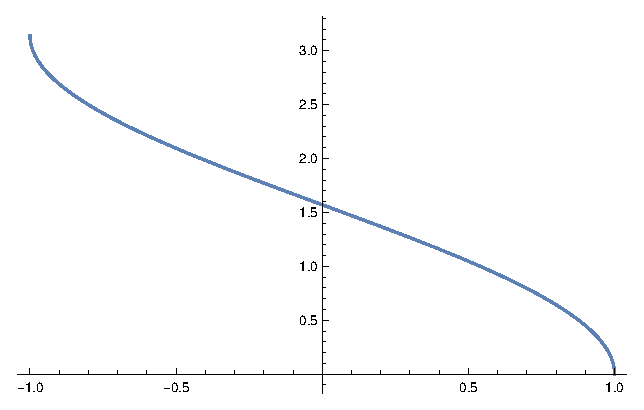
\includegraphics{chapters/appendices/KP_Mathematica/Kronig_Penney_model_transfer_matrix_gr1.eps}

\begin{doublespace}
\noindent\(\pmb{\text{kk}[\text{q$\_$},\text{epsilon$\_$}]\text{:=}\text{ArcCos}[\text{qq}[q,\text{epsilon}]]\text{                             }\text{(*
0 $<$ k $<$ Pi *)} }\)
\end{doublespace}

\begin{doublespace}
\noindent\(\pmb{\text{}}\\
\pmb{}\)
\end{doublespace}

\begin{doublespace}
\noindent\(\pmb{\text{(*} \text{Illustration}: \text{plot} \text{band} \text{structure} q(k) = \text{omega}(k)/v \text{for} -\text{Pi}<k<\text{Pi}
\text{in} \text{reduced} \text{zone} \text{scheme} \text{*)}}\\
\pmb{\text{(*} \text{for} \text{epsilon} = 1 \text{*)}}\)
\end{doublespace}

\begin{doublespace}
\noindent\(\pmb{\text{Plot}[\text{kk}[q,1],\{q,0,14\}]\text{         }\text{(*} \text{function} k(q), \text{range} 0 < k < \text{Pi}, \text{epsilon}
= 1 \text{*)} }\)
\end{doublespace}

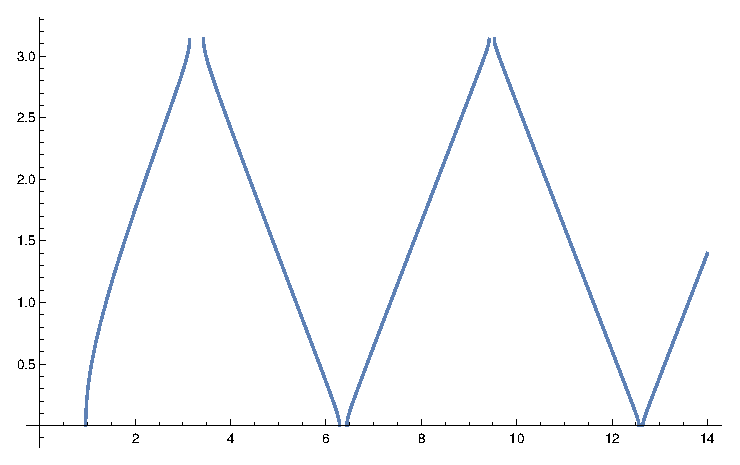
\includegraphics{chapters/appendices/KP_Mathematica/Kronig_Penney_model_transfer_matrix_gr2.eps}

\begin{doublespace}
\noindent\(\pmb{\text{kq}[\text{q$\_$},\text{epsilon$\_$}]\text{:=}\text{If}[\text{Abs}[\text{qq}[q,\text{epsilon}]]<1,\text{kk}[q,\text{epsilon}],100]\text{
    }\text{(*} k(q), \text{allow} \text{only} |q|<1 \text{*)}}\)
\end{doublespace}

\begin{doublespace}
\noindent\(\pmb{\text{(*} \text{use} \text{parametric} \text{plot} \text{to} \text{plot} \text{inverse} \text{function} q(k) \text{*)}}\)
\end{doublespace}

\begin{doublespace}
\noindent\(\pmb{\text{pos}=\text{ParametricPlot}[\{\text{kq}[q,1],q\},\{q,0,14\},\text{PlotRange}\to \{\{-\text{Pi}-0.1,\text{Pi}+0.1\},\{0,14\}\},}\\
\pmb{\text{PlotStyle}\to \{\{\text{Black},\text{Thickness}[0.007]\}\}, \text{AxesStyle}\to \text{Directive}[20],\text{Ticks}\to \{\{-\text{Pi},0,\text{Pi}\},\{2,4,8,10\}\}]}\)
\end{doublespace}

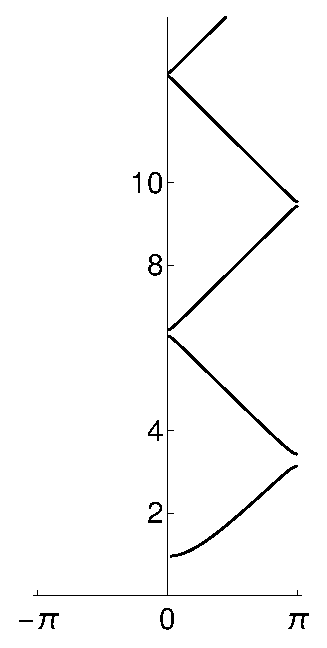
\includegraphics{chapters/appendices/KP_Mathematica/Kronig_Penney_model_transfer_matrix_gr3.eps}
\begin{doublespace}
\noindent\(\pmb{\text{neg}=\text{ParametricPlot}[\{-\text{kq}[q,1],q\},\{q,0,14\},\text{PlotRange}\to \{\{-\text{Pi}-0.1,\text{Pi}+0.1\},\{0,14\}\},}\\
\pmb{\text{PlotStyle}\to \{\{\text{Black},\text{Thickness}[0.007]\}\}, \text{AxesStyle}\to \text{Directive}[20],\text{Ticks}\to \{\{-\text{Pi},0,\text{Pi}\},\{2,4,8,10\}\}]}\)
\end{doublespace}

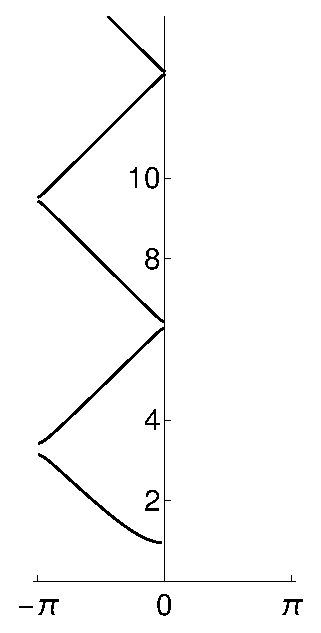
\includegraphics{chapters/appendices/KP_Mathematica/Kronig_Penney_model_transfer_matrix_gr4.eps}

\begin{doublespace}
\noindent\(\pmb{\text{pipos}=\text{ParametricPlot}[\{\text{Pi},q\},\{q,0,14\},\text{PlotRange}\to \{\{-\text{Pi}-0.1,\text{Pi}+0.1\},\{0,14\}\},\text{PlotStyle}\to
\{\{\text{Black},\text{Thickness}[0.0015]\}\}, }\\
\pmb{\text{AxesStyle}\to \text{Directive}[20],\text{Ticks}\to \{\{-\text{Pi},0,\text{Pi}\},\{2,4,8,10\}\}]}\)
\end{doublespace}

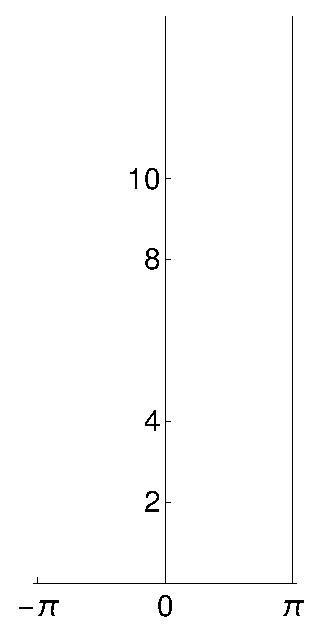
\includegraphics{chapters/appendices/KP_Mathematica/Kronig_Penney_model_transfer_matrix_gr5.eps}

\begin{doublespace}
\noindent\(\pmb{\text{pineg}=\text{ParametricPlot}[\{-\text{Pi},q\},\{q,0,14\},\text{PlotRange}\to \{\{-\text{Pi}-0.1,\text{Pi}+0.1\},\{0,14\}\},\text{PlotStyle}\to
\{\{\text{Black},\text{Thickness}[0.0015]\}\}, }\\
\pmb{\text{AxesStyle}\to \text{Directive}[20],\text{Ticks}\to \{\{-\text{Pi},0,\text{Pi}\},\{2,4,8,10\}\}]}\)
\end{doublespace}

\includegraphics{chapters/appendices/KP_Mathematica/Kronig_Penney_model_transfer_matrix_gr6.eps}

\begin{doublespace}
\noindent\(\pmb{\text{band}=\text{Show}[\text{neg},\text{pos},\text{pipos},\text{pineg}]}\)
\end{doublespace}

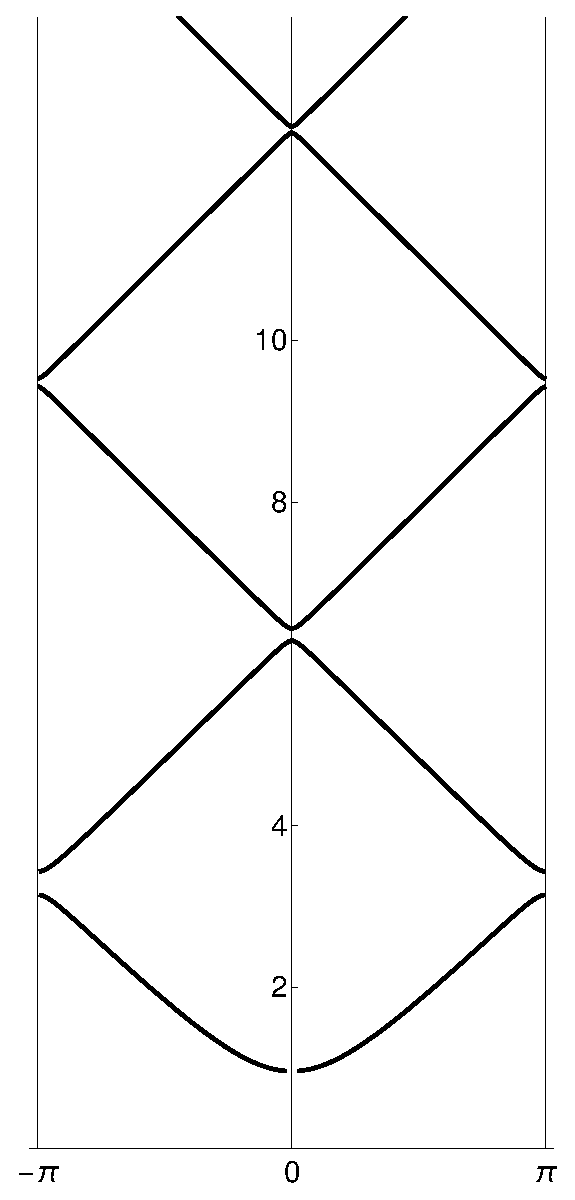
\includegraphics{chapters/appendices/KP_Mathematica/Kronig_Penney_model_transfer_matrix_gr7.eps}

\begin{doublespace}
\noindent\(\pmb{\text{Export}[\text{{``}bs.png{''}},\text{band},\text{ImageResolution}\to 300]}\)
\end{doublespace}

\begin{doublespace}
\noindent\(\text{bs.png}\)
\end{doublespace}

\begin{doublespace}
\noindent\(\pmb{\text{(* End Illustration *)}}\)
\end{doublespace}

\begin{doublespace}
\noindent\(\pmb{\text{}}\)
\end{doublespace}

\begin{doublespace}
\noindent\(\pmb{\text{(*} \text{Bloch} \text{functions} \text{Phi}(x) \text{with} \text{additional} \text{normalization} \text{*)} }\)
\end{doublespace}

\begin{doublespace}
\noindent\(\pmb{\text{(*} \text{allow} \text{only} |q|<1 \text{*)}}\)
\end{doublespace}

\begin{doublespace}
\noindent\(\pmb{\text{(*} \text{in} \text{what} \text{follows}: \text{index} 1 = +k, \text{index} 2 = -k \text{*)}}\)
\end{doublespace}

\begin{doublespace}
\noindent\(\pmb{\text{exp1}[\text{q$\_$},\text{epsilon$\_$},\text{n$\_$}]\text{:=}\text{If}[\text{Abs}[\text{qq}[q,\text{epsilon}]]<1,\text{Exp}[I
\text{kk}[q,\text{epsilon}] n],0]\text{      }\text{(* k1 $>$ 0 *)}}\)
\end{doublespace}

\begin{doublespace}
\noindent\(\pmb{\text{exp2}[\text{q$\_$},\text{epsilon$\_$},\text{n$\_$}]\text{:=}\text{If}[\text{Abs}[\text{qq}[q,\text{epsilon}]]<1,\text{Exp}[-I
\text{kk}[q,\text{epsilon}] n],0]\text{   }\text{(*} \text{k2} = -\text{k1} < 0 \text{*)}}\)
\end{doublespace}

\begin{doublespace}
\noindent\(\pmb{\text{(*} \text{phi1raw}, \text{phi2raw} \text{not} \text{correctly} \text{normalized}, \text{missing} \text{normalization} \text{factors}
\text{norm1}, \text{norm2} \text{below} \text{*)}}\)
\end{doublespace}

\begin{doublespace}
\noindent\(\pmb{\text{phi1raw}[\text{x$\_$},\text{n$\_$},\text{q$\_$},\text{epsilon$\_$}]\text{:=}}\\
\pmb{\text{exp1}[q,\text{epsilon},n] (\text{v1norm}[q,\text{epsilon}][[1]]\text{Exp}[I q (x-n)]+\text{v1norm}[q,\text{epsilon}][[2]]\text{Exp}[-I
q (x-n)])/}\\
\pmb{(\text{v1norm}[q,\text{epsilon}][[1]]+\text{v1norm}[q,\text{epsilon}][[2]])}\)
\end{doublespace}

\begin{doublespace}
\noindent\(\pmb{\text{phi2raw}[\text{x$\_$},\text{n$\_$},\text{q$\_$},\text{epsilon$\_$}]\text{:=}}\\
\pmb{\text{exp2}[q,\text{epsilon},n] (\text{v2norm}[q,\text{epsilon}][[1]]\text{Exp}[I q (x-n)]+\text{v2norm}[q,\text{epsilon}][[2]]\text{Exp}[-I
q (x-n)])/}\\
\pmb{(\text{v2norm}[q,\text{epsilon}][[1]]+\text{v2norm}[q,\text{epsilon}][[2]])}\)
\end{doublespace}

\begin{doublespace}
\noindent\(\pmb{\text{}}\)
\end{doublespace}

\begin{doublespace}
\noindent\(\pmb{\text{}}\)
\end{doublespace}

\begin{doublespace}
\noindent\(\pmb{\text{(*} \text{functions} u(x) \text{for} 0<x<1, \text{then} \text{periodically} \text{extended} \text{*)}}\)
\end{doublespace}

\begin{doublespace}
\noindent\(\pmb{\text{u1raw}[\text{x$\_$},\text{q$\_$},\text{epsilon$\_$}]\text{:=}}\\
\pmb{(\text{v1norm}[q,\text{epsilon}][[1]]\text{Exp}[I (q-\text{kk}[q,\text{epsilon}])(x-1)]+\text{v1norm}[q,\text{epsilon}][[2]]\text{Exp}[-I (q+\text{kk}[q,\text{epsilon}])(x-1)])/}\\
\pmb{(\text{v1norm}[q,\text{epsilon}][[1]]+\text{v1norm}[q,\text{epsilon}][[2]])}\)
\end{doublespace}

\begin{doublespace}
\noindent\(\pmb{\text{norm1}[\text{q$\_$},\text{epsilon$\_$}] \text{:=}\text{Sqrt}[\text{NIntegrate}[\text{u1raw}[x,q,\text{epsilon}]\text{Conjugate}[\text{u1raw}[x,q,\text{epsilon}]],\{x,0,1\}]]}\)
\end{doublespace}

\begin{doublespace}
\noindent\(\pmb{\text{u1}[\text{x$\_$},\text{q$\_$},\text{epsilon$\_$}] \text{:=}\text{u1raw}[x,q,\text{epsilon}]/\text{norm1}[q,\text{epsilon}]\text{
     }}\)
\end{doublespace}

\begin{doublespace}
\noindent\(\pmb{\text{NIntegrate}[\text{u1}[x,0.3,0.7]\text{Conjugate}[\text{u1}[x,0.3,0.7]],\{x,0,1\}]\text{      }\text{(* u1 correctly normalized
*)} }\)
\end{doublespace}

\begin{doublespace}
\noindent\(1.\)
\end{doublespace}

\begin{doublespace}
\noindent\(\pmb{\text{u2raw}[\text{x$\_$},\text{q$\_$},\text{epsilon$\_$}]\text{:=}}\\
\pmb{(\text{v2norm}[q,\text{epsilon}][[1]]\text{Exp}[I (q+\text{kk}[q,\text{epsilon}])(x-1)]+\text{v2norm}[q,\text{epsilon}][[2]]\text{Exp}[-I (q-\text{kk}[q,\text{epsilon}])(x-1)])/}\\
\pmb{(\text{v2norm}[q,\text{epsilon}][[1]]+\text{v2norm}[q,\text{epsilon}][[2]])}\)
\end{doublespace}

\begin{doublespace}
\noindent\(\pmb{\text{norm2}[\text{q$\_$},\text{epsilon$\_$}] \text{:=}\text{Sqrt}[\text{NIntegrate}[\text{u2raw}[x,q,\text{epsilon}]\text{Conjugate}[\text{u2raw}[x,q,\text{epsilon}]],\{x,0,1\}]]}\)
\end{doublespace}

\begin{doublespace}
\noindent\(\pmb{\text{u2}[\text{x$\_$},\text{q$\_$},\text{epsilon$\_$}] \text{:=}\text{u2raw}[x,q,\text{epsilon}]/\text{norm2}[q,\text{epsilon}]}\)
\end{doublespace}

\begin{doublespace}
\noindent\(\pmb{\text{NIntegrate}[\text{u2}[x,0.3,0.7]\text{Conjugate}[\text{u2}[x,0.3,0.7]],\{x,0,1\}]\text{      }\text{(* u2 correctly normalized
*)} }\)
\end{doublespace}

\begin{doublespace}
\noindent\(1.\)
\end{doublespace}

\begin{doublespace}
\noindent\(\pmb{\text{}}\)
\end{doublespace}

\begin{doublespace}
\noindent\(\pmb{\text{(*} \text{functions} c(q), d(q) \text{*)} }\)
\end{doublespace}

\begin{doublespace}
\noindent\(\pmb{\text{u1prime}[\text{x$\_$},\text{q$\_$},\text{epsilon$\_$}]\text{:=}\text{Derivative}[1,0,0][\text{u1raw}][x,q,\text{epsilon}]/\text{norm1}[q,\text{epsilon}]}\)
\end{doublespace}

\begin{doublespace}
\noindent\(\pmb{\text{u2prime}[\text{x$\_$},\text{q$\_$},\text{epsilon$\_$}]\text{:=}\text{Derivative}[1,0,0][\text{u2raw}][x,q,\text{epsilon}]/\text{norm2}[q,\text{epsilon}]}\)
\end{doublespace}

\begin{doublespace}
\noindent\(\pmb{c[\text{q$\_$},\text{epsilon$\_$}]\text{:=}\text{u1}[0,q,\text{epsilon}]\text{    }\text{(* cal C in thesis *)}}\)
\end{doublespace}

\begin{doublespace}
\noindent\(\pmb{\text{(*} c \text{real} \text{and} \text{equal} \text{for} (1), (2) \text{*)}}\)
\end{doublespace}

\begin{doublespace}
\noindent\(\pmb{c[0.9,0.2]}\)
\end{doublespace}

\begin{doublespace}
\noindent\(0.982811\, -\text{5.4556988634997206$\grave{ }$*${}^{\wedge}$-17} i\)
\end{doublespace}

\begin{doublespace}
\noindent\(\pmb{\text{u2}[0,0.9,0.2]}\)
\end{doublespace}

\begin{doublespace}
\noindent\(0.982811\, -\text{1.8549376135899046$\grave{ }$*${}^{\wedge}$-15} i\)
\end{doublespace}

\begin{doublespace}
\noindent\(\pmb{c[2,3]}\)
\end{doublespace}

\begin{doublespace}
\noindent\(0.762883\, +\text{3.469446951953614$\grave{ }$*${}^{\wedge}$-17} i\)
\end{doublespace}

\begin{doublespace}
\noindent\(\pmb{\text{u2}[0,2,3]}\)
\end{doublespace}

\begin{doublespace}
\noindent\(0.762883\, -\text{4.163336342344337$\grave{ }$*${}^{\wedge}$-17} i\)
\end{doublespace}

\begin{doublespace}
\noindent\(\pmb{d[\text{q$\_$},\text{epsilon$\_$}]\text{:=}\text{u1prime}[0,q,\text{epsilon}]\text{      }\text{(* cal D in thesis *)}}\)
\end{doublespace}

\begin{doublespace}
\noindent\(\pmb{\text{(*} d \text{complex} \text{and} \text{conjugate} \text{for} (1), (2) \text{*)}}\)
\end{doublespace}

\begin{doublespace}
\noindent\(\pmb{d[0.9,0.2]}\)
\end{doublespace}

\begin{doublespace}
\noindent\(0.0982811\, +0.0269644 i\)
\end{doublespace}

\begin{doublespace}
\noindent\(\pmb{\text{u2prime}[0,0.9,0.2]}\)
\end{doublespace}

\begin{doublespace}
\noindent\(0.0982811\, -0.0269644 i\)
\end{doublespace}

\begin{doublespace}
\noindent\(\pmb{d[2,3]}\)
\end{doublespace}

\begin{doublespace}
\noindent\(1.14432\, +0.624518 i\)
\end{doublespace}

\begin{doublespace}
\noindent\(\pmb{\text{u2prime}[0,2,3]}\)
\end{doublespace}

\begin{doublespace}
\noindent\(1.14432\, -0.624518 i\)
\end{doublespace}

\begin{doublespace}
\noindent\(\pmb{\text{(*} \text{Note}: \text{For} \text{our} \text{calculation} \text{we} \text{need} C \text{and} D \text{as} \text{functions} \text{of}
k \text{instead} \text{*)}}\\
\pmb{\text{(*} \text{of} q=\text{omega}. \text{For} \text{this} \text{we} \text{need} \text{the} \text{function} q(k) \text{which} \text{is} \text{the}
\text{inverse}\text{  }\text{*)}}\\
\pmb{\text{(*} \text{of} \text{the} \text{function} k(q). \text{See} \text{illustration} \text{at} \text{the} \text{beginnng} \text{of} \text{the}
\text{notebook}. \text{*)}}\\
\pmb{\text{(*} \text{If} \text{we} \text{have} q(k) \text{then} c[k, \text{epsilon}] = \text{u1}[0, q(k), \text{epsilon}] \text{and} \text{*)} }\\
\pmb{\text{(*} d[k, \text{epsilon}] = \text{uprime1}[0, q(k), \text{epsilon}] \text{*)}}\)
\end{doublespace}

\begin{doublespace}
\noindent\(\pmb{\text{}}\)
\end{doublespace}

\begin{doublespace}
\noindent\(\pmb{\text{(* Illustrations and side calculations *)}}\)
\end{doublespace}

\begin{doublespace}
\noindent\(\pmb{\text{}}\)
\end{doublespace}

\begin{doublespace}
\noindent\(\pmb{\text{(*} \text{Properties} \text{of} \text{u1}, \text{u2} \text{and} \text{derivatives} \text{*)}}\)
\end{doublespace}

\begin{doublespace}
\noindent\(\pmb{\text{(*} \text{Show} \text{u1}(0)=\text{u1}(1)=\text{u2}(0)=\text{u2}(1) \text{and} \text{real} \text{*)}}\)
\end{doublespace}

\begin{doublespace}
\noindent\(\pmb{\text{Abs}[\text{qq}[0.7,0.3]]\text{    }\text{(*} \text{needs} \text{to} \text{be} <1 \text{*)}}\)
\end{doublespace}

\begin{doublespace}
\noindent\(0.902889\)
\end{doublespace}

\begin{doublespace}
\noindent\(\pmb{\text{u1}[0,0.7,0.3] \text{//}N}\)
\end{doublespace}

\begin{doublespace}
\noindent\(0.975105\, -\text{1.6238756426406062$\grave{ }$*${}^{\wedge}$-16} i\)
\end{doublespace}

\begin{doublespace}
\noindent\(\pmb{\text{u1}[1,0.7,0.3] \text{//}N}\)
\end{doublespace}

\begin{doublespace}
\noindent\(0.975105\, +0. i\)
\end{doublespace}

\begin{doublespace}
\noindent\(\pmb{\text{u2}[0,0.7,0.3] \text{//}N}\)
\end{doublespace}

\begin{doublespace}
\noindent\(0.975105\, -\text{2.1651675235208085$\grave{ }$*${}^{\wedge}$-16} i\)
\end{doublespace}

\begin{doublespace}
\noindent\(\pmb{\text{u2}[1,0.7,0.3] \text{//}N}\)
\end{doublespace}

\begin{doublespace}
\noindent\(0.975105\, +\text{5.412918808802021$\grave{ }$*${}^{\wedge}$-17} i\)
\end{doublespace}

\begin{doublespace}
\noindent\(\pmb{\text{Abs}[\text{qq}[0.9,0.2]]\text{    }\text{(*} \text{needs} \text{to} \text{be} <1 \text{*)}}\)
\end{doublespace}

\begin{doublespace}
\noindent\(0.708646\)
\end{doublespace}

\begin{doublespace}
\noindent\(\pmb{\text{u1}[0,0.9,0.2] \text{//}N}\)
\end{doublespace}

\begin{doublespace}
\noindent\(0.982811\, -\text{5.4556988634997206$\grave{ }$*${}^{\wedge}$-17} i\)
\end{doublespace}

\begin{doublespace}
\noindent\(\pmb{\text{u1}[1,0.9,0.2] \text{//}N}\)
\end{doublespace}

\begin{doublespace}
\noindent\(0.982811\, +0. i\)
\end{doublespace}

\begin{doublespace}
\noindent\(\pmb{\text{u2}[0,0.9,0.2] \text{//}N}\)
\end{doublespace}

\begin{doublespace}
\noindent\(0.982811\, -\text{1.8549376135899046$\grave{ }$*${}^{\wedge}$-15} i\)
\end{doublespace}

\begin{doublespace}
\noindent\(\pmb{\text{u2}[1,0.9,0.2] \text{//}N}\)
\end{doublespace}

\begin{doublespace}
\noindent\(0.982811\, +0. i\)
\end{doublespace}

\begin{doublespace}
\noindent\(\pmb{\text{Abs}[\text{qq}[0.3,0]]\text{    }\text{(*} \text{needs} \text{to} \text{be} <1 \text{*)}}\)
\end{doublespace}

\begin{doublespace}
\noindent\(0.955336\)
\end{doublespace}

\begin{doublespace}
\noindent\(\pmb{\text{(*} \text{Show} \text{u1}=\text{u2}=1 \text{for} \text{epsilon}=0 \text{*)}}\)
\end{doublespace}

\begin{doublespace}
\noindent\(\pmb{\text{u1}[0.9,0.3,0.0000000001]}\)
\end{doublespace}

\begin{doublespace}
\noindent\(1.\, -\text{3.627653732932283$\grave{ }$*${}^{\wedge}$-13} i\)
\end{doublespace}

\begin{doublespace}
\noindent\(\pmb{\text{u2}[0.9,0.3,0.0000000001]}\)
\end{doublespace}

\begin{doublespace}
\noindent\(1.\, +\text{4.137104930015478$\grave{ }$*${}^{\wedge}$-8} i\)
\end{doublespace}

\begin{doublespace}
\noindent\(\pmb{\text{}}\)
\end{doublespace}

\begin{doublespace}
\noindent\(\pmb{\text{(*} \text{Show}: \text{u2} = \text{Conjugate}[\text{u1}] \text{if} \text{Abs}[\text{qq}]<1 \text{*)}}\)
\end{doublespace}

\begin{doublespace}
\noindent\(\pmb{\text{Abs}[\text{qq}[0.9,0.2]]\text{    }\text{(*} \text{needs} \text{to} \text{be} <1 \text{*)}}\)
\end{doublespace}

\begin{doublespace}
\noindent\(0.708646\)
\end{doublespace}

\begin{doublespace}
\noindent\(\pmb{\text{u1}[0.3,0.9,0.2]}\)
\end{doublespace}

\begin{doublespace}
\noindent\(1.00448\, +0.00233511 i\)
\end{doublespace}

\begin{doublespace}
\noindent\(\pmb{\text{u2}[0.3,0.9,0.2]}\)
\end{doublespace}

\begin{doublespace}
\noindent\(1.00448\, -0.00233511 i\)
\end{doublespace}

\begin{doublespace}
\noindent\(\pmb{\text{(*} \text{plot} \text{real} \text{part} \text{of} u(x) \text{for} \text{epsilon} = 0.2 \text{*)}}\)
\end{doublespace}

\begin{doublespace}
\noindent\(\pmb{\text{pu1}=\text{Plot}[\text{Re}[\text{u1}[x,0.9,0.2]],\{x,0,1\},\text{PlotStyle}\to \text{Black}]}\)
\end{doublespace}

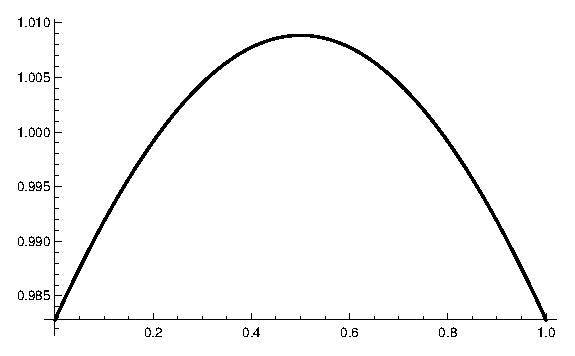
\includegraphics{chapters/appendices/KP_Mathematica/Kronig_Penney_model_transfer_matrix_gr8.eps}

\begin{doublespace}
\noindent\(\pmb{\text{pu2}=\text{Plot}[\text{Re}[\text{u2}[x,0.9,0.2]],\{x,0,1\},\text{PlotStyle}\to \{\text{Red},\text{Dashed}\}]}\)
\end{doublespace}

\includegraphics{chapters/appendices/KP_Mathematica/Kronig_Penney_model_transfer_matrix_gr9.eps}

\begin{doublespace}
\noindent\(\pmb{\text{Show}[\text{pu1},\text{pu2}]}\)
\end{doublespace}

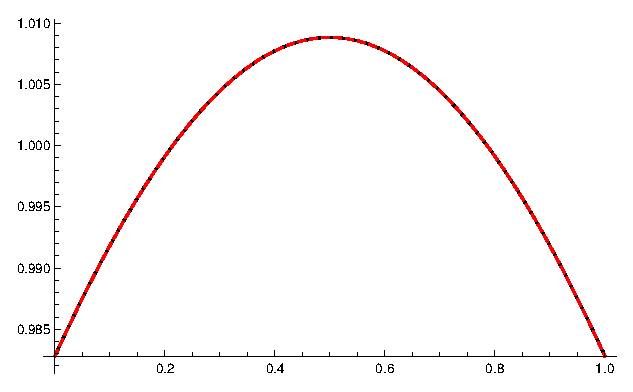
\includegraphics{chapters/appendices/KP_Mathematica/Kronig_Penney_model_transfer_matrix_gr10.eps}

\begin{doublespace}
\noindent\(\pmb{\text{(*} \text{plot} \text{imaginary} \text{part} \text{of} u(x) \text{*)}}\)
\end{doublespace}

\begin{doublespace}
\noindent\(\pmb{\text{pu3}=\text{Plot}[\text{Im}[\text{u1}[x,0.9,0.2]],\{x,0,1\},\text{PlotStyle}\to \text{Black}]}\)
\end{doublespace}

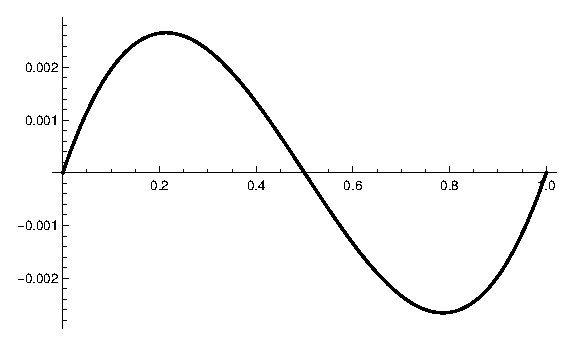
\includegraphics{chapters/appendices/KP_Mathematica/Kronig_Penney_model_transfer_matrix_gr11.eps}

\begin{doublespace}
\noindent\(\pmb{\text{pu4}=\text{Plot}[\text{Im}[\text{u2}[x,0.9,0.2]],\{x,0,1\},\text{PlotStyle}\to \{\text{Red},\text{Dashed}\}]}\)
\end{doublespace}

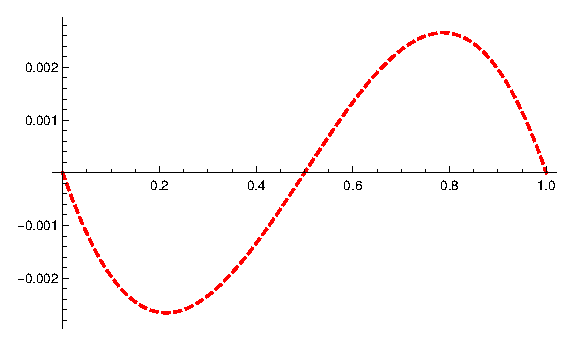
\includegraphics{chapters/appendices/KP_Mathematica/Kronig_Penney_model_transfer_matrix_gr12.eps}

\begin{doublespace}
\noindent\(\pmb{\text{Show}[\text{pu3},\text{pu4}]}\)
\end{doublespace}

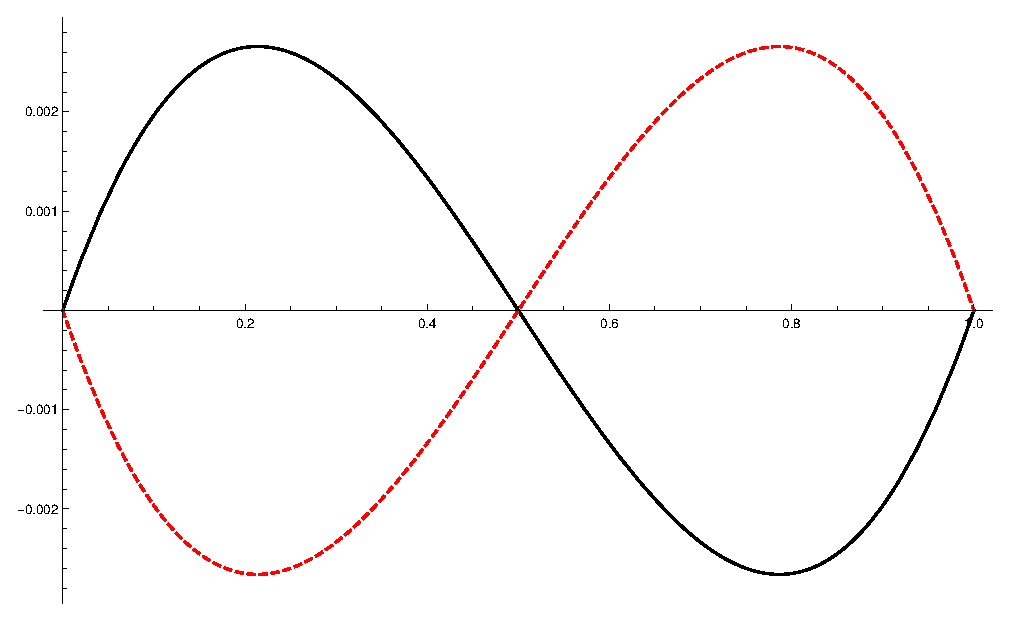
\includegraphics{chapters/appendices/KP_Mathematica/Kronig_Penney_model_transfer_matrix_gr13.eps}

\begin{doublespace}
\noindent\(\pmb{\text{}}\)
\end{doublespace}

\begin{doublespace}
\noindent\(\pmb{\text{(*} \text{Illustration}: \text{plot} u(x) \text{for} \text{epsilon} = 1 \text{and} q=2 \text{*)}}\)
\end{doublespace}

\begin{doublespace}
\noindent\(\pmb{\text{Abs}[\text{qq}[2,1]]\text{  }\text{//}N\text{   }\text{(*} \text{needs} \text{to} \text{be} <1 \text{*)}}\)
\end{doublespace}

\begin{doublespace}
\noindent\(0.188822\)
\end{doublespace}

\begin{doublespace}
\noindent\(\pmb{\text{u1}[0.4,2,1]}\)
\end{doublespace}

\begin{doublespace}
\noindent\(1.05025\, +0.0207882 i\)
\end{doublespace}

\begin{doublespace}
\noindent\(\pmb{\text{u2}[0.4,2,1]}\)
\end{doublespace}

\begin{doublespace}
\noindent\(1.05025\, -0.0207882 i\)
\end{doublespace}

\begin{doublespace}
\noindent\(\pmb{\text{(*} \text{plot} \text{real} \text{part} \text{of} u(x) \text{*)}}\)
\end{doublespace}

\begin{doublespace}
\noindent\(\pmb{\text{pu5}=\text{Plot}[\text{Re}[\text{u1}[x,2,1]],\{x,0,1\},\text{PlotStyle}\to \text{Black}]}\)
\end{doublespace}

\includegraphics{chapters/appendices/KP_Mathematica/Kronig_Penney_model_transfer_matrix_gr14.eps}

\begin{doublespace}
\noindent\(\pmb{\text{pu6}=\text{Plot}[\text{Re}[\text{u2}[x,2,1]],\{x,0,1\},\text{PlotStyle}\to \{\text{Red},\text{Dashed}\}]}\)
\end{doublespace}

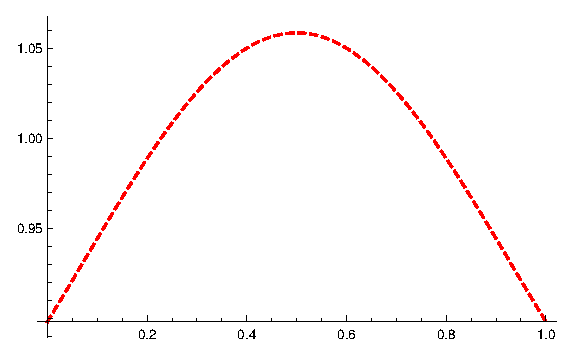
\includegraphics{chapters/appendices/KP_Mathematica/Kronig_Penney_model_transfer_matrix_gr15.eps}

\begin{doublespace}
\noindent\(\pmb{\text{Show}[\text{pu5},\text{pu6}]}\)
\end{doublespace}

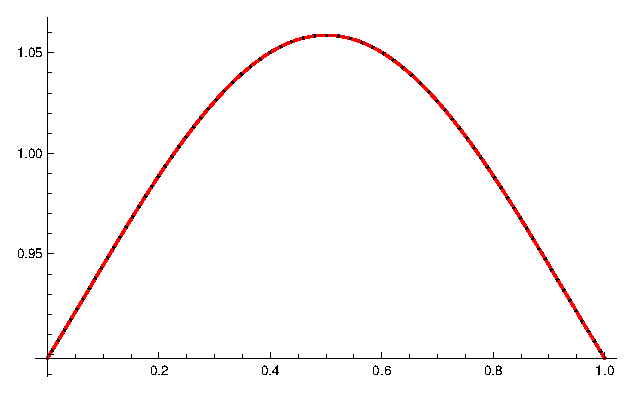
\includegraphics{chapters/appendices/KP_Mathematica/Kronig_Penney_model_transfer_matrix_gr16.eps}

\begin{doublespace}
\noindent\(\pmb{\text{(*} \text{plot} \text{imaginary} \text{part} \text{of} u(x) \text{*)}}\)
\end{doublespace}

\begin{doublespace}
\noindent\(\pmb{\text{pu7}=\text{Plot}[\text{Im}[\text{u1}[x,2,1]],\{x,0,1\},\text{PlotStyle}\to \text{Black}]}\)
\end{doublespace}

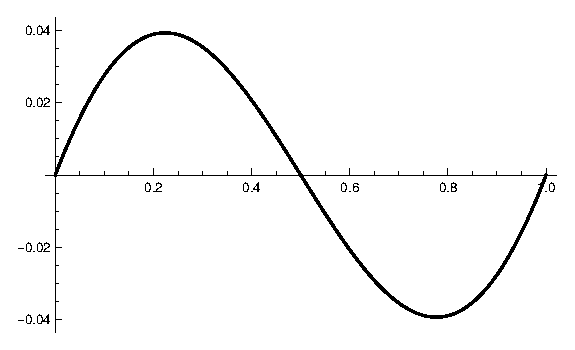
\includegraphics{chapters/appendices/KP_Mathematica/Kronig_Penney_model_transfer_matrix_gr17.eps}

\begin{doublespace}
\noindent\(\pmb{\text{pu8}=\text{Plot}[\text{Im}[\text{u2}[x,2,1]],\{x,0,1\},\text{PlotStyle}\to \{\text{Red},\text{Dashed}\}]}\)
\end{doublespace}

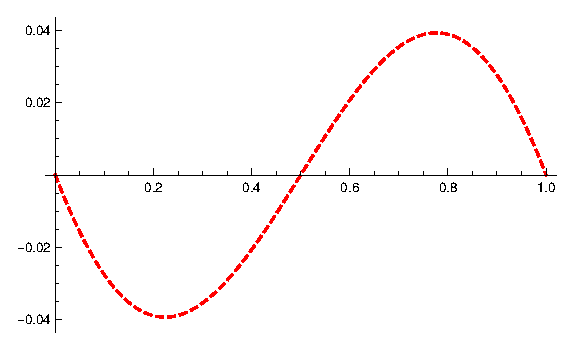
\includegraphics{chapters/appendices/KP_Mathematica/Kronig_Penney_model_transfer_matrix_gr18.eps}

\begin{doublespace}
\noindent\(\pmb{\text{Show}[\text{pu7},\text{pu8}]}\)
\end{doublespace}

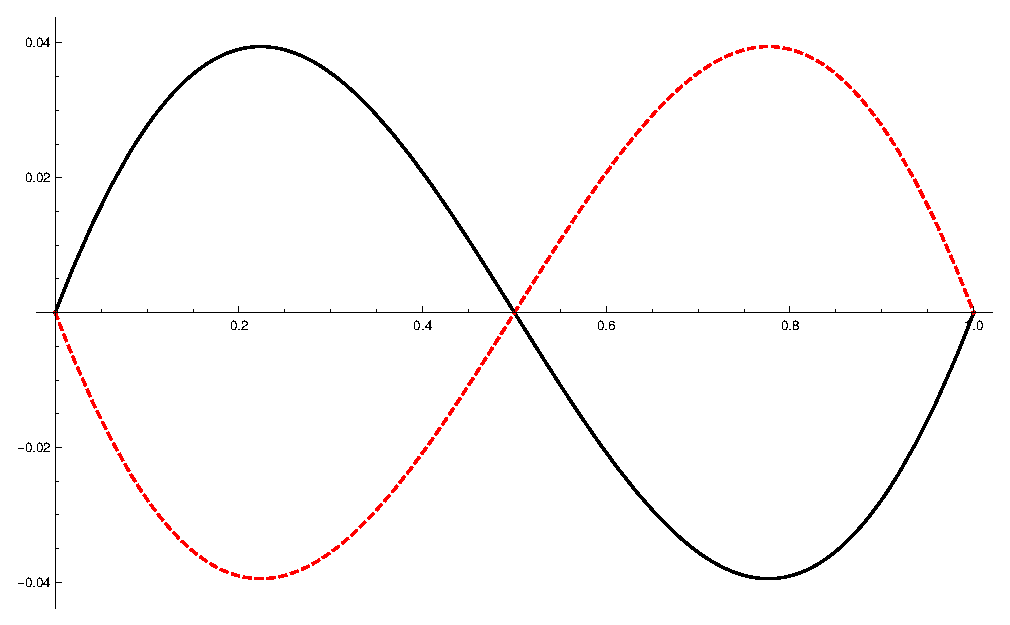
\includegraphics{chapters/appendices/KP_Mathematica/Kronig_Penney_model_transfer_matrix_gr19.eps}

\begin{doublespace}
\noindent\(\pmb{\text{}}\)
\end{doublespace}

\begin{doublespace}
\noindent\(\pmb{\text{Abs}[\text{qq}[1.1,1.348]]\text{    }\text{(*} \text{epsilon}=1.348 \text{is} \text{critical} \text{value} \text{for} q=1.1
\text{*)}}\)
\end{doublespace}

\begin{doublespace}
\noindent\(0.999663\)
\end{doublespace}

\begin{doublespace}
\noindent\(\pmb{\text{Plot}[\{\text{Re}[\text{u1}[0.4,1.1,\text{eps}]],\text{Re}[\text{u2}[0.4,1.1,\text{eps}]]\},\{\text{eps},0,2\},\text{PlotStyle}\to
\text{Black}]}\)
\end{doublespace}

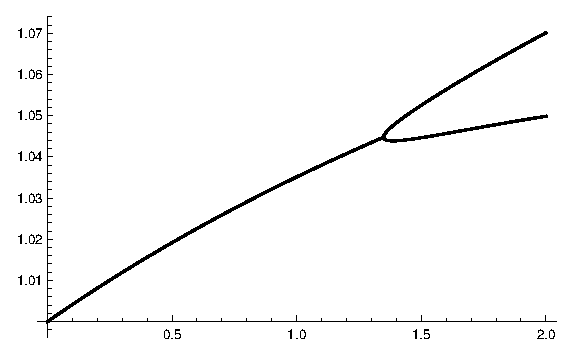
\includegraphics{chapters/appendices/KP_Mathematica/Kronig_Penney_model_transfer_matrix_gr20.eps}

\begin{doublespace}
\noindent\(\pmb{\text{Plot}[\{\text{Im}[\text{u1}[0.4,1.1,\text{eps}]],\text{Im}[\text{u2}[0.4,1.1,\text{eps}]]\},\{\text{eps},0,2\},\text{PlotStyle}\to
\text{Black}]}\)
\end{doublespace}

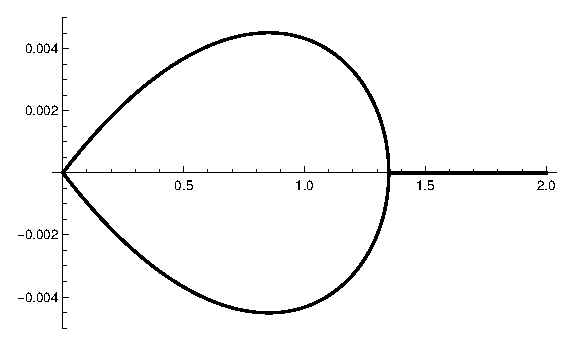
\includegraphics{chapters/appendices/KP_Mathematica/Kronig_Penney_model_transfer_matrix_gr21.eps}

\begin{doublespace}
\noindent\(\pmb{\text{}}\)
\end{doublespace}

\begin{doublespace}
\noindent\(\pmb{\text{(*} \text{Show}: \text{u2}'[0] = \text{Conjugate}[\text{u1}'[0]] \text{if} \text{Abs}[\text{qq}]<1 \text{*)}}\)
\end{doublespace}

\begin{doublespace}
\noindent\(\pmb{\text{Abs}[\text{qq}[0.9,0.2]]\text{    }\text{(*} \text{needs} \text{to} \text{be} <1 \text{*)}}\)
\end{doublespace}

\begin{doublespace}
\noindent\(0.708646\)
\end{doublespace}

\begin{doublespace}
\noindent\(\pmb{\text{u1prime}[0,0.9,0.2]}\)
\end{doublespace}

\begin{doublespace}
\noindent\(0.0982811\, +0.0269644 i\)
\end{doublespace}

\begin{doublespace}
\noindent\(\pmb{\text{u2prime}[0,0.9,0.2]}\)
\end{doublespace}

\begin{doublespace}
\noindent\(0.0982811\, -0.0269644 i\)
\end{doublespace}

\begin{doublespace}
\noindent\(\pmb{\text{Abs}[\text{qq}[2,3]] \text{//}N\text{   }\text{(*} \text{needs} \text{to} \text{be} <1 \text{*)}}\)
\end{doublespace}

\begin{doublespace}
\noindent\(0.265826\)
\end{doublespace}

\begin{doublespace}
\noindent\(\pmb{\text{u1prime}[0,2,3]}\)
\end{doublespace}

\begin{doublespace}
\noindent\(1.14432\, +0.624518 i\)
\end{doublespace}

\begin{doublespace}
\noindent\(\pmb{\text{u2prime}[0,2,3]}\)
\end{doublespace}

\begin{doublespace}
\noindent\(1.14432\, -0.624518 i\)
\end{doublespace}

\begin{doublespace}
\noindent\(\pmb{\text{(*} \text{END} \text{properties} \text{of} \text{u1}, \text{u2} \text{and} \text{derivatives} \text{*)}}\)
\end{doublespace}

\begin{doublespace}
\noindent\(\pmb{\text{}}\\
\pmb{}\)
\end{doublespace}

\begin{doublespace}
\noindent\(\pmb{\text{(*} \text{Plot} \text{real} \text{and} \text{imaginary} \text{parts} \text{of} \text{Bloch} \text{functions} \text{Phi$\_$raw}(x)
\text{*)}}\)
\end{doublespace}

\begin{doublespace}
\noindent\(\pmb{\text{(*} \text{Show} \text{Phi$\_$}2\text{$\_$raw} = \text{complex} \text{conjugate} \text{Phi$\_$}1\text{$\_$raw} \text{*)}}\)
\end{doublespace}

\begin{doublespace}
\noindent\(\pmb{\text{Abs}[\text{qq}[1,1]]\text{  }\text{//}N\text{  }\text{(*} \text{needs} \text{to} \text{be} <1 \text{*)}}\)
\end{doublespace}

\begin{doublespace}
\noindent\(0.961038\)
\end{doublespace}

\begin{doublespace}
\noindent\(\pmb{\text{p1}=\text{Plot}[\text{Re}[\text{phi1raw}[x,\text{Ceiling}[x],1,1]],\{x,0,20\},\text{PlotStyle}\to \text{Black}]}\)
\end{doublespace}

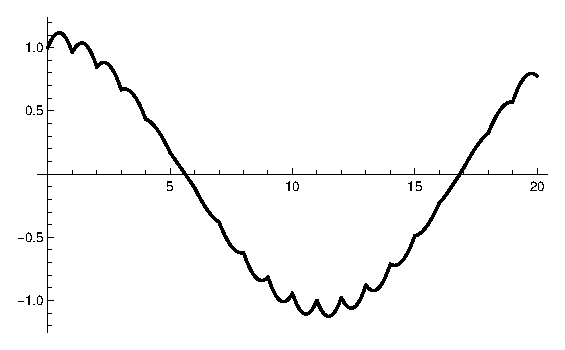
\includegraphics{chapters/appendices/KP_Mathematica/Kronig_Penney_model_transfer_matrix_gr22.eps}

\begin{doublespace}
\noindent\(\pmb{\text{p2}=\text{Plot}[\text{Re}[\text{phi2raw}[x,\text{Ceiling}[x],1,1]],\{x,0,20\},\text{PlotStyle}\to \{\text{Red},\text{Dashed}\}]\text{
 }\text{(*} \text{same} \text{as} \text{Re}(\text{phi1raw}) \text{*)}}\)
\end{doublespace}

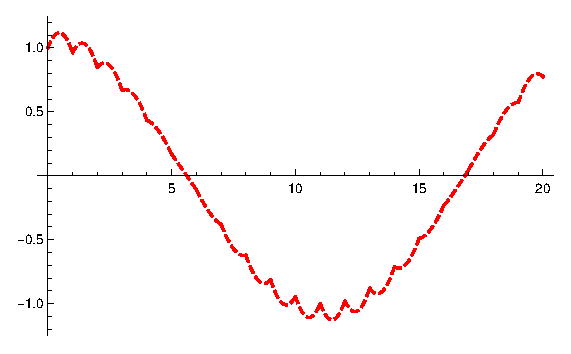
\includegraphics{chapters/appendices/KP_Mathematica/Kronig_Penney_model_transfer_matrix_gr23.eps}

\begin{doublespace}
\noindent\(\pmb{\text{Show}[\text{p1},\text{p2}]}\)
\end{doublespace}

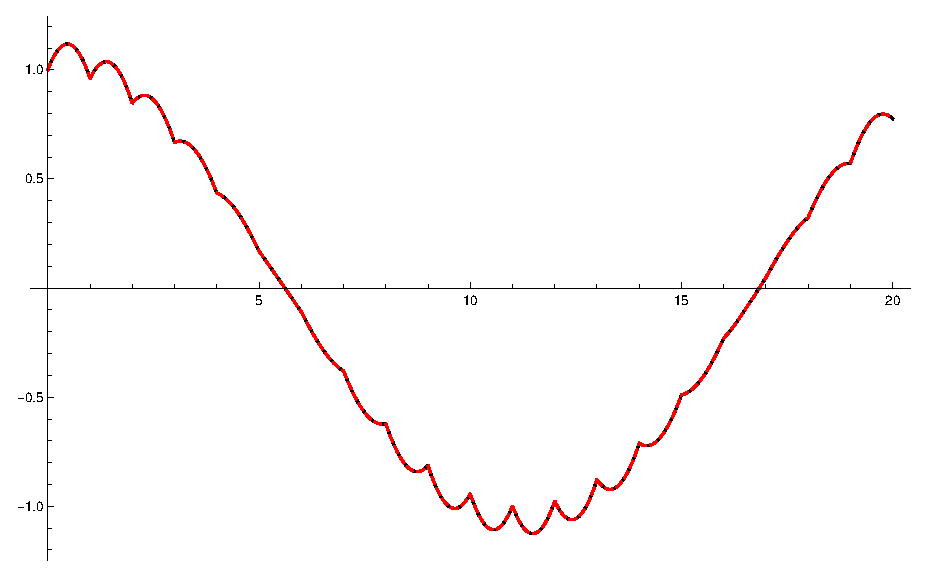
\includegraphics{chapters/appendices/KP_Mathematica/Kronig_Penney_model_transfer_matrix_gr24.eps}

\begin{doublespace}
\noindent\(\pmb{\text{p3}=\text{Plot}[\text{Im}[\text{phi1raw}[x,\text{Ceiling}[x],1,1]],\{x,0,20\},\text{PlotStyle}\to \text{Black}]}\)
\end{doublespace}

\includegraphics{chapters/appendices/KP_Mathematica/Kronig_Penney_model_transfer_matrix_gr25.eps}

\begin{doublespace}
\noindent\(\pmb{\text{p4}=\text{Plot}[\text{Im}[\text{phi2raw}[x,\text{Ceiling}[x],1,1]],\{x,0,20\},\text{PlotStyle}\to \{\text{Red},\text{Dashed}\}]\text{
 }\text{(*} -\text{Im}(\text{phi1raw}) \text{*)}}\)
\end{doublespace}

\includegraphics{chapters/appendices/KP_Mathematica/Kronig_Penney_model_transfer_matrix_gr26.eps}

\begin{doublespace}
\noindent\(\pmb{\text{Show}[\text{p3},\text{p4}]}\)
\end{doublespace}

\includegraphics{chapters/appendices/KP_Mathematica/Kronig_Penney_model_transfer_matrix_gr27.eps}

\begin{doublespace}
\noindent\(\pmb{\text{}}\\
\pmb{}\\
\pmb{}\\
\pmb{}\)
\end{doublespace}

\begin{doublespace}
\noindent\(\pmb{\text{(*} \text{Show} \text{that} \text{phi1raw}(x=n,n,q,\text{epsilon}) = \text{Exp}(i k n) \text{*)}}\)
\end{doublespace}

\begin{doublespace}
\noindent\(\pmb{\text{phi1raw}[7,7,0.9,0.2] \text{//}N}\)
\end{doublespace}

\begin{doublespace}
\noindent\(0.696237\, -0.717812 i\)
\end{doublespace}

\begin{doublespace}
\noindent\(\pmb{\text{Exp}[I \text{kk}[0.9,0.2] 7]\text{  }\text{//}N}\)
\end{doublespace}

\begin{doublespace}
\noindent\(0.696237\, -0.717812 i\)
\end{doublespace}

\begin{doublespace}
\noindent\(\pmb{\text{phi1raw}[8,8,2,3] \text{//}N}\)
\end{doublespace}

\begin{doublespace}
\noindent\(-0.549437-0.835535 i\)
\end{doublespace}

\begin{doublespace}
\noindent\(\pmb{\text{Exp}[I \text{kk}[2,3] 8]\text{  }\text{//}N}\)
\end{doublespace}

\begin{doublespace}
\noindent\(-0.549437-0.835535 i\)
\end{doublespace}

\begin{doublespace}
\noindent\(\pmb{\text{}}\)
\end{doublespace}

\begin{doublespace}
\noindent\(\pmb{\text{(*} \text{Show} \text{that} \text{phi2raw}(x=n,n,q,\text{epsilon}) = \text{Exp}(-i k n) \text{*)}}\)
\end{doublespace}

\begin{doublespace}
\noindent\(\pmb{\text{phi2raw}[7,7,0.9,0.2] \text{//}N}\)
\end{doublespace}

\begin{doublespace}
\noindent\(0.696237\, +0.717812 i\)
\end{doublespace}

\begin{doublespace}
\noindent\(\pmb{\text{Exp}[-I \text{kk}[0.9,0.2] 7]\text{  }\text{//}N}\)
\end{doublespace}

\begin{doublespace}
\noindent\(0.696237\, +0.717812 i\)
\end{doublespace}

\begin{doublespace}
\noindent\(\pmb{\text{phi2raw}[8,8,2,3] \text{//}N}\)
\end{doublespace}

\begin{doublespace}
\noindent\(-0.549437+0.835535 i\)
\end{doublespace}

\begin{doublespace}
\noindent\(\pmb{\text{Exp}[-I \text{kk}[2,3] 8]\text{  }\text{//}N}\)
\end{doublespace}

\begin{doublespace}
\noindent\(-0.549437+0.835535 i\)
\end{doublespace}

\begin{doublespace}
\noindent\(\pmb{\text{}}\)
\end{doublespace}

\begin{doublespace}
\noindent\(\pmb{\text{(*} \text{Illustration}: \text{Geshkenbein} \text{Fig}. 1 \text{*)}}\)
\end{doublespace}

\begin{doublespace}
\noindent\(\pmb{f[\text{k$\_$}]\text{:=}\text{Cos}[k]+\text{epsilon}/(2k) \text{Sin}[k]}\)
\end{doublespace}

\begin{doublespace}
\noindent\(\pmb{f[k]}\)
\end{doublespace}

\begin{doublespace}
\noindent\(\text{Cos}[k]+\frac{5 \text{Sin}[k]}{k}\)
\end{doublespace}

\begin{doublespace}
\noindent\(\pmb{\text{plus}[\text{k$\_$}]\text{:=}1}\)
\end{doublespace}

\begin{doublespace}
\noindent\(\pmb{\text{minus}[\text{k$\_$}]\text{:=}-1}\)
\end{doublespace}

\begin{doublespace}
\noindent\(\pmb{\text{epsilon}\text{:=}10\text{   }\text{(*} \text{value} \text{for} v=\text{epsilon} \text{used} \text{in} \text{Geshkenbein} \text{Fig}.
1 \text{*)} }\)
\end{doublespace}

\begin{doublespace}
\noindent\(\pmb{\text{pp1}=\text{Plot}[\{f[k],\text{plus}[k],\text{minus}[k]\},\{k,0,19\},\text{PlotRange}\to \{\{0,19\},\{-2,2\}\},\text{PlotStyle}\to
\text{RGBColor}[1,0,0]]}\)
\end{doublespace}

\includegraphics{chapters/appendices/KP_Mathematica/Kronig_Penney_model_transfer_matrix_gr28.eps}
\label{ch:Mathematica_KP}

% This inserts your Biographical Sketch
\biographypage

\end{document}
